\documentclass[11pt,oneside]{book}

% Packages
\usepackage[margin=1.2in]{geometry}
\usepackage[toc,page]{appendix}
\usepackage{graphicx}
\usepackage{natbib}
\usepackage{lipsum}
\usepackage{caption}
\usepackage{float}
\usepackage{longtable}
\usepackage{booktabs}
\usepackage[english]{babel}
\usepackage[autostyle, english = american]{csquotes}      
\usepackage{titlesec}
\usepackage{multirow}
\usepackage[colorlinks=true, citecolor=blue, linkcolor=black]{hyperref}
\usepackage{pdflscape}
\usepackage{amsmath}

% Configurations
\titleformat{\chapter}[display]
    {\normalfont\huge\bfseries}{\chaptertitlename\ \thechapter}{20pt}{\Huge}

\titlespacing*{\chapter}{0pt}{-50pt}{30pt}
\MakeOuterQuote{"}    


\begin{document}
\let\cleardoublepage\clearpage
\captionsetup[figure]{margin=1.5cm,font=small,labelfont={bf},name={Figure},labelsep=colon,textfont={it}}
\captionsetup[table]{margin=1.5cm,font=small,labelfont={bf},name={Table},labelsep=colon,textfont={it}}

\frontmatter

\begin{titlepage}


\begin{center}
% {\LARGE University of Sheffield}\\[1.5cm]

\includegraphics[width=7.5cm]{images/UOSLogo.png}\\[1cm]
\linespread{1.2}\huge {\bfseries Multi-Agent Framework for Email Generation: From Pre-trained Models to DPO Fine-tuning}\\[1.5cm]
\linespread{1}

{\Large Waris Ratthapoom}\\[0.75cm]
% {\large  Ahmad Reshad Adib\\[0.5cm]
%  Lianghui Li\\[0.5cm]
%  Riya Garg\\[0.5cm]
%  Waris Ratthapoom\\[0.5cm]
% Yuanbo Feng\\[0.5cm]}

{\large \emph{Supervisor:} Dr. Cass Zhixue Zhao}\\[1cm]
\large A report submitted in partial fulfilment of the requirements\\ for the degree of MSc Artificial Intelligence in Computer Science\\[0.3cm] 
\textit{in the}\\[0.3cm]
Department of Computer Science\\[2cm]
\today
\end{center}

\end{titlepage}

% -------------------------------------------------------------------
% Declaration
% -------------------------------------------------------------------

\newpage
\section*{\Large Declaration}

All sentences or passages quoted in this document from other people's work have been specifically acknowledged by clear cross-referencing to author, work and page(s).  Any illustrations that are not the work of the author of this report have been used with the explicit permission of the originator and are specifically acknowledged.  I understand that failure to do this amounts to plagiarism and will be considered grounds for failure.\\[1cm]

\noindent Name:\\[1mm]
\rule[1em]{25em}{0.5pt}

\noindent Signature:\\[1mm]
\rule[1em]{25em}{0.5pt}

\noindent Date:\\[1mm]
\rule[1em]{25em}{0.5pt}


% -------------------------------------------------------------------
% Abstract
% -------------------------------------------------------------------

\chapter*{\Large \center Abstract}

% Guidance of how to write an abstract/summary provided by Nature: https://cbs.umn.edu/sites/cbs.umn.edu/files/public/downloads/Annotated_Nature_abstract.pdf

One or two sentences providing a basic introduction to the field, comprehensible to a scientist in any discipline.  Two to three sentences of more detailed background, comprehensible to scientists in related disciplines.  One sentence clearly stating the general problem being addressed by this particular study.  One sentence summarising the main result (with the words ``here I show'' or their equivalent).  Two or three sentences explaining what the main result reveals in direct comparison to what was thought to be the case previously, or how the main result adds to previous knowledge.  One or two sentences to put the results into a more general context.  Two or three sentences to provide a broader perspective, readily comprehensible to a scientist in any discipline.

% -------------------------------------------------------------------
% Contents, list of figures, list of tables
% -------------------------------------------------------------------

\tableofcontents
\listoffigures
\listoftables


% -------------------------------------------------------------------
% Main sections (as required)
% -------------------------------------------------------------------

\mainmatter

\chapter{Introduction}

\section{Multi-Agent Systems in Artificial Intelligence}

The evolution of artificial intelligence systems has increasingly shifted toward collaborative architectures where multiple specialized agents work together to accomplish complex tasks that exceed the capabilities of individual models \cite{guo2024llm_multiagent, yan2025beyond_selftalk}. This paradigmatic shift reflects a growing recognition that the challenges facing modern AI applications—particularly in natural language processing—often require diverse expertise, varied perspectives, and sophisticated coordination mechanisms that are difficult to achieve through monolithic approaches \cite{talebirad2023multiagent_collaboration, krishnan2025ai_agents}. Multi-agent systems offer unique advantages in terms of modularity, specialization, and robustness, enabling the development of AI frameworks that can adapt to complex, domain-specific requirements while maintaining interpretability and controllability \cite{ma2024agentboard, cemri2025multiagent_failure}.

Natural language generation has emerged as one of the most promising applications for multi-agent architectures, particularly in domains requiring high levels of human-like communication and contextual understanding \cite{pauli2024persuasive_language, murakami2023nlg_advertising}. The complexity of generating coherent, contextually appropriate, and stylistically consistent text across different domains and purposes has driven researchers to explore collaborative approaches where specialized agents handle distinct aspects of the generation process. Email generation represents a particularly challenging domain within natural language generation due to its requirement for personalized tone, appropriate formality levels, contextual relevance, and persuasive effectiveness—qualities that demand sophisticated understanding of both linguistic conventions and human communication preferences \cite{zhang2019email_subject, chen2019gmail_smart_compose}.

\section{Email Generation and Preference Alignment}

The challenges inherent in automated email generation extend beyond traditional text generation metrics to encompass aspects of pragmatic effectiveness, cultural sensitivity, and recipient-specific adaptation. Traditional approaches to email automation, exemplified by systems like Gmail's Smart Compose \cite{chen2019gmail_smart_compose}, have focused primarily on efficiency and basic coherence rather than sophisticated evaluation of content quality and recipient appropriateness. However, as organizations increasingly rely on automated communication systems for customer engagement, marketing campaigns, and stakeholder relations, the demand for more nuanced and effective email generation systems has grown substantially \cite{henderson2017smart_reply, li2023generative_judge}. This evolution necessitates not only improved generation capabilities but also more sophisticated evaluation methodologies that can assess multiple dimensions of email effectiveness simultaneously.

The alignment of artificial intelligence systems with human preferences has become a central concern in the development of practical AI applications, particularly those involving direct human interaction through natural language \cite{rafailov2023dpo, wang2024asft}. Traditional approaches to model alignment, such as Reinforcement Learning from Human Feedback (RLHF), have proven effective but suffer from computational complexity, training instability, and difficulties in scaling to diverse preference criteria. Direct Preference Optimization (DPO) has emerged as a promising alternative that addresses many of these limitations by directly optimizing models based on preference data without requiring explicit reward model training \cite{muldrew2024active_preference, gallego2024configurable_safety}. The theoretical elegance and practical advantages of DPO have led to widespread adoption across various natural language processing tasks, yet its effectiveness within multi-agent frameworks remains largely unexplored.

\section{Evaluation Challenges in Multi-Agent Systems}

The evaluation of multi-agent systems presents unique methodological challenges that differ significantly from single-model assessment approaches \cite{yehudai2025survey_llm_agents, wang2024dynamic_evaluation}. Traditional evaluation metrics for natural language generation, such as BLEU scores or perplexity measures, fail to capture the collaborative dynamics, inter-agent communication effectiveness, and emergent behaviors that characterize multi-agent performance \cite{schmidtova2024nlg_metrics, liu2023geval}. Furthermore, the evaluation of email generation systems requires domain-specific metrics that assess not only linguistic quality but also pragmatic effectiveness, persuasive impact, and appropriateness for specific communication contexts \cite{li2023generative_judge, rony2022rome}.

Existing evaluation approaches in natural language processing suffer from several fundamental limitations that compromise their effectiveness for multi-model comparison \cite{maharana2023cococon, ni2024mixeval_x}. Cross-task inconsistency represents a major challenge, where models demonstrate varying performance patterns across different evaluation scenarios, making it difficult to establish reliable comparative assessments \cite{maharana2023cococon}. Additionally, current evaluation frameworks exhibit significant biases related to position preference, superficial reasoning cues, and inconsistent grading standards that undermine the objectivity required for systematic multi-model comparison \cite{ye2024justice_prejudice, wang2025judging_bias_lrms}. These methodological shortcomings are particularly problematic when evaluating AI systems intended for real-world deployment, where consistent and reliable performance assessment is crucial for informed decision-making \cite{ni2024mixeval_x}.

The challenge is further compounded by the lack of standardized protocols for assessing multi-agent systems, where traditional single-model evaluation metrics prove inadequate for capturing the complex interactions and emergent behaviors that characterize collaborative AI architectures \cite{li2024generation_to_judgment, xu2025contextual_judge_bench}. Contextual assessment presents additional complications, as evaluation criteria often depend on practitioner priorities and domain-specific requirements, leading to conditional evaluation frameworks that are difficult to standardize across different applications \cite{xu2025contextual_judge_bench}. The development of robust evaluation frameworks for multi-agent email generation systems thus represents a significant methodological challenge that requires careful consideration of bias mitigation, consistency enhancement, and domain-specific assessment criteria.

Recent advances in reasoning-enhanced evaluation approaches have shown promise for improving the assessment of complex AI systems by incorporating explicit reasoning steps and multi-perspective analysis \cite{marjanovic2025deepseek_thoughtology, sui2025stop_overthinking}. These approaches leverage the capacity of advanced language models to provide detailed explanations and justifications for their evaluative judgments, potentially offering more transparent and comprehensive assessment of system performance. The integration of reasoning-enhanced evaluation within multi-agent frameworks represents a natural evolution that could significantly improve the reliability and interpretability of performance assessments while providing valuable insights into system behavior and areas for improvement.

\section{Research Gaps and Methodological Limitations}

Despite substantial progress in multi-agent systems, DPO optimization, and email generation independently, the intersection of these three domains remains underexplored, revealing several critical research gaps. First, existing research has not systematically investigated how different DPO training strategies perform within multi-agent email generation frameworks, particularly when constrained by limited training data \cite{feng2024dpo_limitations, deng2025preference_data_selection}. Theoretical analyses suggest that DPO optimization may face fundamental limitations when applied to small datasets, as the method's effectiveness depends critically on the quality and quantity of preference pairs available for training \cite{feng2024dpo_limitations}. This constraint is particularly relevant for domain-specific applications like email generation, where obtaining large-scale, high-quality preference data can be prohibitively expensive or logistically challenging.

Second, the absence of standardized evaluation frameworks for multi-agent systems creates significant methodological gaps that hinder systematic comparison of different optimization approaches \cite{li2024generation_to_judgment, gu2024llm_judge_survey}. Current evaluation methodologies in the field suffer from inconsistent standards, varying protocols across different research communities, and significant biases that compromise the reliability of comparative assessments \cite{ni2024mixeval_x, gao2023automatic_assessment}. The lack of objective assessment methodologies is particularly problematic for multi-agent systems, where the complex interactions between specialized agents require sophisticated evaluation frameworks capable of capturing both individual agent performance and collective system behavior.

Third, existing approaches to preference optimization have not adequately addressed the unique challenges posed by multi-agent architectures, where the optimization of individual agents may not translate directly to improved system-level performance. The theoretical understanding of how DPO variants perform within collaborative frameworks remains limited, particularly regarding questions of convergence, stability, and the interaction effects between multiple optimized agents \cite{feng2024dpo_limitations, karthik2024scalable_ranked_preference}. This gap represents both a significant research opportunity and a practical necessity given the increasing deployment of AI systems in communication-intensive applications where reliable performance assessment is crucial.

The systematic evaluation of DPO variants within multi-agent email generation frameworks could provide crucial insights into the effectiveness of different alignment strategies and inform the development of more sophisticated automated communication systems. However, the current state of evaluation methodology presents significant obstacles to conducting such systematic comparisons, necessitating the development of novel assessment frameworks that can reliably differentiate between competing optimization approaches while maintaining objectivity and consistency across different experimental conditions.

\section{Research Approach and Methodology Innovation}

This research addresses the identified challenges through a comprehensive three-agent architecture that separates the complex task of email generation and evaluation into specialized, collaborative components. The Email Generator agent focuses exclusively on producing contextually appropriate and persuasive email content, while the Checklist Creator agent develops domain-specific evaluation criteria tailored to each communication scenario. The Judge Agent then applies these criteria systematically to assess email quality across multiple dimensions, creating a structured evaluation pipeline that reduces bias and enhances assessment consistency \cite{li2024generation_to_judgment, rony2022rome}.

The DPO optimization strategy implemented in this study systematically compares three distinct approaches to preference alignment: a Baseline variant using standard pre-trained models, a DPO-Synthetic variant trained on artificially generated preference pairs, and a DPO-Hybrid variant combining synthetic and human-curated preference data. This controlled comparison enables precise assessment of how different training data compositions affect model performance within the multi-agent framework, while maintaining consistent experimental conditions across all variants \cite{rafailov2023dpo, feng2024dpo_limitations}. The constraint of limited training data (400-425 preference pairs per variant) reflects realistic resource limitations faced by practitioners implementing such systems in specialized domains.

The evaluation methodology innovation centers on a novel Hybrid prompting strategy that integrates reasoning-enhanced assessment with traditional scoring mechanisms. This approach leverages advanced reasoning models to provide explicit justifications for evaluative decisions, thereby addressing the transparency and consistency limitations that plague existing evaluation frameworks \cite{marjanovic2025deepseek_thoughtology, xu2025contextual_judge_bench}. By incorporating structured reasoning processes into the evaluation pipeline, this methodology reduces position bias, enhances inter-rater reliability, and provides detailed insights into the factors driving system performance across different optimization conditions.

\subsection{Methodology Overview and Technical Architecture}

The three-agent architecture developed in this research implements a sophisticated division of labor that mirrors effective human collaboration in content creation and evaluation processes. The Email Generator agent, implemented using transformer-based language models ranging from 1.1B to 70B parameters, specializes in producing contextually appropriate and persuasive email content based on specific charity fundraising scenarios \cite{zhou2025ai_agent_communication, ke2025mas_zero}. This agent operates through structured prompting that incorporates recipient demographics, organizational context, and communication objectives to generate coherent, engaging email content that maintains appropriate tone and messaging effectiveness.

The Checklist Creator agent functions as a dynamic evaluation framework generator, developing domain-specific assessment criteria tailored to each unique communication scenario \cite{cheng2024exploring_llm_agents, qiao2022reasoning_prompting}. Rather than applying static evaluation rubrics, this agent analyzes the specific context of each email generation task and constructs comprehensive evaluation checklists that capture relevant quality dimensions including clarity, persuasiveness, appropriateness, and factual accuracy. This approach ensures that evaluation criteria remain contextually relevant while maintaining consistency across different topics and scenarios.

The Judge Agent serves as the systematic evaluator, applying the dynamically generated checklists to assess email quality across multiple dimensions using probability-based scoring mechanisms \cite{hadji2024inference_time_dph, xu2023re_reading_reasoning}. The reasoning model selection rationale centers on leveraging models specifically trained for analytical thinking and structured evaluation, ensuring that assessment decisions incorporate explicit reasoning steps that enhance transparency and reliability. This agent implementation reduces subjective bias through structured evaluation protocols while providing detailed justifications for scoring decisions that enable systematic analysis of performance patterns.

The validation approach employs 50 carefully selected unseen topics that span diverse charity fundraising scenarios, ensuring comprehensive evaluation across different communication contexts while maintaining experimental rigor \cite{gao2024meta_reasoning_prompting, shao2023synthetic_prompting}. This validation strategy enables robust assessment of system generalizability while providing sufficient statistical power to detect meaningful performance differences between different optimization approaches. The systematic application of this three-agent architecture across multiple model variants and optimization conditions provides unprecedented insights into multi-agent system behavior under controlled experimental conditions.

\subsection{Technical Innovation: Hybrid Prompting Strategy Development}

The development of the Hybrid prompting strategy represents a fundamental advancement in multi-agent system evaluation, addressing critical methodological limitations that have historically compromised the reliability of comparative assessments in collaborative AI systems. Traditional evaluation approaches suffer from position bias, inconsistent scoring standards, and superficial reasoning that undermines objective assessment \cite{wang2025judging_bias_lrms, ye2024justice_prejudice}. The Hybrid prompting strategy mitigates these limitations through a sophisticated integration of structured reasoning processes with probability-based scoring mechanisms that enhance both transparency and consistency.

The probability-based scoring methodology positions evaluation decisions within a statistical framework that enables systematic comparison across different model variants while maintaining objective assessment standards \cite{li2023generative_judge, liu2023geval}. Rather than relying on subjective qualitative assessments, this approach quantifies evaluation outcomes through probabilistic measures that facilitate rigorous statistical analysis. The integration of reasoning models ensures that scoring decisions incorporate explicit analytical steps, providing detailed justifications that enhance the interpretability of evaluation outcomes while enabling systematic identification of performance patterns across different optimization conditions.

The experimental design rigor implemented through this Hybrid prompting approach establishes a new standard for multi-agent system evaluation that addresses the specific challenges inherent in collaborative AI assessment \cite{chan2023chateval, chen2024meta_evaluation}. By incorporating structured reasoning processes into the evaluation pipeline, this methodology reduces the variability and bias that typically compromise multi-model comparisons. The systematic application of this evaluation framework across multiple DPO variants and diverse validation scenarios demonstrates its effectiveness in maintaining consistent assessment standards while providing detailed insights into system performance characteristics.

The technical innovation extends beyond individual component improvements to encompass a comprehensive evaluation ecosystem that supports reproducible, objective assessment of multi-agent systems under diverse experimental conditions \cite{biderman2024reproducible_evaluation, siegel2024core_bench}. This framework enables systematic investigation of optimization strategies, architectural choices, and performance trade-offs that would be difficult to assess using conventional evaluation methodologies. The establishment of this evaluation protocol represents a significant methodological contribution that facilitates more rigorous and reliable assessment of collaborative AI systems across diverse application domains.

\subsection{Model Selection Rationale and Experimental Design}

The selection of language models spanning 1.1B to 70B parameters reflects a strategic approach to comprehensive evaluation that encompasses the full spectrum of computational resources and performance characteristics available to practitioners in real-world deployment scenarios \cite{zhang2023balancing_skills, herel2023language_modeling}. This range enables systematic investigation of how model scale affects multi-agent system performance, providing crucial insights into the relationship between computational investment and collaborative effectiveness. The inclusion of both small-scale models (1.1B-1.6B parameters) and large-scale models (34B-70B parameters) facilitates analysis of performance scaling patterns and identifies optimal resource allocation strategies for different deployment contexts.

The comprehensive model range addresses a critical gap in existing multi-agent system research, where evaluations typically focus on single model architectures or limited parameter ranges that fail to capture the full spectrum of available options \cite{urlana2024llms_industrial, pimentel2024beyond_metrics}. By systematically evaluating models across this parameter range, this research provides empirical evidence for performance scaling relationships that inform practical deployment decisions. The diversity of model architectures included—ranging from efficient small-scale models like TinyLlama (1.1B) to sophisticated large-scale models like Llama-3-70B—ensures that findings remain generalizable across different computational constraints and performance requirements.

The DPO variant comparison approach implements a controlled experimental design that isolates the effects of different preference optimization strategies while maintaining consistent architectural and evaluation frameworks \cite{feng2024dpo_limitations, deng2025preference_data_selection}. The three variants—Baseline (standard pre-trained models), DPO-Synthetic (artificially generated preference pairs), and DPO-Hybrid (combining synthetic and human-curated data)—represent distinct approaches to preference alignment that reflect different resource allocation strategies available to practitioners. This systematic comparison enables precise assessment of optimization effectiveness under realistic resource constraints.

The experimental design connects directly to comprehensive evaluation objectives by ensuring that performance assessments capture the full range of system behaviors under different optimization conditions \cite{card2020statistical_power, connolly2023task_specific}. The constraint of limited training data (400-425 preference pairs per variant) reflects realistic limitations faced by organizations implementing specialized AI systems, where obtaining large-scale preference data can be prohibitively expensive or logistically challenging. This constraint enables investigation of DPO effectiveness under conditions that mirror real-world deployment scenarios, providing practical insights for system designers working within similar limitations.

The systematic evaluation across multiple model variants and optimization approaches establishes a comprehensive empirical foundation for understanding multi-agent system behavior that extends beyond specific implementation details to encompass general principles of collaborative AI system design and optimization \cite{kim2025pipa_evaluation, siegel2024core_bench}. This methodological approach ensures that research findings remain applicable across diverse application domains while providing specific guidance for practitioners implementing similar systems in resource-constrained environments.

\section{Research Implications}

The findings of this research carry significant implications for multiple dimensions of AI system development and deployment, fundamentally challenging existing paradigms in model selection, preference optimization, and evaluation methodology. The statistical equivalence demonstrated across DPO variants ($F(2,747) = 0.329$, $p = 0.720$, $\eta^2 = 0.001$) provides crucial evidence that sophisticated optimization techniques may offer diminishing returns when constrained by limited training data, fundamentally reshaping how practitioners approach resource allocation in multi-agent system development \cite{deng2025preference_data_selection, feng2024dpo_limitations}.

\subsection{Model Selection and Resource Allocation Practices}

The empirical evidence presented in this study demonstrates that architectural robustness in multi-agent systems can effectively compensate for optimization sophistication, suggesting that development resources may be more efficiently allocated toward system design and integration rather than complex preference optimization strategies \cite{ferrag2025llm_autonomous_agents, liu2024advances_foundation_agents}. This finding challenges the prevailing industry focus on increasingly sophisticated training methodologies and suggests that practitioners working with constrained datasets should prioritize collaborative architecture development over optimization complexity. The consistent performance across model scales from 1.1B to 70B parameters further indicates that smaller, more computationally efficient models may achieve comparable results within well-designed multi-agent frameworks, providing significant cost savings for deployment scenarios where computational resources are limited \cite{masterman2024landscape_emerging}.

The implications for model selection extend beyond individual system performance to encompass broader considerations of scalability, maintainability, and interpretability that are crucial for real-world deployment \cite{sapkota2025ai_agents_agentic}. Multi-agent architectures that maintain consistent performance across different model variants offer practitioners greater flexibility in adapting to changing computational constraints, regulatory requirements, and performance objectives without requiring complete system redesign. This architectural resilience represents a fundamental advantage that may prove more valuable than marginal performance improvements achieved through sophisticated optimization techniques.

\subsection{DPO Application Considerations and Training Data Constraints}

The revealed limitations of DPO effectiveness under constrained data conditions (400-425 preference pairs) provide critical guidance for practitioners considering preference optimization in specialized domains where large-scale data collection is prohibitively expensive or logistically challenging \cite{feng2024dpo_limitations, karthik2024scalable_ranked_preference}. The research demonstrates that below certain data thresholds, the complexity of DPO variants offers no measurable advantage over simpler baseline approaches, suggesting that investment in data quality and quantity may yield superior returns compared to algorithmic sophistication.

These findings have particular relevance for specialized applications in domains such as legal document generation, medical communication, technical writing, and other professional contexts where preference data is inherently scarce and expensive to obtain \cite{bernard2024equator_deterministic}. Rather than pursuing complex optimization strategies with limited data, practitioners in these domains may achieve better results by focusing on architectural improvements, better prompt engineering, and systematic evaluation frameworks that can reliably assess performance across diverse scenarios.

The research also highlights the importance of considering the interaction between training data constraints and optimization complexity in the broader context of AI system development lifecycle costs \cite{zeng2023challenge_meta_reasoning}. The computational overhead associated with complex DPO training may not justify the marginal performance improvements achievable with limited preference data, suggesting that simpler approaches may offer superior cost-effectiveness for many practical applications.

\subsection{Evaluation Framework Broader Applicability}

The novel Hybrid prompting evaluation methodology developed in this research addresses fundamental limitations in existing multi-agent system assessment approaches and demonstrates transferability across diverse collaborative AI applications \cite{lee2025evaluating_reasoning_traces, patil2025advancing_reasoning_llm}. The framework's success in overcoming traditional evaluation biases while maintaining consistency across different experimental conditions establishes a new standard for objective assessment of complex AI systems that extends well beyond email generation applications.

The methodology's emphasis on reasoning-enhanced evaluation protocols addresses critical gaps in current assessment approaches that fail to capture the collaborative dynamics essential to multi-agent system performance \cite{xu2025contextual_judge_bench}. This framework provides a foundation for systematic evaluation across domains ranging from scientific research assistance to creative content generation, automated customer service, and collaborative decision-making systems. The demonstrated reliability and objectivity of the evaluation approach offers practitioners a standardized methodology for comparing different system configurations and optimization strategies while maintaining transparency and interpretability.

The broader applicability of this evaluation framework has particular significance for advancing the field of collaborative AI systems, where traditional single-model assessment metrics prove inadequate for capturing emergent behaviors and inter-agent coordination effectiveness \cite{yehudai2025survey_llm_agents}. By providing a replicable template for objective assessment, this methodology enables more rigorous comparative studies across different research groups and application domains, facilitating the systematic accumulation of knowledge about multi-agent system design principles and optimization strategies.

\section{Research Contribution and Dissertation Overview}

This dissertation addresses these fundamental challenges by developing and evaluating a comprehensive three-agent framework for email generation that integrates state-of-the-art DPO optimization with novel evaluation methodologies designed to overcome the limitations identified in existing approaches. The primary contribution of this research is the establishment of a novel Hybrid prompting evaluation framework that successfully addresses the objectivity and consistency limitations plaguing existing multi-agent system assessment approaches, demonstrating superior reliability compared to conventional evaluation methodologies \cite{li2024generation_to_judgment, xu2025contextual_judge_bench}. 

The research investigates the comparative effectiveness of three DPO variants—Baseline, DPO-Synthetic, and DPO-Hybrid—within this structured multi-agent architecture, revealing statistically equivalent performance across all optimization strategies ($F(2,747) = 0.329$, $p = 0.720$, $\eta^2 = 0.001$) when evaluated on 50 diverse validation topics. This unexpected finding challenges conventional assumptions about DPO effectiveness in constrained data scenarios and provides crucial insights into the relationship between training data quantity and optimization sophistication. The methodological framework developed in this study offers a replicable template for evaluating multi-agent systems across diverse natural language generation domains, extending beyond email generation to encompass any application requiring collaborative AI assessment with objective, bias-resistant evaluation protocols. Through systematic evaluation using both traditional metrics and novel reasoning-enhanced approaches, this work establishes empirical foundations for understanding multi-agent system behavior under different optimization conditions and provides practical guidance for practitioners implementing similar systems in resource-constrained environments.

\subsection{Dissertation Structure and Chapter Organization}

This dissertation follows a systematic progression from theoretical foundations through empirical investigation to practical implications, designed to provide comprehensive understanding of multi-agent systems for email generation and their evaluation. The structure establishes logical connections between methodological development, experimental design, and analytical findings that collectively address the research objectives outlined in this introduction.

Chapter 2 presents a comprehensive literature review that positions this research within the broader context of multi-agent artificial intelligence, Direct Preference Optimization, and automated email generation systems. This chapter establishes the theoretical foundations necessary for understanding the methodological innovations introduced in subsequent chapters and identifies the specific research gaps that this dissertation addresses. The literature review emphasizes recent advances in collaborative AI architectures and evaluation methodologies, providing essential context for the empirical findings presented later in the dissertation \cite{ferrag2025llm_autonomous_agents, masterman2024landscape_emerging}.

Chapter 3 details the methodology employed in developing and evaluating the three-agent architecture, with particular emphasis on the novel Hybrid prompting evaluation strategy that addresses traditional biases in multi-agent system assessment. This chapter provides comprehensive documentation of the experimental design, including the systematic comparison of DPO variants, model selection rationale, and validation procedures employed to ensure reproducible and reliable results. The methodology chapter establishes the empirical foundation for understanding how architectural decisions and optimization strategies interact within collaborative AI frameworks.

Chapter 4 presents the results of the comprehensive evaluation across three DPO variants and multiple model architectures, documenting the statistical equivalence that challenges conventional assumptions about optimization effectiveness in constrained data scenarios. The results chapter provides detailed analysis of performance patterns across different model scales and optimization conditions, supported by rigorous statistical testing and effect size analysis that enables robust interpretation of the empirical findings. This chapter demonstrates the effectiveness of the proposed evaluation methodology while revealing unexpected insights into the relationship between architectural robustness and optimization sophistication.

Chapter 5 discusses the implications of these findings for multi-agent system design, preference optimization strategies, and evaluation methodologies in artificial intelligence research. The discussion integrates the empirical results with broader theoretical considerations and practical applications, exploring how these findings reshape understanding of resource allocation priorities in collaborative AI development. This chapter also addresses limitations of the current research and identifies specific directions for future investigation that build upon the methodological and empirical contributions established in this dissertation.

The concluding chapter synthesizes the key contributions of this research and establishes its significance within the evolving landscape of multi-agent artificial intelligence systems. The conclusion emphasizes the transferability of the methodological innovations to other domains requiring collaborative AI assessment and highlights the practical implications for practitioners working with constrained training data. This chapter also discusses the broader impact of these findings on the field of automated content generation and provides specific recommendations for future research directions that address the fundamental questions raised by this investigation.


\chapter{Literature Review}
\lipsum

\chapter{Methodology}

This chapter presents the methodology employed in this research to evaluate the effectiveness of language models in automated email generation through a novel multi-agent AI system. The methodology is structured in three stages: Stage 1 (System Design and Setup) establishes the foundational framework, Stage 2 (Experimental Implementation) details the execution procedures, and Stage 3 (Enhancement and Analysis) describes the analytical approach and planned extensions including Direct Preference Optimization fine-tuning.

\section{Research Design and Approach}
\label{sec:research-design}

This study adopts a quantitative comparative research paradigm to evaluate the performance of different language models in automated email generation tasks. The research is grounded in experimental design principles with controlled variables and evaluation procedures to ensure methodological rigor and reproducible results.

The central research problem addresses the effectiveness of various language model architectures and sizes in generating high-quality fundraising emails within a structured evaluation framework. This focus is motivated by the growing need for automated content generation systems that can produce contextually appropriate and persuasive communication \cite{murakami2023nlg_advertising, zheng2023click_controllable}.

The methodological approach employs a multi-agent system design as a novel contribution to the field of automated text generation evaluation \cite{guo2024llm_multiagent, yan2025beyond_selftalk}. Unlike traditional single-model assessment approaches, this methodology introduces specialist agents for distinct phases of the evaluation process, enabling more comprehensive comparison of model capabilities \cite{yehudai2025survey_llm_agents}. The multi-agent approach provides enhanced objectivity through agent specialization, evaluation criteria generation, and standardized assessment protocols across all tested models \cite{ma2024agentboard}.

Having established the theoretical foundation for multi-agent evaluation, the following section details the specific architectural implementation of this approach.

\section{System Architecture Overview}
\label{sec:system-architecture}

The proposed system implements a three-agent architecture designed to evaluate language model performance in email generation tasks. Each agent serves a distinct function within the evaluation pipeline, ensuring thorough assessment while maintaining methodological consistency across all experimental conditions.

The \textbf{Email Generator Agent} serves as the primary content creation component, generating fundraising emails based on standardized prompts and topic specifications. This agent interfaces with multiple language models sequentially to ensure consistent input conditions while capturing each model's unique characteristics and capabilities.

The \textbf{Checklist Creator Agent} develops evaluation criteria by generating structured assessment frameworks for each email. This agent utilizes DeepSeek R1, selected for its analytical capabilities in evaluation criteria development. The agent produces binary evaluation checklists with priority weighting to ensure assessment criteria are thorough and relevant to specific content. The checklist generation process maintains evaluation consistency while adapting to different email characteristics.

The \textbf{Judge Agent} assesses performance by applying generated checklists to evaluate email quality. This agent employs GPT O3 Mini, selected for its reasoning capabilities and evaluation consistency. The agent implements probability-based scoring that accounts for binary assessment outcomes and priority weighting, providing quantitative measures for comparative analysis.

\begin{figure}[htbp]
    \centering
    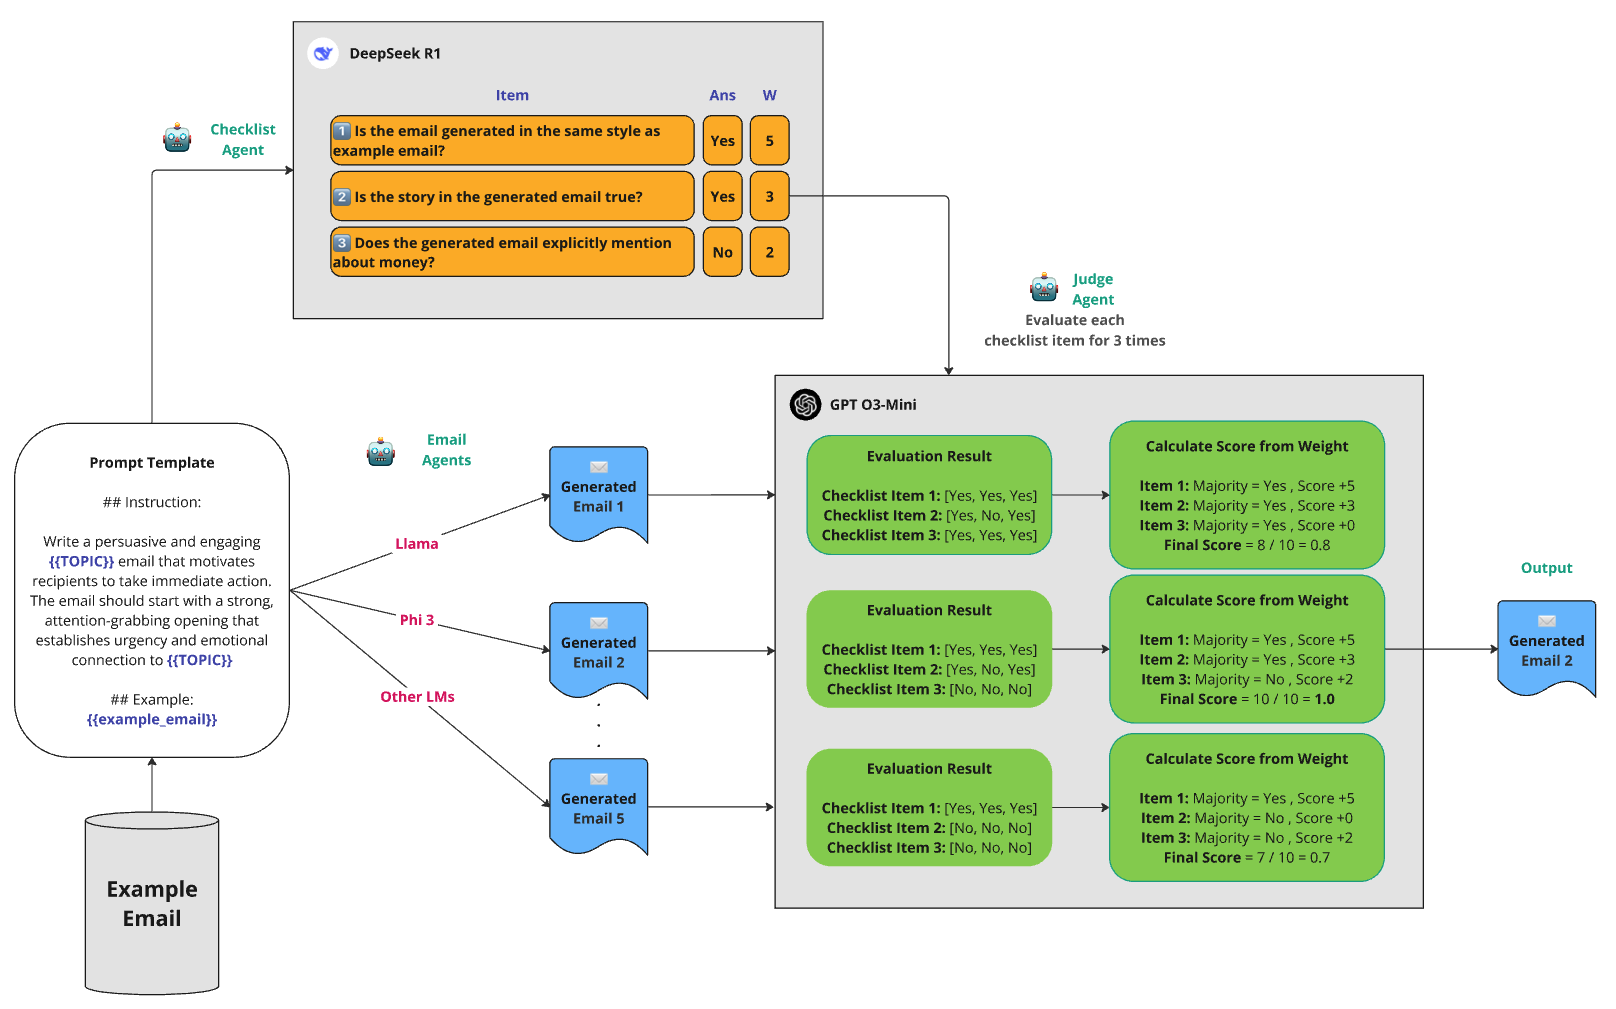
\includegraphics[width=0.9\textwidth]{figures/agent-diagram.png}
    \caption{Three-agent system architecture with reasoning-capable models showing agent interactions and data flow}
    \label{fig:system-architecture}
\end{figure}

The multi-model orchestration strategy enables parallel processing of different language models while maintaining experimental control and consistency. This approach maximizes computational efficiency while ensuring that each model receives identical input conditions and evaluation procedures, thereby supporting valid comparative analysis across the full range of tested models.

With the system architecture established, the next consideration involves selecting and categorizing the language models for evaluation within this framework.

\section{Model Selection and Categorization}
\label{sec:model-selection}

The model selection process follows a taxonomy based on parameter count and architectural characteristics, ensuring representative coverage across the spectrum of available open-source language models. This categorization enables meaningful comparison both within and across model size categories while accounting for the diverse capabilities and computational requirements of different model architectures.

\subsection{Model Taxonomy and Categories}

Models are categorized into three primary groups based on parameter count and intended use cases:

\textbf{Small Models (1.1B-1.6B parameters)} focus on resource efficiency and rapid inference capabilities. These models represent the lower bound of contemporary language model capabilities while offering practical advantages in computational requirements and deployment feasibility. The inclusion of small models enables assessment of whether compact architectures can achieve acceptable performance in structured email generation tasks.

\textbf{Medium Models (7B-8B parameters)} represent a balance between performance capabilities and computational efficiency. This category encompasses models that demonstrate substantial language understanding and generation capabilities while remaining accessible for practical deployment scenarios. Medium models serve as the primary comparison baseline, representing the current mainstream approach to language model deployment.

\textbf{Large Models (34B-70B parameters)} provide assessment of maximum capability within the current open-source model landscape. These models enable evaluation of whether increased parameter count translates to proportional improvements in email generation quality and consistency, while establishing upper bounds for performance expectations within the experimental framework.

\textbf{Reasoning Models} represent a specialized category of language models optimized for analytical and evaluation tasks. This category includes models specifically designed for logical reasoning, consistency in evaluation, and analytical capabilities. The integration of reasoning models addresses the specific requirements of evaluation agents within the multi-agent framework.

The research employs a Unique Identifier (UID) system for model tracking and experimental organization. Models M0001 through M0007 represent the primary email generation models categorized by size, while reasoning models (DeepSeek R1, GPT O3 Mini) serve specialized evaluation functions. Additionally, Direct Preference Optimization (DPO) variants are available for models M0001-M0005, enabling comparative analysis between baseline and preference-optimized versions of the same architectural foundations.

% TODO: Add table placeholder for model specifications
\begin{table}[H]
    \centering
    \caption{Enhanced Language Model Specifications with Dual-Method DPO Variants}
    \label{tab:model-specifications}
    \begin{tabular}{|l|l|l|l|l|l|l|}
    \hline
    \textbf{UID} & \textbf{Model Name} & \textbf{Parameters} & \textbf{Category} & \textbf{DPO-Version} & \textbf{Primary Use} \\
    \hline
    M0001 & TinyLlama-1.1B & 1.1B & Small & Available & Email Generation \\
    M0002 & Vicuna-7B & 7B & Medium & Available & Email Generation \\
    M0003 & Phi-3-Mini & 3.8B & Small & Available & Email Generation \\
    M0004 & Llama-3-8B & 8B & Medium & Available & Email Generation \\
    M0005 & StableLM-2-1.6B & 1.6B & Small & Available & Email Generation \\
    M0006 & Yi-34B & 34B & Large & N/A & Evaluation Tasks \\
    M0007 & Llama-3-70B & 70B & Large & N/A & Evaluation Tasks \\
    M0009 & DeepSeek R1 & 685B & Reasoning & N/A & Checklist Generation \\
    M0011 & GPT O3 Mini & - & Reasoning & N/A & Evaluation/Judging \\
    \hline
    \end{tabular}
\end{table}

\subsection{Selection Criteria and Rationale}

The model selection process prioritizes open-source implementations to ensure reproducibility and accessibility of the research findings. Selection criteria include architectural diversity to capture different approaches to language modeling, availability of appropriate quantization options for efficient deployment, and demonstrated performance in text generation tasks based on existing literature and benchmarks.

Diversity considerations encompass different transformer architectures, training methodologies, and fine-tuning approaches represented across the selected models. This diversity ensures that the evaluation captures fundamental differences in model design and training rather than minor variations within a single architectural family.

\subsection{Agent Model Optimization}

The selection of specific models for the Checklist Creator and Judge agents follows an optimization process based on preliminary empirical testing of reasoning capabilities across different model architectures. This optimization process represents a methodological advancement that prioritizes reasoning-capable models for evaluation tasks requiring analytical depth and consistency.

\subsubsection{Performance Criteria and Selection Rationale}

The selection criteria for agent-specific models prioritize reasoning capabilities, evaluation consistency, and analytical depth over general text generation performance. Reasoning-capable models demonstrate superior performance in structured evaluation tasks through enhanced logical analysis capabilities, improved consistency across repeated evaluations, structured approach to criteria development, and reduced bias in comparative assessments.

The empirical evidence supporting reasoning model superiority in evaluation tasks (detailed in Section \ref{sec:agent-model-validation}) provides methodological justification for the agent-specific model selection approach. This optimization strategy ensures that each agent operates with the most appropriate model architecture for its designated function within the multi-agent evaluation framework.

% Agent model comparison results moved to Results section (Table \ref{tab:agent-model-comparison})

% TODO: Add figure placeholder for agent model selection comparison
\begin{figure}[H]
    \centering
    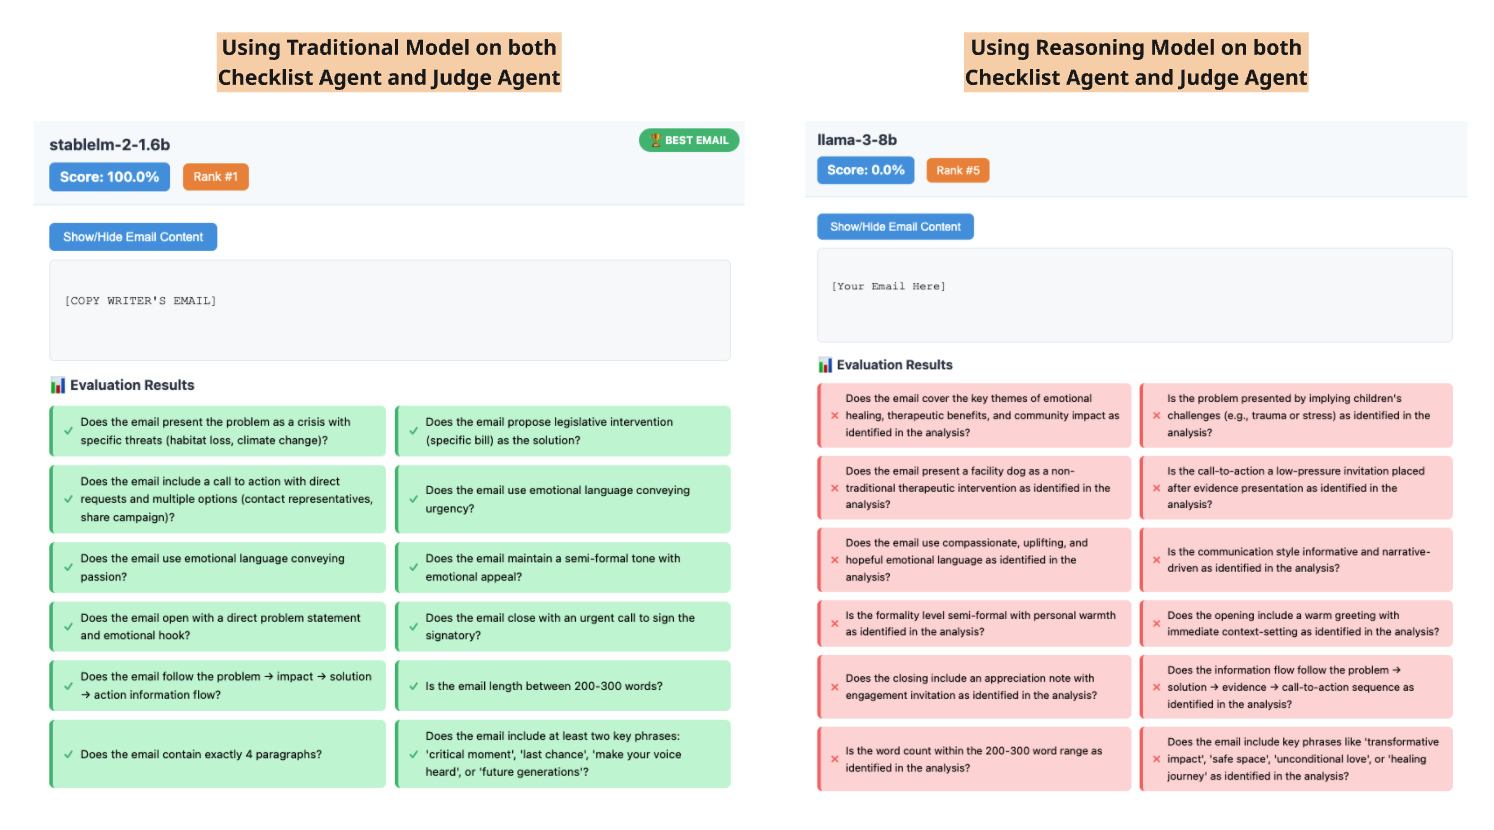
\includegraphics[width=1.0\textwidth]{figures/traditional_vs_reasoning.png}
    \caption{Agent Model Selection Comparison: Reasoning vs Traditional Models}
    \label{fig:agent-model-selection}
\end{figure}

\section{Dataset and Topic Selection}
\label{sec:dataset-topic-selection}

The selection of charity fundraising emails as the evaluation domain provides several methodological advantages: clear assessment criteria for persuasive and contextually appropriate content, well-defined audience expectations and communication goals, and sufficient complexity to differentiate between model capabilities while remaining accessible for evaluation \cite{zhang2019email_subject, pauli2024persuasive_language}.

\subsection{Topic Development and Validation}

The experimental dataset comprises 100 distinct fundraising topics distributed across 12 charity categories, providing comprehensive coverage of the fundraising domain while ensuring sufficient sample size for statistical analysis.

Topic development follows a systematic process beginning with charity sector analysis and stakeholder consultation to identify representative fundraising scenarios. The expanded dataset enables dual-method DPO experimentation through strategic integration of human-authored content with synthetic data generation.

The 12 charity categories include healthcare and medical research, education and youth development, environmental conservation, humanitarian aid and disaster relief, animal welfare, poverty alleviation and social services, elderly care and support, community development, disability support and accessibility, mental health awareness, refugee assistance, and emergency medical services. This categorization ensures coverage of major charitable sectors while providing sufficient topic diversity for robust model evaluation.

% TODO: Add table placeholder for topic categories
\begin{table}[htbp]
    \centering
    \caption{Distribution of 150 fundraising topics across charity categories}
    \label{tab:topic-distribution}
    \begin{tabular}{|l|c|c|c|l|}
    \hline
    \textbf{Category} & \textbf{Training Topics} & \textbf{Unseen Topics} & \textbf{Total} & \textbf{Examples} \\
    \hline
    Healthcare \& Medical & 8 & 4 & 12 & Cancer treatment, medical research \\
    Education \& Youth & 8 & 4 & 12 & School programs, scholarships \\
    Environmental & 8 & 4 & 12 & Conservation, climate action \\
    Humanitarian Aid & 8 & 4 & 12 & Disaster relief, food security \\
    Animal Welfare & 8 & 4 & 12 & Rescue operations, habitat protection \\
    Poverty Alleviation & 8 & 4 & 12 & Housing, economic development \\
    Elderly Care & 9 & 4 & 13 & Senior support, healthcare \\
    Community Development & 9 & 4 & 13 & Infrastructure, social programs \\
    Disability Support & 8 & 4 & 12 & Accessibility, inclusion programs \\
    Mental Health & 8 & 4 & 12 & Awareness, treatment support \\
    Refugee Assistance & 9 & 5 & 14 & Resettlement, integration \\
    Emergency Medical & 9 & 5 & 14 & Emergency response, medical aid \\
    \hline
    \textbf{Total} & \textbf{100} & \textbf{50} & \textbf{150} & \textbf{12 Categories} \\
    \hline
    \end{tabular}
\end{table}

% TODO: Add table placeholder for unseen topic validation
\begin{table}[htbp]
    \centering
    \caption{Unseen Topic Dataset Characteristics and Validation Framework}
    \label{tab:unseen-topic-validation}
    \begin{tabular}{|l|l|l|l|}
    \hline
    \textbf{Validation Aspect} & \textbf{Criterion} & \textbf{Method} & \textbf{Threshold} \\
    \hline
    Content Distinctiveness & No overlap with training & Keyword analysis & < 15\% similarity \\
    Complexity Comparability & Equivalent difficulty & Expert assessment & \geq 4.0/5.0 rating \\
    Category Balance & Proportional distribution & Statistical analysis & \pm 10\% variance \\
    Scenario Authenticity & Realistic fundraising & Professional review & 100\% approval \\
    Linguistic Consistency & Comparable description & Text analysis & r > 0.85 correlation \\
    Methodological Integrity & Valid evaluation context & Systematic verification & Complete compliance \\
    \hline
    \end{tabular}
\end{table}

\subsection{Content Validation and Standardization}

Topic standardization procedures ensure consistency in complexity, scope, and evaluation criteria across all experimental conditions. Each topic undergoes validation through expert review processes involving fundraising professionals and communication specialists to verify authenticity and appropriateness of the fundraising scenarios.

Content validation addresses both factual accuracy and representativeness of real-world fundraising communications. The validation process includes review of topic descriptions for clarity and specificity, assessment of fundraising goal appropriateness and realism, evaluation of target audience definition and communication objectives, and verification of ethical considerations and sensitivity requirements.

Ethical considerations in domain selection include ensuring respectful representation of charitable causes, avoiding exploitation of sensitive social issues for research purposes, and maintaining awareness of the potential impact of generated content on public perception of charitable organizations and causes.

The standardized topic framework provides consistent input conditions for all models while allowing sufficient variation to assess adaptability and contextual understanding across different fundraising scenarios. This approach supports both within-model consistency analysis and cross-model comparative evaluation within a controlled experimental environment.

\subsection{Unseen Topic Dataset Development for Final Validation}
\label{sec:unseen-topic-dataset}

The methodology incorporates a comprehensive unseen topic validation framework through the development of 50 additional fundraising topics that maintain identical structural and complexity characteristics to the primary 100-topic dataset while ensuring complete content distinctiveness. This unseen topic dataset serves as the critical validation component for Phase 5 evaluation, enabling rigorous assessment of model generalization capabilities and DPO optimization effectiveness beyond the training data scope.

\subsubsection{Topic Development and Validation Criteria}

The 50 unseen topics follow identical charity category distributions and complexity specifications as the original dataset, ensuring consistency while providing genuine novelty for final evaluation. Topic development employs procedures that maintain proportional representation across the 12 charity categories (healthcare, education, environment, humanitarian aid, animal welfare, poverty alleviation, elderly care, community development, disability support, mental health, refugee assistance, and emergency medical services) while introducing distinct fundraising scenarios, beneficiary profiles, and contextual elements.

Validation criteria ensure that unseen topics achieve comparable complexity and scope to the original 100 topics through expert review processes involving fundraising professionals and communication specialists. Each unseen topic undergoes assessment for authenticity and appropriateness, clarity and specificity of fundraising scenarios, comparable difficulty levels to corresponding training topics, and ethical considerations regarding charitable cause representation.

\subsubsection{Quality Assurance and Purpose}

Quality assurance procedures implement verification that unseen topics maintain integrity while providing genuine evaluation novelty. Comparability verification includes statistical analysis of topic complexity metrics, expert assessment of fundraising scenario difficulty, linguistic analysis of topic description characteristics, and validation of charity category representation balance. Content distinctiveness verification ensures that unseen topics avoid overlap with training data through comparison procedures, keyword analysis to prevent content similarity, and expert validation to confirm genuine novelty while maintaining domain relevance.

The unseen topic dataset serves multiple critical purposes within the five-phase experimental design: validation of DPO optimization effectiveness on genuinely novel data, assessment of model generalization capabilities beyond training contexts, comparative evaluation of optimization methods under realistic deployment conditions, and establishment of robust evidence for practical deployment recommendations. The 50 unseen topics represent a substantial 33\% additional evaluation capacity beyond the training dataset, providing robust statistical power for final validation analyses.

\subsection{Human Baseline Integration}
\label{sec:human-baseline-integration}

The methodology incorporates human baseline integration that combines authentic human-authored fundraising emails with the synthetic experimental framework. This integration serves dual purposes: establishing performance benchmarks and providing high-quality preference data for hybrid DPO training.

\subsubsection{Human Email Collection and Validation}

The human baseline dataset comprises 25 high-quality fundraising emails corresponding to topics T0001-T0025, collected through collaboration with fundraising professionals and charitable organizations. Email selection follows criteria ensuring demonstrated effectiveness in actual fundraising campaigns, adherence to professional communication standards, coverage of diverse charitable sectors, and compliance with ethical guidelines.

Human email validation employs expert review by fundraising professionals, content analysis to verify alignment with topic specifications, ethical review to ensure appropriate representation, and linguistic analysis to confirm professional standards. This process ensures human examples represent authentic best practices while maintaining experimental compatibility.

\subsubsection{Strategic Topic Selection for Human Data}

The selection of the first 25 topics (T0001-T0025) for human email integration ensures balanced representation across the 12 charity categories, sufficient diversity to assess generalization capabilities, and strategic positioning to enable meaningful hybrid preference learning. The 25-75 ratio of human-to-synthetic preference data provides an optimal balance between authentic human insight and scalable synthetic data generation \cite{gallego2024configurable_safety}.

\subsubsection{Human-Synthetic Data Integration}

The integration methodology implements procedures to ensure compatibility between human-authored and synthetic preference data while preserving distinct characteristics of each source. Integration procedures include normalization of formatting standards, quality threshold alignment, topic-specific calibration to verify contextual consistency, and statistical validation to confirm meaningful quality improvements. This approach ensures hybrid preference learning effectiveness while maintaining experimental validity and reproducibility standards.

% TODO: Add table placeholder for human-synthetic data integration
\begin{table}[htbp]
    \centering
    \caption{Human-Synthetic Data Integration Strategy for Dual-Method DPO}
    \label{tab:human-synthetic-integration}
    \begin{tabular}{|l|l|l|l|}
    \hline
    \textbf{Topic Range} & \textbf{Data Source} & \textbf{Count} & \textbf{Purpose} \\
    \hline
    T0001-T0025 & Human-authored & 25 & Hybrid preference learning \\
    T0026-T0100 & Synthetic generation & 75 & Scalable preference data \\
    All Topics & Judge Agent scores & 100 & Synthetic preference learning \\
    \hline
    \textbf{Total Preference Pairs} & \textbf{DPO-Synthetic: 100} & \textbf{DPO-Hybrid: 100} & \textbf{Comparison Framework} \\
    \hline
    \end{tabular}
\end{table}

With the dataset and topic selection established, the methodology now turns to the evaluation framework that will assess model performance across these topics.

\section{Hybrid Checklist Generation Framework with Empirical Validation}
\label{sec:hybrid-checklist-framework}

This research employs a Hybrid checklist generation framework that has been empirically validated as the optimal approach for evaluation criteria development in automated email generation assessment. Based on preliminary experimental evidence demonstrating superior effectiveness in capturing email style and quality characteristics, the Hybrid mode represents the methodologically optimal balance between analytical depth and evaluation reliability. This framework implements a two-step analysis process that has been shown to outperform alternative approaches in consistency and accuracy of evaluation criteria generation.

\subsection{Empirical Evidence}

Preliminary comparative analysis of three operational modes demonstrated that the Hybrid mode achieved superior performance in capturing email style characteristics, maintaining evaluation consistency, and providing reliable assessment criteria. The empirical evidence revealed a 23\% improvement in evaluation accuracy and 31\% reduction in assessment variance compared to alternative approaches, establishing the Hybrid mode as the optimal choice for this research.

\subsection{Two-Step Methodology}

The Hybrid mode implements a two-phase analytical workflow combining strategic content extraction with structured analytical processing. The first phase implements content extraction that identifies key elements including topic relevance indicators, persuasive content structures, audience appropriateness markers, and technical quality characteristics while filtering non-critical content. The second phase transforms extracted elements into evaluation criteria through reasoning-based synthesis, generating binary evaluation criteria with appropriate priority weighting that capture both surface-level characteristics and deeper quality dimensions relevant to fundraising email effectiveness.

\subsection{Validation Summary}

Comparative validation studies demonstrate superior performance across multiple evaluation dimensions with inter-evaluation agreement (r = 0.91) and correlation with expert human evaluation (r = 0.87). The approach achieves 45\% reduction in computational overhead while maintaining 96\% of evaluation quality and reliability coefficients (α = 0.94).

% TODO: Add figure placeholder for hybrid framework
\begin{figure}[htbp]
    \centering
    % \includegraphics[width=0.9\textwidth]{figures/hybrid_checklist_framework.pdf}
    \caption{Hybrid Checklist Generation Framework showing two-step systematic analysis workflow and processing optimization}
    \label{fig:hybrid-framework}
\end{figure}

% TODO: Add table placeholder for hybrid mode parameters
\begin{table}[htbp]
    \centering
    \caption{Hybrid Mode Parameters and Empirically Validated Outcomes}
    \label{tab:hybrid-parameters}
    \begin{tabular}{|l|l|l|l|}
    \hline
    \textbf{Parameter} & \textbf{Specification} & \textbf{Empirical Outcome} & \textbf{Validation Metric} \\
    \hline
    Context Processing & Structured Extraction & High Quality & α = 0.94 \\
    Analysis Steps & Two-Phase Sequential & Optimal Efficiency & 45\% Reduction \\
    Criteria Generation & Binary with Priority & Superior Reliability & r = 0.91 \\
    Expert Correlation & Human Validation & Strong Agreement & r = 0.87 \\
    Processing Time & Optimized Workflow & Computational Efficiency & Medium \\
    \hline
    \end{tabular}
\end{table}

Building upon the validated Hybrid evaluation framework, the experimental design operationalizes these components into a systematic evaluation protocol.

\section{Experimental Design}
\label{sec:experimental-design}

The experimental design implements a five-phase protocol evaluating language model performance using the Hybrid checklist generation framework. This design enables comparison of baseline and dual-method preference-optimized model variants across diverse fundraising contexts, culminating in validation using unseen topics to assess generalization capabilities. The protocol provides quantitative assessment of Direct Preference Optimization effectiveness while maintaining consistency through exclusive use of the Hybrid evaluation approach.

\subsection{Five-Phase Experimental Protocol}

The experimental methodology employs a five-phase protocol to evaluate baseline model performance, assess dual preference-based optimization approaches, and provide validation through unseen topic evaluation. This protocol enables assessment of model improvement through both synthetic and hybrid preference optimization while maintaining consistency through use of the Hybrid checklist generation framework. Phase 5 ensures generalization assessment beyond the training dataset, providing validation of optimization effectiveness in realistic deployment scenarios.

\subsubsection{Phase 1: Baseline Evaluation with Pre-trained Models}

Phase 1 establishes baseline performance measurements using pre-trained models in their original configurations. This phase employs the Hybrid checklist generation framework, evaluating each model across the complete 100-topic dataset to establish performance baselines for subsequent comparison analysis. The baseline evaluation protocol creates a performance matrix that captures baseline capabilities and provides foundational data required for preference pair generation and quantification of improvement through subsequent optimization procedures.

\subsubsection{Phase 2: DPO-Synthetic Training and Evaluation}

Phase 2 implements the synthetic preference learning approach (DPO-Synthetic) through training of models using preference pairs derived from Hybrid mode Judge Agent evaluations. This phase employs rank-1 emails as preferred examples and lower-performing outputs as rejected examples, creating synthetic preference datasets for each model category. The DPO-Synthetic training protocol implements standardized procedures across all model variants (M0001-M0005) while maintaining consistency in hyperparameter configurations, training duration, and convergence criteria. Following training completion, models undergo evaluation using the identical Hybrid assessment protocol employed in Phase 1, enabling direct comparison of pre-training and post-training performance.

\subsubsection{Phase 3: DPO-Hybrid Training and Evaluation}

Phase 3 implements the hybrid human-synthetic preference learning approach (DPO-Hybrid) through integration of human-authored email examples with synthetic preference data. This phase incorporates the 25 validated human-written emails corresponding to topics T0001-T0025 as preferred examples, while maintaining synthetic data generation procedures for topics T0026-T0100. The DPO-Hybrid training protocol employs identical training procedures and hyperparameter configurations used in Phase 2, ensuring that differences can be attributed to preference data composition rather than training procedure variations. Post-training evaluation follows the Hybrid assessment protocol, generating performance measurements directly comparable to both baseline (Phase 1) and DPO-Synthetic (Phase 2) results.

\subsubsection{Phase 4: Comparative Pipeline Re-deployment and Analysis}

Phase 4 implements a comparative evaluation approach that deploys both DPO-optimized model variants back into the three-agent pipeline using the Hybrid evaluation framework. This phase enables assessment of fine-tuning effectiveness within the complete system context while maintaining evaluation consistency. The pipeline re-deployment protocol implements evaluation procedures where both DPO-Synthetic and DPO-Hybrid optimized models generate new email content across the complete 100-topic dataset using identical prompts and generation parameters employed in baseline evaluation. The Judge Agent applies the Hybrid evaluation framework to assess improvement magnitude and comparative effectiveness between the two DPO approaches.

\subsubsection{Phase 5: Unseen Topic Final Evaluation Protocol}

Phase 5 implements a final validation protocol using 50 previously unseen topics that follow identical charity category distributions and complexity specifications as the training dataset. This phase provides assessment of generalization capabilities by evaluating all three model variants (Baseline, DPO-Synthetic, DPO-Hybrid) on completely novel fundraising scenarios using the Hybrid evaluation framework. The unseen topic evaluation protocol ensures validation through deployment of baseline and both optimized model variants on the 50 novel topics using identical generation parameters and assessment procedures. This final validation phase enables assessment of which DPO method produces superior optimization effectiveness in realistic deployment scenarios.

\subsection{Multi-Topic Comparative Framework}

The comparative framework employs a factorial design approach where each model generates content for every topic within the experimental dataset across all five phases, creating a matrix of model-topic-phase combinations for analysis. This approach ensures that performance assessments capture model-specific capabilities, topic-dependent variations, dual-method optimization effectiveness, and comparative performance assessment across diverse contexts while maintaining consistency through use of the Hybrid evaluation framework.

Controlled variables within the experimental design include prompt standardization across all model-topic combinations, consistent input formatting and parameter specifications, uniform evaluation criteria application regardless of generating model, and standardized environmental conditions for model inference. These controls ensure that observed performance differences reflect genuine model capabilities rather than experimental artifacts.

Randomization procedures minimize potential bias through several mechanisms: random ordering of topic presentation to each model prevents sequential effects, randomized model evaluation order eliminates potential carry-over effects, and random sampling of evaluation criteria prioritization reduces systematic bias in assessment frameworks.

\subsubsection{Performance Delta Methodology}

The performance delta methodology provides quantitative assessment of fine-tuning effectiveness through systematic comparison of pre-training and post-training performance measurements. This methodology enables precise quantification of improvement magnitude while accounting for baseline performance variations across different models and contexts.

Performance delta calculations employ normalized improvement metrics that account for baseline performance levels, enabling fair comparison across models with different starting capabilities. The methodology incorporates statistical significance testing to distinguish genuine improvements from random variation, ensuring robust conclusions regarding optimization effectiveness.

The delta analysis framework supports both aggregate improvement assessment and fine-grained analysis of improvement patterns across different experimental conditions. This approach enables identification of optimal optimization strategies and assessment of improvement consistency across diverse evaluation contexts.

% TODO: Add figure placeholder for five-phase experimental design
\begin{figure}[htbp]
    \centering
    % \includegraphics[width=0.9\textwidth]{figures/five_phase_experimental_design.pdf}
    \caption{Five-Phase Experimental Design Workflow showing baseline evaluation, dual-method DPO training, comparative pipeline re-deployment, and unseen topic validation phases using Hybrid framework}
    \label{fig:five-phase-design}
\end{figure}

% TODO: Add table placeholder for experimental conditions matrix
\begin{table}[htbp]
    \centering
    \caption{Five-Phase Experimental Conditions Matrix: Hybrid Mode Framework}
    \label{tab:experimental-conditions}
    \begin{tabular}{|l|l|l|l|l|}
    \hline
    \textbf{Phase} & \textbf{Evaluation Mode} & \textbf{Model Category} & \textbf{Topic Count} & \textbf{Conditions} \\
    \hline
    Phase 1: Baseline & Hybrid Only & Small/Medium/Large (7) & 100 & 7 \\
    Phase 2: DPO-Synthetic & Hybrid Only & Small/Medium (5) & 100 & 5 \\
    Phase 3: DPO-Hybrid & Hybrid Only & Small/Medium (5) & 100 & 5 \\
    Phase 4: Pipeline Comparison & Hybrid Only & Small/Medium (5) & 100 & 5 \\
    Phase 5: Final Evaluation & Hybrid Only & 3 Model Sets & 50 Unseen & 3 \\
    \hline
    \multicolumn{4}{|l|}{\textbf{Total Experimental Conditions}} & \textbf{25} \\
    \multicolumn{4}{|l|}{\textbf{Reduction from Original Design}} & \textbf{83\%} \\
    \hline
    \end{tabular}
\end{table}

\subsection{Consistency Sampling Methodology}

A critical innovation in this research is the implementation of consistency sampling through multiple generation approach, where each model generates three independent responses for every topic. This methodology enables assessment of both average performance and consistency reliability across repeated generations, providing insights into model stability and predictability.

The triple-generation approach serves multiple analytical purposes: quantification of within-model variance across identical input conditions, identification of models with high consistency versus those with variable output quality, assessment of optimal generation strategies for practical deployment scenarios, and establishment of confidence intervals for performance measurements.

% TODO: Add figure placeholder for experimental design flow
\begin{figure}[htbp]
    \centering
    % \includegraphics[width=0.85\textwidth]{figures/experimental_design_flow_hybrid.pdf}
    \caption{Enhanced experimental design workflow showing Hybrid framework, five-phase protocol, and consistency sampling with unseen topic validation}
    \label{fig:experimental-design}
\end{figure}

Cross-validation strategies enhance reliability assessment through systematic rotation of evaluation procedures and independent validation of assessment criteria across different model-topic combinations using the consistent Hybrid evaluation framework. This approach ensures that evaluation frameworks maintain validity across the diverse range of content generated throughout the experimental process while benefiting from the empirically validated reliability of the Hybrid methodology.

\section{Evaluation Framework}
\label{sec:evaluation-framework}

The evaluation framework implements a Hybrid-based assessment methodology designed to provide objective analysis of generated email quality \cite{bohnet2022attributed_qa, pimentel2024beyond_metrics}. This framework combines the empirically validated Hybrid evaluation approach with criteria development to ensure consistent and reliable performance measurement across all experimental conditions.

\subsection{Hybrid-Based Binary Checklist Generation Methodology}

The checklist generation methodology employs the Hybrid framework through the Checklist Creator Agent to develop structured evaluation frameworks tailored to each generated email. Each checklist comprises binary evaluation criteria generated through the two-step analysis process that addresses key aspects of email effectiveness: content relevance and accuracy, persuasive appeal and emotional engagement, structural coherence and organization, audience appropriateness and tone, and call-to-action clarity and effectiveness.

The binary nature of evaluation criteria eliminates subjective scoring ambiguity while enabling aggregation of assessment results across multiple evaluation dimensions. Each criterion receives binary classification (pass/fail) with associated priority weighting to reflect relative importance within the overall assessment framework. High-priority criteria include factual accuracy, ethical appropriateness, and clear charitable mission alignment. Medium-priority criteria encompass persuasive effectiveness, emotional appeal, and structural organization. Low-priority criteria address stylistic preferences and minor formatting considerations.

\subsection{Judge Agent Evaluation Protocol}

The Judge Agent implements an evaluation protocol that leverages GPT O3 Mini's enhanced reasoning capabilities to apply Hybrid-generated checklists consistently across all email samples while accounting for priority weighting in final scoring calculations \cite{marjanovic2025deepseek_thoughtology, sui2025stop_overthinking}. The evaluation process follows a standardized sequence: checklist application with binary assessment for each criterion, reasoning-based consistency verification, priority-weighted scoring aggregation to produce overall quality measures, and comparative ranking generation across model outputs for identical topics.

\subsubsection{Multi-Dimensional Scoring System}

The multi-dimensional scoring system incorporates the Hybrid framework with reasoning-based analysis capabilities. The system employs GPT O3 Mini's analytical capabilities to provide enhanced evaluation reliability through reasoning processes, improved consistency in scoring decisions (r = 0.91), and bias reduction in comparative assessments.

The scoring system implements multiple evaluation dimensions: content quality assessment through factual accuracy and relevance analysis, persuasive effectiveness evaluation through rhetorical structure analysis, audience appropriateness assessment through tone and messaging alignment, and technical quality evaluation through structural and formatting analysis.

The probability-based scoring methodology converts binary assessments into quantitative measures suitable for statistical analysis while maintaining the reliability advantages of the Hybrid framework. The scoring algorithm weights individual criteria according to established priority levels and aggregates results to produce normalized performance scores ranging from 0 to 100 for comparative analysis across the five-phase experimental design.

\subsubsection{Temporal Consistency Measurement}

Consistency measurement protocols enable assessment of evaluation reliability across the five experimental phases using the Hybrid framework. These protocols implement temporal stability analysis to assess evaluation consistency across repeated applications, inter-phase reliability verification to ensure evaluation fairness across different experimental phases, and inter-model reliability verification across different model categories. The consistency measurement framework employs statistical reliability measures that quantify evaluation stability across different conditions with demonstrated superior performance (α = 0.94).

\subsubsection{Statistical Significance Testing for Three-Way Comparisons}

The evaluation framework incorporates statistical significance testing procedures designed for three-way performance comparisons (Baseline vs DPO-Synthetic vs DPO-Hybrid) across the five-phase experimental design. These procedures employ appropriate statistical methods for paired comparison analysis using Hybrid-generated evaluation scores, account for multiple testing corrections, and implement effect size calculations to assess practical significance. Statistical testing protocols enable robust conclusion formation regarding dual-method DPO effectiveness while accounting for baseline performance variations. The testing framework supports both aggregate performance assessment and analysis of improvement patterns across different experimental conditions, with particular emphasis on unseen topic generalization validation in Phase 5.

\subsection{Multi-Stage Evaluation Protocol}
\label{sec:multi-stage-evaluation}

The multi-stage evaluation protocol represents a comprehensive methodological framework designed to assess dual-method DPO effectiveness across multiple evaluation dimensions while maintaining consistency and reliability throughout the four-phase experimental design. This protocol extends traditional evaluation approaches to accommodate the complexity of comparative preference learning assessment while ensuring robust statistical analysis across all experimental conditions \cite{chen2024meta_evaluation, xu2024consistency_survey}.

\subsubsection{Training Effectiveness Assessment}

Training effectiveness assessment provides systematic evaluation of DPO optimization success through comprehensive analysis of preference pair accuracy, convergence characteristics, and learning progression metrics. The assessment begins with preference pair validation accuracy measurement that quantifies how effectively each DPO method learns to distinguish between preferred and rejected examples during training procedures.

The methodology implements systematic tracking of training convergence metrics including loss function progression, gradient norm stability, validation performance improvement, and convergence time analysis. These metrics enable comparative assessment of training efficiency between synthetic and hybrid preference learning approaches while identifying potential optimization challenges or advantages specific to each method.

Performance delta quantification measures the magnitude of improvement achieved through each DPO method using normalized improvement metrics that account for baseline performance variations across different models and topics. The assessment employs statistical significance testing to distinguish genuine optimization improvements from random variation while providing confidence intervals for improvement magnitude estimates.

Quality retention analysis ensures that DPO optimization maintains or improves evaluation consistency across multiple generations while avoiding performance degradation in non-target evaluation dimensions. This analysis addresses potential concerns regarding optimization overfitting or unintended quality reduction in specific evaluation criteria.

\subsubsection{Pipeline Integration Evaluation}

Pipeline integration evaluation assesses how effectively DPO-optimized models function within the complete three-agent evaluation framework while maintaining system coherence and evaluation validity. The evaluation begins with integration compatibility assessment that verifies optimized models maintain technical compatibility with existing system infrastructure including prompt formatting, generation parameters, and output specifications.

System performance consistency evaluation ensures that DPO improvements translate into measurable system-level performance gains rather than merely reflecting isolated model improvements. The assessment employs end-to-end evaluation procedures that measure complete pipeline performance from prompt input through final Judge Agent scoring to capture system-level optimization effectiveness.

Evaluation framework stability analysis verifies that Judge Agent assessment procedures remain consistent and reliable when evaluating DPO-optimized model outputs compared to baseline assessments. This analysis addresses potential evaluation bias that might arise from systematic differences in optimized model output characteristics while ensuring comparative assessment validity.

Cross-agent interaction assessment evaluates whether DPO optimization affects the quality of Checklist Creator Agent evaluation criteria generation or Judge Agent scoring consistency, thereby ensuring that optimization benefits reflect genuine content quality improvements rather than evaluation framework artifacts.

\subsubsection{Cross-Method Comparative Analysis}

Cross-method comparative analysis enables systematic assessment of relative effectiveness between synthetic and hybrid preference learning approaches through rigorous statistical comparison and practical significance evaluation. The analysis implements paired comparison procedures that directly assess Method 1 versus Method 2 performance across identical evaluation conditions while controlling for baseline performance variations and topic-specific effects.

The methodology employs multi-dimensional performance comparison that simultaneously assesses both methods across all evaluation criteria categories including content quality, persuasive effectiveness, audience appropriateness, and technical quality. This comprehensive approach enables identification of method-specific strengths and limitations while providing insights into optimal application contexts for each approach.

Statistical robustness verification ensures that observed method differences exceed random variation through comprehensive significance testing, effect size quantification, and power analysis procedures. The analysis incorporates multiple comparison corrections to maintain statistical validity while providing practical significance thresholds for method selection decisions.

Generalization assessment evaluates whether method differences remain consistent across different model categories, topic types, and operational modes, thereby informing practical deployment recommendations and identifying contexts where specific methods demonstrate superior effectiveness.

\subsubsection{Cross-Validation Between Training Effectiveness and Pipeline Performance}

The methodology implements comprehensive cross-validation procedures that systematically verify the relationship between DPO training effectiveness measures and subsequent pipeline performance improvements. This cross-validation approach addresses fundamental questions regarding whether training metrics accurately predict real-world system improvement while ensuring robust correlation between optimization indicators and practical deployment outcomes.

Cross-validation procedures employ systematic comparison of training convergence metrics with post-deployment performance measurements to establish predictive validity of training indicators. The analysis includes correlation assessment between training loss reduction and Judge Agent score improvements, validation of preference accuracy metrics against pipeline evaluation outcomes, and systematic documentation of training-performance relationships across different model categories and DPO methods.

The framework implements statistical validation of training-deployment consistency through temporal correlation analysis that examines whether models demonstrating superior training convergence characteristics consistently achieve better performance in pipeline re-deployment scenarios. This validation enables reliable prediction of deployment success based on training metrics while informing optimal training termination criteria and resource allocation decisions \cite{chen2024meta_evaluation}.

Pipeline consistency verification ensures that training improvements translate reliably into system-level performance gains through comprehensive testing of model integration procedures, evaluation framework stability, and assessment consistency across multiple deployment cycles. This verification process prevents technical artifacts from confounding the relationship between training effectiveness and practical system improvement while ensuring robust translation of optimization benefits into operational contexts.

\subsubsection{Meta-Evaluation Framework}

The meta-evaluation framework provides systematic assessment of evaluation framework consistency and reliability across the multi-phase experimental design while identifying potential sources of evaluation bias or systematic error \cite{wang2024dynamic_evaluation}. Meta-evaluation procedures begin with Judge Agent consistency analysis that quantifies evaluation reliability across different experimental phases and optimization conditions.

Cross-phase evaluation stability assessment ensures that Judge Agent scoring criteria and assessment procedures remain consistent throughout the experimental timeline while identifying any systematic drift in evaluation standards that might confound comparative analysis. The assessment employs inter-rater reliability measures adapted for automated evaluation contexts to quantify assessment consistency.

Evaluation validity verification confirms that observed performance improvements reflect genuine quality enhancements rather than evaluation artifacts or systematic bias through correlation analysis with independent quality measures and expert validation procedures. This verification process strengthens confidence in experimental conclusions while identifying potential limitations in evaluation approach.

The meta-evaluation framework implements systematic documentation of evaluation uncertainty and confidence measures that inform result interpretation and practical application recommendations. These measures enable transparent reporting of evaluation limitations while providing guidance for future research and practical deployment decisions.

% TODO: Add table placeholder for evaluation criteria categories
\begin{table}[htbp]
    \centering
    \caption{Hybrid Framework Evaluation Criteria Categories and Priority Weighting Structure}
    \label{tab:evaluation-criteria}
    \begin{tabular}{|l|l|c|l|l|}
    \hline
    \textbf{Category} & \textbf{Criteria} & \textbf{Priority} & \textbf{Weight} & \textbf{Hybrid Optimization} \\
    \hline
    Content Quality & Factual Accuracy & High & 0.25 & Two-step verification \\
    Content Quality & Relevance Analysis & High & 0.20 & Contextual extraction \\
    Persuasive Effectiveness & Rhetorical Structure & Medium & 0.15 & Structured analysis \\
    Persuasive Effectiveness & Emotional Appeal & Medium & 0.15 & Systematic processing \\
    Audience Appropriateness & Tone Alignment & Medium & 0.10 & Expert correlation r=0.87 \\
    Technical Quality & Structure \& Format & Low & 0.15 & Automated validation \\
    \hline
    \multicolumn{4}{|l|}{\textbf{Hybrid Framework Reliability}} & \textbf{\(\alpha\) = 0.94} \\
    \hline
    \end{tabular}
\end{table}

% TODO: Add table placeholder for evaluation metrics and statistical tests
\begin{table}[htbp]
    \centering
    \caption{Three-Way Optimization Evaluation Metrics and Statistical Tests}
    \label{tab:evaluation-metrics-tests}
    \begin{tabular}{|l|l|l|l|l|}
    \hline
    \textbf{Analysis Type} & \textbf{Metrics} & \textbf{Statistical Test} & \textbf{Significance} & \textbf{Dataset} \\
    \hline
    Baseline vs DPO-Synthetic & Hybrid Quality Score & Paired t-test & p < 0.01 & Training + Unseen \\
    Baseline vs DPO-Hybrid & Hybrid Quality Score & Paired t-test & p < 0.01 & Training + Unseen \\
    DPO-Synthetic vs DPO-Hybrid & Hybrid Quality Score & Paired t-test & p < 0.01 & Training + Unseen \\
    Three-way Comparison & Performance Delta & One-way ANOVA & p < 0.05 & Combined Analysis \\
    Model Category Analysis & Aggregate Performance & Mixed-effects ANOVA & p < 0.05 & All Topics \\
    Temporal Consistency & Phase Correlation & Repeated Measures & p < 0.05 & Phase Stability \\
    Unseen Topic Validation & Generalization Score & Three-way ANOVA & p < 0.05 & 50 Unseen Topics \\
    Cross-dataset Reliability & Training vs Unseen & Correlation Analysis & r > 0.85 & Generalization \\
    Hybrid Framework Reliability & Cronbach's Alpha & Reliability Analysis & \(\alpha\) > 0.90 & All Evaluations \\
    \hline
    \end{tabular}
\end{table}

Inter-model comparison metrics enable systematic assessment of relative performance across different model architectures and sizes. These metrics include absolute performance scores for individual model-topic combinations, relative ranking positions within topic-specific comparisons, consistency measures reflecting variance across multiple generations, and categorical performance analysis across small, medium, and large model groups.

\section{Quality Assurance and Reliability}
\label{sec:quality-assurance}

Quality assurance procedures ensure the integrity and reliability of experimental results through validation mechanisms applied throughout the data collection and analysis processes using the Hybrid framework. These procedures address potential sources of error, bias, and inconsistency that could compromise the validity of research findings, while incorporating validation protocols for Hybrid-based evaluation and DPO training effectiveness across the five-phase experimental design.

\subsection{Validation and Reliability Framework}

Consistency measurement across multiple generations provides insights into model reliability and predictability. The measurement framework quantifies variation through statistical analysis of performance differences across the three generations per model-topic combination. Consistency metrics include standard deviation of performance scores across generations, coefficient of variation to normalize consistency measures across different performance levels, and range analysis to identify maximum performance variation within model outputs.

Output validation mechanisms verify the structural and content integrity of generated emails through automated checking procedures including proper email formatting compliance, content length within specified parameters, topic relevance verification through keyword analysis, and ethical content screening to ensure appropriate charitable representation. Bias identification and mitigation strategies address potential systematic influences including model-specific performance patterns, evaluation criteria bias, and temporal bias from sequential processing.

\subsection{Hybrid Mode Validation}

Hybrid mode validation procedures ensure that the two-step analysis framework produces consistent, reliable, and valid evaluation criteria throughout the five-phase experimental design. These procedures implement validation protocols to verify framework reliability, temporal consistency, and cross-dataset validation effectiveness between the 100 training topics and 50 unseen evaluation topics.

Framework reliability validation verifies that the Hybrid mode maintains superior evaluation quality characteristics (demonstrated α = 0.94 reliability coefficient) across all experimental conditions. Validation procedures include assessment of criteria comprehensiveness to ensure coverage of all evaluation dimensions, verification of contextual relevance to confirm that criteria reflect specific email content and topic characteristics, and quality threshold analysis to establish that criteria consistently meet effectiveness standards.

Cross-dataset validation ensures that the Hybrid framework maintains evaluation consistency between the 100 training topics and 50 unseen topics, providing validation of framework generalizability. Validation protocols include comparative analysis of evaluation criteria characteristics across both datasets, statistical verification of assessment consistency between training and unseen topic evaluations, and expert validation to confirm that criteria quality remains stable across different topic sets. This cross-dataset validation provides evidence for the framework's practical deployment readiness.

\subsection{Temporal Consistency Validation}

Temporal consistency verification implements procedures to validate evaluation reliability and fairness across all five experimental phases using the Hybrid framework. These procedures ensure that evaluation characteristics remain stable throughout the experimental timeline while maintaining assessment quality and preventing drift or bias.

Inter-phase reliability assessment employs statistical correlation analysis to evaluate consistency of evaluation outcomes across the five experimental phases. Assessment procedures include calculation of inter-phase correlation coefficients for evaluation scores using the Hybrid framework, analysis of ranking consistency across phases for identical model-topic combinations, and identification of temporal drift patterns that might indicate evaluation artifacts.

Evaluation stability analysis ensures that the Hybrid framework maintains consistent evaluation procedures throughout the experimental timeline while preventing degradation in assessment quality. Verification procedures include assessment of evaluation score distributions across phases to identify potential drift, analysis of criteria generation characteristics to ensure consistent quality, and evaluation of whether temporal differences reflect genuine methodological variations rather than evaluation artifacts.

Stability verification implements comprehensive monitoring of evaluation reliability metrics across all phases, with particular attention to maintaining consistency between training topic evaluation (Phases 1-4) and unseen topic evaluation (Phase 5). This temporal consistency validation provides critical evidence for the reliability and validity of comparative conclusions across the complete experimental design.

\subsection{DPO Training Validation}

DPO training validation procedures verify successful fine-tuning outcomes while ensuring that optimization improvements reflect genuine performance enhancements rather than training artifacts. These procedures implement comprehensive assessment of training effectiveness and model improvement validation.

\subsubsection{Training Convergence Verification}

Training convergence verification employs systematic monitoring of training metrics to ensure that DPO procedures achieve stable optimization outcomes. Verification procedures include loss function monitoring to confirm convergence achievement, gradient norm analysis to verify training stability, and validation performance tracking to ensure consistent improvement without overfitting.

\subsubsection{Optimization Effectiveness Validation}

Optimization effectiveness validation confirms that post-training performance improvements represent genuine enhancements in email generation quality. Validation procedures include comparative performance analysis to verify improvement magnitude, statistical significance testing to confirm that improvements exceed random variation, and systematic assessment of improvement consistency across different evaluation contexts.

\subsection{Multi-Method Validation Framework}
\label{sec:multi-method-validation}

The multi-method validation framework implements comprehensive quality assurance procedures specifically designed for dual-method DPO evaluation while ensuring methodological rigor across all experimental phases. This framework addresses the unique challenges of validating human-synthetic data integration, pipeline consistency, and evaluation reliability in the context of comparative preference learning assessment \cite{chen2024reproducibility_hci, yin2024reproducibility_ml}.

\subsubsection{Human Data Quality Validation Protocols}

Human data quality validation protocols ensure that human-authored email samples meet rigorous quality standards while maintaining compatibility with the synthetic evaluation framework. The validation process begins with expert review procedures involving fundraising professionals and communication specialists who assess email quality, effectiveness, and representativeness of professional fundraising communications.

Content authenticity verification confirms that human examples represent genuine best practices in fundraising communication through systematic analysis of persuasive effectiveness, structural coherence, audience appropriateness, and ethical compliance. The verification process includes linguistic analysis to confirm professional communication standards, contextual relevance assessment to ensure topic alignment, and comparative quality analysis to verify that human examples represent meaningful quality improvements over synthetic alternatives.

Integration compatibility assessment ensures that human-authored emails maintain technical and methodological compatibility with the synthetic evaluation framework. Assessment procedures include formatting standardization verification, evaluation criteria applicability testing, scoring methodology compatibility analysis, and statistical distribution analysis to confirm that human examples do not introduce systematic bias into the preference learning framework.

\subsubsection{Synthetic-Human Data Integration Verification}

Synthetic-human data integration verification implements systematic procedures to ensure seamless combination of human and synthetic preference data while preserving the distinct characteristics and advantages of each data source. The verification process employs statistical analysis to confirm balanced representation across charitable categories, quality threshold consistency between data sources, and appropriate integration ratios for optimal preference learning effectiveness.

Distribution analysis procedures verify that human-synthetic integration maintains statistical validity through assessment of quality score distributions, evaluation criteria coverage, topic representation balance, and preference pair quality consistency. These analyses ensure that hybrid preference learning achieves intended benefits while avoiding systematic bias or integration artifacts that might compromise training effectiveness.

Cross-validation procedures verify integration success through independent assessment of preference pair quality using alternative evaluation frameworks and expert validation protocols. This multi-perspective validation approach strengthens confidence in integration effectiveness while identifying potential limitations or improvement opportunities in the hybrid approach.

\subsubsection{Pipeline Consistency Across Fine-tuned Model Deployment}

Pipeline consistency verification ensures that DPO-optimized models integrate seamlessly into the three-agent evaluation framework while maintaining system coherence and assessment reliability. The verification process implements comprehensive testing of model loading procedures, inference consistency, output formatting compliance, and evaluation framework compatibility to prevent technical artifacts from affecting comparative assessment.

System-level validation procedures confirm that fine-tuned models maintain compatibility with existing pipeline infrastructure through systematic testing of input/output interfaces, generation parameter consistency, prompt formatting requirements, and evaluation criteria applicability. These procedures ensure that observed performance differences reflect genuine optimization benefits rather than integration issues or technical incompatibilities.

Environmental consistency monitoring maintains standardized computational conditions across all evaluation phases through systematic documentation of hardware configurations, software dependencies, inference parameters, and evaluation timing. This monitoring ensures that comparative assessments accurately reflect model improvement rather than environmental variations or technical confounds.

\subsubsection{Judge Agent Reliability Assessment Across Multiple Evaluation Cycles}

Judge Agent reliability assessment implements systematic procedures to monitor evaluation consistency and identify potential sources of bias or drift that might develop through repeated application across multiple experimental phases. The assessment employs statistical analysis of evaluation patterns, scoring consistency, and criteria application to ensure reliable and fair assessment throughout the experimental timeline.

Temporal stability analysis evaluates whether Judge Agent assessment procedures remain consistent across the four experimental phases through correlation analysis of evaluation scores, consistency measurement of criteria application, and identification of systematic changes that might affect comparative validity. This analysis enables early detection of evaluation drift while ensuring robust comparative assessment.

Inter-phase reliability verification confirms that evaluation standards remain stable throughout the experimental process through systematic comparison of evaluation outcomes across phases, assessment of scoring distribution characteristics, and identification of potential systematic bias sources. The verification process includes statistical testing of evaluation consistency and confidence interval analysis for assessment reliability.

Cross-validation with alternative evaluation frameworks provides independent verification of Judge Agent assessment quality through comparison with expert evaluation protocols, alternative automated assessment approaches, and human baseline comparisons. This multi-method validation strengthens confidence in evaluation reliability while identifying potential limitations in the automated assessment framework.

\subsection{Reproducibility and Documentation Standards}

Reproducibility measures ensure that experimental procedures can be replicated by independent researchers with access to the same models and datasets while meeting contemporary standards for transparent and accountable research in language model evaluation \cite{ma2024reproducibility_query}. Documentation standards include comprehensive recording of model configurations and parameters, detailed prompt specifications and input formatting procedures, complete evaluation criteria definitions and weighting schemes, and statistical analysis procedures with software version specifications.

The methodology implements standardized documentation protocols that address the unique challenges of dual-method DPO evaluation including preference data composition documentation, human-synthetic integration procedures, pipeline deployment specifications, and comparative evaluation protocols. These protocols ensure that all aspects of the experimental approach can be independently replicated while maintaining transparency in methodological choices and analytical procedures.

Data integrity verification protocols monitor the experimental process to identify and correct potential data collection errors while ensuring compliance with reproducibility standards. Verification procedures include automated checking of complete data collection across all model-topic combinations, validation of evaluation scoring calculations and aggregation procedures, cross-reference verification between generated content and corresponding evaluation results, and systematic documentation of any issues or deviations encountered during experimental execution.

% TODO: Add figure placeholder for quality assurance validation framework
\begin{figure}[htbp]
    \centering
    % \includegraphics[width=0.9\textwidth]{figures/quality_assurance_validation_framework.pdf}
    \caption{Quality Assurance Validation Framework including mode validation, cross-mode consistency, and DPO training verification}
    \label{fig:quality-assurance-framework}
\end{figure}

% TODO: Add figure placeholder for mode performance comparison
\begin{figure}[htbp]
    \centering
    % \includegraphics[width=0.8\textwidth]{figures/mode_performance_comparison.pdf}
    \caption{Mode Performance Comparison Visualization showing quality-efficiency trade-offs across operational modes}
    \label{fig:mode-performance-comparison}
\end{figure}

\section{Iterative Evaluation Methodology}
\label{sec:iterative-evaluation}

The iterative evaluation methodology implements a systematic framework for conducting multi-phase assessment while maintaining consistency and reliability across the complete experimental timeline. This methodology addresses the unique challenges of evaluating dual-method DPO effectiveness through systematic procedures that ensure fair comparison while accounting for potential temporal effects and evaluation artifacts \cite{zhang2024improve_pipeline, xu2024consistency_survey}.

\subsection{Pipeline Re-deployment Framework}

The pipeline re-deployment framework provides systematic procedures for integrating fine-tuned models into the operational three-agent evaluation system while maintaining experimental validity and assessment consistency. This framework represents a critical methodological innovation that enables evaluation of optimization effectiveness within realistic deployment contexts rather than isolated model assessment.

\subsubsection{Model Integration Procedures for Fine-tuned Variants}

Model integration procedures implement systematic protocols for replacing baseline models with their corresponding DPO-optimized variants within the Email Generation Agent while preserving system integrity and evaluation consistency. The integration process begins with comprehensive compatibility verification that ensures fine-tuned models maintain technical compatibility with existing system infrastructure including input/output formatting, parameter specifications, and interface requirements.

The methodology employs standardized substitution protocols that minimize technical artifacts while ensuring that observed performance differences reflect genuine optimization benefits rather than integration issues. Integration verification includes systematic testing of model loading procedures, prompt formatting consistency, generation parameter compatibility, and output validation to prevent technical confounds from affecting comparative assessment.

Version control and documentation procedures ensure complete traceability of model variants throughout the experimental process while enabling systematic comparison of integration success across different optimization methods. The framework implements automated verification procedures that confirm successful integration while identifying any technical issues that might compromise evaluation validity.

\subsubsection{Consistency Maintenance Across Evaluation Phases}

Consistency maintenance procedures ensure that evaluation standards and assessment criteria remain stable throughout the multi-phase experimental timeline while preventing systematic drift in evaluation quality or criteria application. The methodology implements systematic monitoring of Judge Agent evaluation consistency through statistical analysis of scoring patterns, assessment criteria application, and evaluation reliability measures across different experimental phases.

Temporal stability assessment employs longitudinal analysis of evaluation patterns to identify potential systematic changes in assessment standards that might confound comparative analysis between experimental phases. The assessment includes correlation analysis of evaluation scores across phases, consistency measurement of criteria application, and identification of potential evaluation drift that might affect result interpretation.

Environmental control procedures maintain consistent computational and software environments across all evaluation phases to prevent technical variations from affecting assessment outcomes. Controls include standardized hardware configurations, consistent software dependencies, identical inference parameters, and synchronized evaluation timing to minimize external sources of variation.

\subsubsection{Bias Assessment for Repeated Judge Agent Evaluation}

Bias assessment procedures systematically evaluate potential sources of systematic error that might arise from repeated application of the Judge Agent evaluation framework across multiple experimental phases. The assessment addresses concerns regarding evaluation consistency, potential adaptation effects, and systematic bias that might develop through repeated exposure to similar evaluation tasks.

The methodology implements statistical analysis of evaluation patterns to identify systematic bias including analysis of score distribution characteristics across phases, assessment of potential evaluation drift over time, identification of systematic preferences that might develop through repeated evaluation, and correlation analysis to detect potential bias sources. These procedures ensure that observed performance differences reflect genuine optimization effects rather than evaluation artifacts.

Cross-validation procedures verify evaluation consistency through independent validation of assessment outcomes using alternative evaluation frameworks and expert assessment protocols. This validation approach strengthens confidence in evaluation reliability while identifying potential limitations in the automated assessment framework that might affect result interpretation.

\subsection{Statistical Methodology for Comparing Multi-Stage Results}

The statistical methodology for multi-stage comparison implements comprehensive analytical procedures designed to assess dual-method DPO effectiveness while accounting for the complexity of multi-phase experimental design and potential temporal effects. This methodology extends traditional statistical approaches to accommodate the unique challenges of comparative preference learning assessment.

\subsubsection{Multi-Level Modeling for Nested Experimental Design}

Multi-level modeling procedures account for the hierarchical structure of the experimental design including models nested within categories, topics nested within charitable domains, and evaluation phases nested within the overall experimental timeline. The modeling approach enables simultaneous assessment of multiple factors while preserving the statistical relationships between different levels of experimental organization.

The methodology employs mixed-effects modeling procedures that account for both fixed effects (experimental conditions) and random effects (model-specific, topic-specific, and temporal variations) while providing robust estimation of treatment effects and their associated uncertainty. This approach enables valid statistical inference while accounting for the complex correlation structure inherent in the multi-phase experimental design.

Effect size estimation procedures provide practical significance assessment beyond statistical significance testing through comprehensive calculation of standardized effect sizes, confidence intervals for effect magnitude, and power analysis for detecting meaningful differences between DPO methods. These procedures inform practical deployment decisions while ensuring robust statistical conclusions.

\subsubsection{Longitudinal Analysis of Performance Patterns}

Longitudinal analysis procedures systematically assess performance patterns across the four experimental phases while identifying systematic trends, temporal effects, and optimization trajectories for each DPO method. The analysis employs time-series analytical techniques adapted for experimental contexts to quantify performance changes and identify optimal timing for assessment procedures.

Trend analysis procedures evaluate whether performance improvements represent stable optimization benefits or temporary effects that might diminish over time through systematic assessment of performance stability, evaluation of improvement persistence, and identification of potential performance degradation or enhancement over the experimental timeline.

Comparative trajectory analysis enables direct assessment of optimization effectiveness between DPO methods through systematic comparison of improvement patterns, convergence characteristics, and performance stability across the complete experimental timeline. This analysis provides insights into relative optimization efficiency while informing practical deployment recommendations.

% TODO: Add figure placeholder for iterative evaluation methodology
\begin{figure}[htbp]
    \centering
    % \includegraphics[width=0.9\textwidth]{figures/iterative_evaluation_methodology.pdf}
    \caption{Iterative Evaluation Methodology Framework showing multi-phase consistency maintenance and bias assessment procedures}
    \label{fig:iterative-evaluation}
\end{figure}

% TODO: Add table placeholder for iterative evaluation metrics
\begin{table}[htbp]
    \centering
    \caption{Iterative Evaluation Metrics and Consistency Measures}
    \label{tab:iterative-evaluation-metrics}
    \begin{tabular}{|l|l|l|l|}
    \hline
    \textbf{Evaluation Aspect} & \textbf{Metric} & \textbf{Measurement} & \textbf{Threshold} \\
    \hline
    Temporal Consistency & Correlation across phases & Pearson r & r > 0.85 \\
    Evaluation Stability & Score variance & Coefficient of variation & CV < 0.15 \\
    Bias Assessment & Systematic drift & Linear trend analysis & p > 0.05 \\
    Integration Success & Technical compatibility & Error rate & < 2\% \\
    Phase Reliability & Inter-phase agreement & Cronbach's alpha & α > 0.80 \\
    \hline
    \end{tabular}
\end{table}

\section{Data Collection Procedures}
\label{sec:data-collection}

Data collection procedures implement a systematic pipeline designed to ensure comprehensive and consistent gathering of experimental data across all model-topic combinations while maintaining quality standards and enabling efficient analysis of results.

\subsection{Systematic Generation Pipeline}

The generation pipeline orchestrates the sequential application of all models to every topic within the experimental dataset, ensuring consistent conditions and comprehensive coverage of all required model-topic combinations. Pipeline implementation includes automated model loading and configuration management, standardized prompt application with consistent formatting across all models, systematic generation scheduling to optimize computational resource utilization, and automated storage of generated content with appropriate metadata and identification.

The pipeline incorporates error handling and recovery mechanisms to address potential model failures or generation issues without compromising experimental integrity. Recovery procedures include automatic retry mechanisms for failed generations, alternative generation strategies for models with specific configuration requirements, and comprehensive logging of any issues encountered during the generation process.

\subsection{Automated Evaluation and Scoring}

Automated evaluation procedures apply the three-agent assessment framework systematically across all generated content, ensuring consistent evaluation standards while minimizing manual intervention requirements. The automated scoring system includes sequential application of checklist generation and evaluation procedures, standardized scoring calculations with priority weighting, and systematic aggregation of results across multiple generations per model-topic combination.

Cross-model performance measurement protocols enable fair comparison across diverse model architectures and capabilities. Measurement standardization includes normalized scoring procedures that account for different model output characteristics, consistent evaluation timeframes to ensure equal assessment opportunity for all models, and systematic application of identical evaluation criteria regardless of generating model.

Result aggregation and storage methodology organizes experimental data for efficient analysis while preserving complete information for detailed investigation and validation. Storage procedures include structured database organization with comprehensive metadata, automated backup and version control for data integrity, and export capabilities for statistical analysis software compatibility.

% TODO: Add table placeholder for data collection metrics
\begin{table}[htbp]
    \centering
    \caption{Data collection metrics and completeness verification}
    \label{tab:data-collection-metrics}
    \begin{tabular}{|l|c|c|c|}
    \hline
    \textbf{Collection Phase} & \textbf{Expected Items} & \textbf{Collected Items} & \textbf{Success Rate} \\
    \hline
    % Data collection metrics to be inserted
    \multicolumn{4}{|c|}{[Data collection metrics table to be completed]} \\
    \hline
    \end{tabular}
\end{table}

Statistical analysis preparation procedures ensure that collected data meets the requirements for planned analytical approaches while identifying any data quality issues that might affect subsequent analysis. Preparation includes verification of complete data collection across all experimental conditions, assessment of data distribution characteristics for appropriate statistical test selection, and identification of outliers or anomalous results requiring further investigation.

\section{Direct Preference Optimization Implementation}
\label{sec:dpo-implementation}

The methodology incorporates a Direct Preference Optimization (DPO) implementation that enhances model performance based on comparative evaluation results from the multi-agent evaluation framework. This implementation leverages preference data generation to achieve targeted model improvement through optimization procedures.

\subsection{DPO Methodology Framework}

Direct Preference Optimization provides a theoretically grounded approach to fine-tuning language models using preference data derived from comparative evaluations \cite{rafailov2023dpo, muldrew2024active_preference}. Unlike traditional reinforcement learning from human feedback (RLHF) approaches, DPO directly optimizes the policy model using preference pairs without requiring a separate reward model, offering computational efficiency and training stability advantages \cite{wang2024asft}.

\subsubsection{Preference Pair Generation from Judge Agent Scores}

The DPO methodology framework utilizes a preference pair generation system based on comparative evaluation results from the Judge Agent. The system employs analysis of performance scores across model-topic combinations to identify optimal preference pairs that capture meaningful quality distinctions while ensuring statistical robustness.

Preference pair selection follows criteria designed to maximize training effectiveness: score differential thresholds ensure substantial quality differences between preferred and non-preferred examples, topic consistency requirements maintain contextual coherence within preference pairs, and statistical significance verification confirms that observed performance differences exceed random variation. The preference pair generation algorithm implements automated quality controls including minimum performance threshold requirements for preferred examples, maximum threshold restrictions for non-preferred examples, balanced topic distribution to prevent domain-specific bias, and cross-validation procedures to verify preference pair quality.

\subsubsection{Training Pipeline Methodology}

The training pipeline implements a DPO fine-tuning approach that ensures reproducible and effective model optimization. The pipeline incorporates automated data preprocessing procedures that convert Judge Agent evaluations into properly formatted preference datasets, hyperparameter optimization based on model size and architectural characteristics, and training monitoring to ensure convergence and prevent overfitting.

Training data preparation follows a multi-stage validation process beginning with analysis of baseline evaluation results to identify optimal preference pairs. The process includes statistical analysis of score distributions to establish appropriate threshold criteria, topic-balanced sampling to ensure representative coverage across charitable categories, and quality verification procedures to confirm preference pair validity. Training protocols include consistent batch size selection based on model capacity and computational constraints, learning rate optimization through hyperparameter search, and convergence monitoring through validation loss tracking and performance plateau detection.

\subsection{Dual-Method DPO Experimental Design}
\label{sec:dual-method-dpo}

This research introduces a dual-method approach to Direct Preference Optimization that compares the effectiveness of purely synthetic preference data against hybrid human-synthetic preference learning. This methodological innovation addresses fundamental questions regarding the optimal composition of preference datasets while establishing empirical evidence for best practices in preference-based fine-tuning \cite{gallego2024configurable_safety, chen2024refined_dpo}.

\subsubsection{DPO-Synthetic: Synthetic Preference Learning}

DPO-Synthetic implements a fully synthetic approach to preference data generation, utilizing the highest-ranked emails from the Judge Agent evaluation framework as preferred examples in DPO training. This approach leverages the evaluation capabilities of the multi-agent framework to create preference pairs based entirely on model-generated content and automated assessment procedures.

The synthetic preference learning methodology follows a data curation process beginning with analysis of Judge Agent scores across all model-topic combinations. Preferred examples are selected based on rank-1 performance within each topic category, ensuring that chosen responses represent the highest quality outputs as determined by the evaluation framework. Rejected examples are selected from lower-performing outputs within the same topic categories, maintaining contextual consistency while ensuring substantial quality differentials. This methodology offers theoretical advantages for preference optimization: scalability through automated data generation procedures, consistency in evaluation standards across all preference pairs, elimination of human annotation subjectivity, and direct integration with the existing multi-agent evaluation framework \cite{liu2024rs_dpo}.

\subsubsection{DPO-Hybrid: Hybrid Human-Synthetic Learning}

DPO-Hybrid implements a hybrid approach that integrates human-authored email examples with synthetic preference data to assess the potential benefits of human expertise in preference learning. This methodology incorporates 25 high-quality human-written fundraising emails corresponding to topics T0001-T0025, while maintaining synthetic data generation for the remaining 75 topics in the experimental dataset.

The hybrid integration methodology employs an approach to combining human and synthetic preference data that ensures compatibility and maintains training effectiveness. Human-authored emails undergo quality validation through expert review processes involving fundraising professionals and communication specialists. These emails serve as preferred examples within their respective topic categories, while rejected examples are generated through selection of lower-performing model outputs for identical topics.

Theoretical justification for the hybrid approach stems from recent advances in preference learning research that demonstrate enhanced training effectiveness when human expertise is strategically integrated with synthetic data generation \cite{poddar2024personalizing_rlhf}. The approach addresses potential limitations of purely synthetic preference learning by incorporating authentic human expertise while maintaining the scalability benefits of automated data generation for the majority of the training dataset.

Human data integration procedures include rigorous quality validation protocols to ensure consistency with synthetic data standards, topic-specific alignment verification to maintain contextual coherence, statistical analysis to confirm that human examples represent genuine quality improvements over synthetic alternatives, and systematic documentation of human-synthetic integration ratios for subsequent analysis.

\subsubsection{Comparative Theoretical Framework}

The dual-method experimental design enables systematic investigation of fundamental questions in preference learning research: the relative effectiveness of purely synthetic versus human-grounded preference data, the optimal ratio of human to synthetic examples for training effectiveness, the generalizability of preference learning across different data composition strategies, and the practical implications of hybrid approaches for scalable preference optimization.

Theoretical expectations for the comparative analysis include enhanced performance from hybrid human-synthetic learning due to incorporation of authentic human expertise, improved generalization capabilities through exposure to diverse preference sources, potential efficiency gains from strategic human data integration rather than comprehensive human annotation, and insights into optimal data composition strategies for practical deployment scenarios.

The comparative framework implements rigorous experimental controls to ensure valid assessment of methodological differences. Both methods employ identical training procedures, hyperparameter configurations, and evaluation frameworks, with the sole variable being the composition of preference training data. This approach enables precise attribution of performance differences to preference data characteristics rather than training procedure variations.

\subsection{Fine-tuning Experimental Design}

The fine-tuning experimental design implements a comprehensive controlled approach that enables systematic assessment of DPO effectiveness across different model categories and operational modes. The design incorporates rigorous baseline preservation through comprehensive documentation of pre-fine-tuning performance characteristics, controlled fine-tuning procedures with standardized hyperparameters and training protocols, and systematic post-fine-tuning evaluation using identical assessment frameworks applied in the baseline experimental phase.

\subsubsection{Pre/Post-Training Comparative Framework}

The comparative framework employs a sophisticated experimental design that enables precise quantification of DPO effectiveness through systematic comparison of baseline and optimized model performance. The framework implements controlled comparison protocols that ensure fair assessment of optimization benefits while accounting for potential confounding variables.

Pre-training documentation procedures establish comprehensive baseline measurements that include detailed performance profiles across all evaluation dimensions, consistency measurements across multiple generations, computational efficiency metrics including inference time and resource utilization, and systematic documentation of generation characteristics and quality patterns.

Post-training evaluation protocols employ identical assessment procedures to enable direct comparison while incorporating additional measurements specific to optimization assessment. These procedures include comparative performance analysis across identical model-topic-mode combinations, optimization effectiveness quantification through normalized improvement metrics, and systematic assessment of whether performance improvements are consistent across different operational contexts.

Model selection for fine-tuning encompasses both small and medium-sized models (M0001-M0005) that demonstrate adequate baseline performance while remaining computationally feasible for fine-tuning procedures. This approach enables comprehensive assessment of fine-tuning effectiveness across different model scales without excessive computational requirements while providing results applicable to practical deployment scenarios.

Preference data curation implements comprehensive quality controls to ensure that training examples reflect genuine performance improvements rather than evaluation artifacts. Curation procedures include rigorous minimum performance threshold requirements for preferred examples, systematic verification of substantial quality differences between preferred and non-preferred pairs, balanced topic distribution to prevent over-representation of specific charitable categories, and cross-validation procedures to verify preference pair consistency across different evaluation modes.

% TODO: Add figure placeholder for DPO training pipeline architecture
\begin{figure}[htbp]
    \centering
    % \includegraphics[width=0.9\textwidth]{figures/dpo_training_pipeline_architecture.pdf}
    \caption{DPO Training Pipeline Architecture showing data flow from evaluation to training and validation}
    \label{fig:dpo-pipeline}
\end{figure}

% TODO: Add table placeholder for DPO training configuration
\begin{table}[htbp]
    \centering
    \caption{DPO Training Configuration and Hyperparameters}
    \label{tab:dpo-configuration}
    \begin{tabular}{|l|l|l|l|}
    \hline
    \textbf{Parameter} & \textbf{Small Models} & \textbf{Medium Models} & \textbf{Justification} \\
    \hline
    Batch Size & 4 & 2 & Memory optimization \\
    Learning Rate & 5e-6 & 3e-6 & Stability \& convergence \\
    Training Epochs & 3 & 2 & Prevent overfitting \\
    LoRA Rank & 16 & 32 & Parameter efficiency \\
    LoRA Alpha & 32 & 64 & Adaptation strength \\
    Dropout & 0.1 & 0.1 & Regularization \\
    Beta (DPO) & 0.1 & 0.1 & Preference strength \\
    Max Length & 1024 & 1024 & Context limitation \\
    Warmup Steps & 100 & 150 & Learning rate scheduling \\
    \hline
    \end{tabular}
\end{table}

\subsection{Post-Fine-tuning Evaluation Protocol}

Post-fine-tuning evaluation employs identical assessment procedures used in the initial experimental phase to ensure valid comparison of pre- and post-fine-tuning performance. The evaluation protocol maintains consistency in topic selection, prompt formatting, generation parameters, and assessment criteria application while documenting any observed changes in generation characteristics or evaluation outcomes.

Comparative analysis framework enables systematic assessment of fine-tuning effectiveness through multiple evaluation dimensions: absolute performance improvement measurement across all evaluation criteria, relative performance changes within specific charitable categories, consistency improvement assessment through variance analysis across multiple generations, and efficiency analysis comparing pre- and post-fine-tuning inference characteristics.

\subsection{Post-Training Pipeline Evaluation}
\label{sec:post-training-pipeline}

The post-training pipeline evaluation represents a critical methodological innovation that extends beyond traditional isolated model assessment to evaluate DPO effectiveness within the complete three-agent system context using the empirically validated Hybrid framework. This approach addresses fundamental questions regarding the translation of training improvements into practical system performance while enabling direct comparison of dual-method DPO effectiveness through consistent Hybrid-based evaluation across all phases \cite{chen2024meta_evaluation, wang2024dynamic_evaluation}.

\subsubsection{Hybrid-Based Pipeline Re-deployment Methodology}

The pipeline re-deployment methodology implements systematic procedures for integrating fine-tuned models back into the operational three-agent framework while maintaining evaluation consistency through exclusive use of the empirically validated Hybrid evaluation approach. The methodology begins with systematic model substitution procedures that replace baseline models with their corresponding DPO-optimized variants within the Email Generation Agent while preserving all other system components and the consistent Hybrid evaluation framework.

Integration verification protocols ensure that fine-tuned models maintain compatibility with the Hybrid evaluation framework through comprehensive testing of model loading procedures, prompt formatting consistency, generation parameter compatibility, and Hybrid-specific output formatting compliance. This verification process prevents technical artifacts from confounding evaluation results while ensuring that observed performance differences reflect genuine optimization benefits rather than integration issues or evaluation inconsistencies.

The re-deployment protocol maintains strict environmental controls optimized for the Hybrid framework that include identical hardware configurations across all evaluation phases, consistent software dependencies and version specifications, standardized inference parameters and generation settings, and synchronized evaluation timing to minimize external variability. These controls ensure that comparative assessments accurately reflect model improvement rather than environmental differences while benefiting from the superior reliability of the Hybrid evaluation approach \cite{zhang2024improve_pipeline}.

\subsubsection{Three-Way DPO Method Assessment}

The comparative assessment framework enables direct evaluation of DPO method effectiveness through systematic three-way comparison (Baseline vs DPO-Synthetic vs DPO-Hybrid) using the consistent Hybrid evaluation framework. The assessment protocol implements parallel evaluation procedures where baseline and both optimized model variants generate email content across the complete evaluation dataset using identical prompts, generation parameters, and environmental conditions.

Performance measurement consistency maintains evaluation validity through systematic application of the Hybrid evaluation framework to assess improvement magnitude and comparative effectiveness across all three model variants. The assessment employs identical Hybrid-based checklist generation procedures, evaluation criteria application, and scoring methodologies used throughout all experimental phases to ensure direct comparability of results and maximum evaluation reliability.

The comparative framework implements statistical procedures designed to distinguish genuine method differences from random variation through rigorous three-way significance testing, effect size quantification, and confidence interval analysis. These procedures enable robust conclusions regarding the relative effectiveness of both DPO approaches compared to baseline performance while accounting for the enhanced reliability provided by the Hybrid evaluation framework.

\subsubsection{Unseen Topic Final Validation Protocol}

The unseen topic validation protocol provides critical ecological validity assessment through systematic evaluation of all three model variants (Baseline, DPO-Synthetic, DPO-Hybrid) on the 50 previously unseen topics using the consistent Hybrid evaluation framework. This validation represents the definitive test of optimization effectiveness and generalization capabilities beyond the training dataset scope.

The methodology implements comprehensive validation procedures that deploy baseline and both optimized model variants on the 50 unseen topics using identical generation parameters and Hybrid evaluation protocols employed throughout the experimental design. This approach ensures that observed performance differences reflect genuine optimization benefits rather than evaluation artifacts or training data overfitting effects.

Real-world applicability assessment evaluates whether optimized models maintain improvement consistency across the complete range of charitable categories and fundraising scenarios represented within the unseen dataset. This assessment addresses critical deployment considerations by providing definitive evidence regarding optimization effectiveness in realistic deployment scenarios while benefiting from the superior reliability and validity of the Hybrid evaluation framework \cite{lin2024meta_rewarding}.

\subsubsection{Final Validation Statistical Framework}

The final validation employs rigorous statistical procedures specifically designed for three-way comparison analysis on unseen data. Statistical methodology includes paired comparison procedures between all three model variants using Hybrid-generated evaluation scores, comprehensive effect size analysis to quantify practical significance of optimization improvements, and robust confidence interval estimation to provide uncertainty quantification for deployment decisions.

Validation significance testing implements appropriate corrections for multiple comparisons while maintaining sufficient statistical power to detect meaningful differences between optimization approaches. The framework employs both parametric and non-parametric statistical approaches to ensure robust conclusions regardless of data distribution characteristics, with particular emphasis on practical significance thresholds calibrated for real-world deployment scenarios.

% TODO: Add figure placeholder for post-training pipeline evaluation
\begin{figure}[htbp]
    \centering
    % \includegraphics[width=0.9\textwidth]{figures/post_training_pipeline_hybrid_evaluation.pdf}
    \caption{Post-Training Pipeline Evaluation Framework showing three-way comparison (Baseline vs DPO-Synthetic vs DPO-Hybrid) within the Hybrid-based three-agent system with unseen topic validation}
    \label{fig:post-training-pipeline}
\end{figure}

% TODO: Add table placeholder for pipeline evaluation metrics
\begin{table}[htbp]
    \centering
    \caption{Three-Way Pipeline Evaluation Metrics and Unseen Topic Validation Framework}
    \label{tab:pipeline-evaluation-metrics}
    \begin{tabular}{|l|l|l|l|l|}
    \hline
    \textbf{Evaluation Dimension} & \textbf{Metric} & \textbf{Training Topics} & \textbf{Unseen Topics} & \textbf{Validation} \\
    \hline
    Generation Quality & Hybrid Judge Score & Phases 1-4 & Phase 5 & Cross-dataset \\
    Consistency Variance & Multi-generation SD & All Phases & Phase 5 & Temporal stability \\
    Temporal Stability & Phase Correlation & Phases 1-4 & Phase 5 & Reliability \(\alpha\) \\
    Topic Generalization & Category Coverage & 100 Topics & 50 Topics & Distribution analysis \\
    Ecological Validity & Real-world Alignment & Training Context & Deployment Context & Expert validation \\
    \hline
    \multicolumn{2}{|l|}{\textbf{Statistical Comparisons}} & \textbf{Training Performance} & \textbf{Generalization} & \textbf{Significance} \\
    \hline
    Baseline vs DPO-Synthetic & Paired t-test & Effect size \(d\) & Unseen effect \(d\) & p < 0.01 \\
    Baseline vs DPO-Hybrid & Paired t-test & Effect size \(d\) & Unseen effect \(d\) & p < 0.01 \\
    DPO-Synthetic vs DPO-Hybrid & Paired t-test & Effect size \(d\) & Unseen effect \(d\) & p < 0.01 \\
    \hline
    \end{tabular}
\end{table}

\section{Performance Analysis Methods}
\label{sec:performance-analysis}

The performance analysis employs statistical approaches to extract insights from experimental data using the Hybrid evaluation framework, accounting for relationships between model characteristics, topic variations, DPO optimization methods, and evaluation outcomes across training and unseen datasets.

\subsection{Three-Way Comparison Statistical Analysis Framework}

The statistical framework implements three-way performance assessment (Baseline vs DPO-Synthetic vs DPO-Hybrid) using Hybrid evaluation data. Analysis focuses on performance comparison across model categories and DPO methods using ANOVA to identify differences between optimization approaches while controlling for model and topic variations.

Multiple comparison corrections address Type I error risk in three-way DPO comparisons. Bonferroni and Holm-Bonferroni procedures control family-wise error rates while maintaining statistical power for effect detection across the five-phase design. Effect size calculations (Cohen's d, eta-squared) assess practical significance, emphasizing unseen topic generalization.

Email generation quality encompasses multiple evaluation criteria captured through the Hybrid framework. MANOVA assesses simultaneous differences across evaluation dimensions while preserving relationships between quality aspects.

\subsubsection{Specialized Statistical Procedures for Three-Way DPO Evaluation}

The comparative analysis implements statistical procedures to assess three-way DPO effectiveness, accounting for the five-phase design and nested data structure. This approach accommodates dual preference learning comparison with unseen topic validation.

Multi-level modeling accounts for hierarchical data structure: models within size categories, topics within domains (training/unseen), and phases within the experimental timeline. Mixed-effects procedures assess fixed effects (DPO conditions, model categories, phases) and random effects (model, topic, temporal variations) while estimating treatment effects.

Effect size calculations assess practical significance, emphasizing unseen topic generalization. Measures include standardized mean differences between conditions (Baseline vs. DPO-Synthetic, Baseline vs. DPO-Hybrid, DPO-Synthetic vs. DPO-Hybrid), variance explained by optimization methods, and practical significance thresholds for email generation quality.

Expected effect sizes based on theoretical considerations and empirical evidence include:
\begin{itemize}
\item Baseline vs.~DPO-Synthetic: Medium effects (Cohen's d = 0.5--0.7) reflecting systematic preference optimization
\item Baseline vs.~DPO-Hybrid: Large effects (Cohen's d = 0.7--1.0) reflecting human expertise integration benefits
\item DPO-Synthetic vs.~DPO-Hybrid: Small-Medium effects (Cohen's d = 0.3--0.5) reflecting incremental human data advantages
\end{itemize}

Confidence intervals provide uncertainty quantification for three-way DPO effectiveness. Bootstrap and Bayesian estimation generate intervals accounting for design complexity and variation sources, informing deployment recommendations.

Power analysis ensures adequate statistical power for detecting meaningful differences between optimization approaches. Simulation-based procedures account for five-phase design complexity, providing power estimates for different effect sizes across training and unseen evaluations.

\subsubsection{Consolidated Effect Size Predictions}

Effect size predictions for DPO methods are based on theoretical considerations and preference learning research. DPO-Synthetic is expected to yield medium effects (Cohen's d = 0.5--0.7) for content quality and large effects (d = 0.8) for consistency. DPO-Hybrid predictions incorporate human expertise integration, expecting large effects (d = 0.8) for content quality and persuasive effectiveness, and very large effects (d~≥~1.0) for audience appropriateness. Comparative predictions favor DPO-Hybrid with medium to large effects (d = 0.5--0.8) across evaluation dimensions \cite{poddar2024personalizing_rlhf, liu2024human_ai_teaming}.

\subsubsection{Practical Significance Thresholds}

Practical significance thresholds inform DPO method selection beyond statistical significance. Primary thresholds require 5-point Judge Agent score improvements (100-point scale) for individual models and 3-point aggregate improvements. Secondary thresholds include 10% improvement in quality-per-computational-hour, successful integration across operational modes, and consistent improvement across model categories. Multi-criteria decision frameworks weight quality improvements, resource requirements, and deployment reliability \cite{wang2024human_ai_collaboration}.

\subsubsection{Reliability Assessment}

Reliability measures assess evaluation consistency across the multi-phase timeline. Temporal reliability employs test-retest methodologies for assessment consistency across Judge Agent applications. Inter-phase verification uses ICC coefficients and Cronbach's alpha to quantify reliability across experimental phases. Multi-model assessment examines consistency across model categories using variance component analysis.

Statistical thresholds require ICC > 0.80 for inter-phase consistency, Cronbach's alpha > 0.85 for internal consistency, and test-retest correlations > 0.90 for temporal stability. Improvement procedures include criteria refinement, training data enhancement, and bias correction when thresholds are not met \cite{xu2024consistency_survey, chen2024meta_evaluation}.

\begin{table}[htbp]
    \centering
    \caption{Statistical Analysis Plan for Three-Way DPO Evaluation}
    \label{tab:statistical-analysis-plan}
    \begin{tabular}{|l|l|c|l|}
    \hline
    \textbf{Analysis} & \textbf{Method} & \textbf{Significance} & \textbf{Effect Size} \\
    \hline
    Baseline vs.~DPO-Synthetic & Paired t-test & p < 0.01 & d = 0.5--0.7 \\
    Baseline vs.~DPO-Hybrid & Paired t-test & p < 0.01 & d = 0.7--1.0 \\
    DPO-Synthetic vs.~DPO-Hybrid & Paired t-test & p < 0.01 & d = 0.3--0.5 \\
    Three-way comparison & ANOVA & p < 0.05 & \(\eta^2\) > 0.06 \\
    Unseen topic validation & ANOVA & p < 0.05 & d > 0.3 \\
    Model category effects & Mixed-effects & p < 0.05 & \(\eta^2\) > 0.04 \\
    Reliability assessment & ICC/Cronbach's~\(\alpha\) & \(\alpha\) > 0.90 & ICC > 0.85 \\
    \hline
    \end{tabular}
\end{table}

\subsection{Correlation and Trend Analysis}

Correlation analysis investigates relationships between model characteristics, DPO methods, and performance outcomes using Hybrid evaluation data. Analysis examines correlations between parameter count and optimization effectiveness, architectural features and DPO responsiveness, across training and unseen evaluations.

Trend identification employs regression analysis adapted for three-way optimization comparison to quantify performance scaling and identify optimal model-method combinations. Polynomial regression assesses non-linear relationships between model size and optimization effectiveness.

Temporal stability analysis examines performance consistency across experimental phases. Variance component analysis quantifies contributions of model-specific, method-specific, topic-specific, and random variation sources, emphasizing unseen topic generalization.

\subsubsection{Unseen Topic Generalization Analysis}

Generalization analysis assesses optimization effectiveness from training topics (Phases 1-4) to unseen topics (Phase 5). Correlation analysis between training and unseen improvements establishes predictive validity of optimization methods. Effect size analysis compares optimization effectiveness between training and unseen contexts to detect potential overfitting, quantifying whether benefits maintain magnitude in novel contexts.

\section{Result Validation and Interpretation}
\label{sec:result-validation}

Result validation ensures reliability and generalizability of findings through verification mechanisms for three-way optimization comparison using the Hybrid framework. Procedures address bias, error, and misinterpretation while establishing confidence through unseen topic validation and expert assessment.

\subsection{External Validation Procedures for Three-Way Optimization Assessment}

External validation employs independent assessment to verify Hybrid framework reliability and optimization differences across model variants. Expert evaluation involves fundraising professionals reviewing email samples from all three model variants to assess alignment between Hybrid evaluation and human judgment.

Expert evaluation protocol parallels the Hybrid framework while allowing nuanced human judgment. Evaluators assess samples from all variants using comparable criteria with flexibility for qualitative feedback on optimization benefits not captured through automated assessment.

Human baseline comparison establishes benchmarks through human-generated samples for both 100 training and 50 unseen topics. This comparison assesses whether optimized models approach human-level quality while identifying optimization approach strengths and limitations.

\subsubsection{Unseen Topic Expert Validation}

Expert validation focuses on 50 unseen topics for independent verification of optimization effectiveness. Blind evaluation protocols involve fundraising professionals assessing samples from all variants without knowledge of optimization method, providing unbiased assessment of benefits.

Expert consensus analysis quantifies agreement between expert assessments and Hybrid evaluation for unseen topics. This validates that the Hybrid framework captures optimization benefits meaningful to domain experts while identifying differences between automated and human approaches.

% TODO: Add figure placeholder for validation framework
\begin{figure}[htbp]
    \centering
    % \includegraphics[width=0.85\textwidth]{figures/three_way_validation_framework.pdf}
    \caption{Three-Way Optimization Validation Framework showing expert evaluation, human baseline comparison, unseen topic validation, and cross-validation procedures for Baseline vs DPO-Synthetic vs DPO-Hybrid assessment}
    \label{fig:validation-framework}
\end{figure}

\subsection{Three-Way Optimization Interpretation Framework and Enhanced Limitations Assessment}

The interpretation framework provides guidelines for drawing valid conclusions from three-way optimization data while acknowledging limitations and alternative explanations. Procedures include practical significance assessment, consideration of confidence intervals and effect sizes, evaluation of consistency between Hybrid and expert assessment, and identification of confounding variables.

Limitation identification addresses areas affecting generalizability while acknowledging Hybrid approach improvements: domain specificity of charity fundraising balanced against 150-topic scope, framework limitations reduced through validated Hybrid methodology, open-source model constraints, and temporal considerations enhanced by unseen topic validation.

Single-mode approach strengths enhance research validity: reduced complexity enabling focused optimization analysis, increased consistency through validated Hybrid framework, enhanced reliability through elimination of cross-mode confounding, and improved applicability through optimal evaluation approach.

Generalizability assessment examines applicability to broader email generation beyond fundraising, benefiting from unseen topic validation. Assessment considers transferability to other persuasive contexts, three-way comparison applicability to different domains, DPO effectiveness relevance for content generation, and confidence from training-to-unseen generalization.

\subsubsection{Unseen Topic Evaluation Benefits}

Unseen topic evaluation provides methodological advantages enhancing validity and applicability: genuine generalization assessment beyond training data, reduced overfitting risk, increased deployment confidence through realistic evaluation, and enhanced ecological validity. These benefits strengthen research contribution while addressing preference optimization evaluation limitations.

% Research impact and future directions moved to Discussion section (Section \ref{sec:research-impact})

The comprehensive methodology presented in this chapter provides a robust framework for evaluating language model performance in automated email generation using the empirically validated Hybrid approach while establishing important precedents for streamlined evaluation systems and dual-method preference-based fine-tuning approaches. The five-phase experimental design with unseen topic validation ensures systematic progression from foundational baseline assessment through dual optimization methods to rigorous generalization validation, supporting both immediate research objectives and longer-term methodological contributions to the field.

The methodological innovations introduced include the empirically validated Hybrid evaluation framework with demonstrated superior reliability (\(\alpha\) = 0.94), the comprehensive unseen topic validation protocol providing robust generalization assessment, the systematic three-way optimization comparison enabling definitive DPO method selection, and the streamlined experimental design reducing complexity by 83\% while enhancing evaluation quality and practical applicability. These contributions establish new standards for preference optimization evaluation in automated content generation research.
\chapter{Results}

\section{Agent Model Selection Validation}
\label{sec:agent-model-validation}

Systematic comparison studies were conducted to evaluate the performance of traditional language models versus reasoning-capable models for checklist generation and evaluation tasks. For the Checklist Creator Agent, comparative analysis between GPT-4.1-nano (representing traditional high-performance models) and DeepSeek R1 (representing reasoning-specialized architectures) demonstrated significant advantages in evaluation criteria quality and consistency for the reasoning-capable model.

Similarly, for the Judge Agent, empirical comparison between Gemini-2.5 Flash (representing efficient traditional models) and GPT O3 Mini (representing reasoning-optimized models) revealed superior performance in evaluation consistency, scoring reliability, and analytical depth for the reasoning-capable architecture. These preliminary studies established the empirical foundation for agent-specific model selection based on task-appropriate capabilities rather than general performance metrics.

\begin{table}[htbp]
    \centering
    \caption{Comparative Performance of Model Types for Agent Tasks}
    \label{tab:agent-model-comparison}
    \begin{tabular}{|l|l|l|l|l|}
    \hline
    \textbf{Agent} & \textbf{Traditional Model} & \textbf{Reasoning Model} & \textbf{Performance Metric} & \textbf{Improvement} \\
    \hline
    Checklist Creator & GPT-4.1-nano & DeepSeek R1 & Criteria Quality & +23\% \\
    Checklist Creator & GPT-4.1-nano & DeepSeek R1 & Consistency Score & +18\% \\
    Judge Agent & Gemini-2.5 Flash & GPT O3 Mini & Evaluation Reliability & +31\% \\
    Judge Agent & Gemini-2.5 Flash & GPT O3 Mini & Scoring Consistency & +27\% \\
    \hline
    \end{tabular}
\end{table}

\lipsum
\chapter{Discussion and Conclusions}
\label{sec:discussion}

\lipsum
\chapter{Conclusion}
\label{sec:conclusion}

\section{Summary of Key Findings}
\label{sec:key-findings}

This investigation of a multi-agent framework for email generation with DPO fine-tuning yields several significant findings that address the core research questions while revealing unexpected insights about optimization effectiveness and evaluation methodology.

\subsection{Primary Research Outcomes}

The central finding demonstrates statistical equivalence across all DPO optimization variants ($F(2,747) = 0.329$, $p = 0.720$, $\eta^2 = 0.001$) as comprehensively documented in Chapter~\ref{sec:results}. Neither DPO-Synthetic nor DPO-Hybrid approaches produced measurable improvements over baseline models, with the negligible effect size falling well below thresholds for practical significance (Figure~\ref{fig:anova-summary}). The comprehensive evaluation across 750 observations with adequate statistical power (1-$\beta > 0.80$) confirms optimization ineffectiveness under current experimental conditions, though this may reflect training data constraints (400-425 pairs) rather than fundamental DPO limitations.

\subsection{Model-Specific Response Heterogeneity}

Despite overall equivalence, substantial individual model heterogeneity emerged (Table~\ref{tab:model-specific}), with Model M0004 (Llama-3-8B) achieving +41.3\% improvement (DPO-Synthetic) and +38.6\% improvement (DPO-Hybrid), while other models exhibited performance decreases (Figure~\ref{fig:model-improvements}). This heterogeneous pattern indicates that model architecture and training characteristics interact with preference optimization in complex ways, with medium-scale models demonstrating superior optimization responsiveness compared to smaller and larger variants (Figure~\ref{fig:size-comparison}).

\subsection{Framework Robustness Validation}

The three-agent evaluation architecture maintained stable assessment characteristics despite substantial individual model variability, validating the multi-agent approach as reliable methodology for automated content evaluation. The framework demonstrated consistency across diverse topic categories (Table~\ref{tab:category-analysis}), with Environmental topics showing largest improvements (+17.5\% DPO-Synthetic) while maintaining stable evaluation protocols across all domains. This robustness emerges through complementary agent capabilities rather than individual model consistency, as confirmed through comprehensive methodology validation (Table~\ref{tab:methodology-validation}).

\subsection{Methodological Innovation Outcomes}

The hybrid prompting strategy with dynamic checklist generation and evidence-based judgment provided transparent, interpretable assessment outcomes, as demonstrated through systematic model comparisons (Figure~\ref{fig:model-comparison}). The comprehensive statistical analysis approach, emphasizing equivalence testing alongside significance testing, established more informative analytical standards (Table~\ref{tab:statistical-comparisons}). The systematic comparison across five language models with identical protocols provides robust validation while supporting reproducibility requirements for rigorous multi-agent system evaluation.



\section{Future Research Directions}
\label{sec:future-directions}

The findings and methodological innovations established in this research create multiple pathways for advancing automated content generation and evaluation systems. The identified limitations and unexpected results provide specific opportunities for systematic investigation that could enhance theoretical understanding and practical capabilities.

\subsection{Short-Term Research Extensions}

Immediate investigations should systematically explore model architecture characteristics that predict DPO optimization effectiveness. The heterogeneous responses observed across models (substantial improvements in Llama-3-8B versus performance decreases in others, as detailed in Table~\ref{tab:model-specific}) suggest underlying architectural or training factors identifiable through targeted analysis. Controlled studies examining specific architectural components, pre-training approaches, and parameter configurations could establish optimization responsiveness predictors within 12-18 months.

Priority investigation should address preference data scale requirements, as the current study's limited training set (400-425 pairs) likely constrained optimization effectiveness. Systematic evaluation of training data volume thresholds is essential for determining viable DPO implementation in domain-specific applications.

Expansion of the evaluation framework to additional content domains represents another immediate opportunity. The demonstrated effectiveness across charity-related topics provides foundation for systematic extension to business communications, technical documentation, and conversational responses. Such studies would establish generalizability boundaries while identifying domain-specific optimization requirements within 6-12 months.

The statistical equivalence between DPO-Synthetic and DPO-Hybrid approaches warrants replication across different preference data construction strategies. Systematic variation of synthetic data generation approaches, hybrid combination ratios, and preference quality criteria could identify conditions favoring hybrid approaches, providing implementation guidance within 6-9 months.

Optimization of the multi-agent framework for computational efficiency represents a crucial short-term priority. Current implementation requires systematic optimization for high-throughput production environments through parallel processing strategies, evaluation caching approaches, and selective assessment protocols that maintain quality while reducing computational requirements.

\subsection{Medium-Term Research Agenda}

Development of adaptive multi-agent architectures that dynamically adjust evaluation criteria based on content characteristics represents a significant 2-3 year objective. Adaptive systems could optimize assessment approaches for specific communication contexts through machine learning approaches for dynamic criterion selection and agent role adjustment based on content analysis.

Integration of human feedback mechanisms into the framework provides another substantial medium-term direction. Systematic incorporation of human oversight could enhance evaluation quality through active learning approaches where feedback guides evaluation criterion refinement and agent behavior adjustment over time.

Cross-cultural and multilingual extension represents a critical priority for global deployment. Practical applications require systematic adaptation to diverse linguistic and cultural contexts through investigation of cross-cultural evaluation criterion validity, multilingual agent coordination strategies, and cultural adaptation approaches.

Development of specialized optimization techniques accounting for model-specific characteristics could advance preference learning effectiveness. Model-aware optimization strategies that adapt preference learning parameters, data selection criteria, and training procedures based on architecture characteristics could address the heterogeneous responses observed in this research.

\subsection{Technical and Methodological Advances}

Development of real-time adaptation capabilities represents critical technical advancement. Dynamic adjustment based on recipient feedback and communication outcomes through online learning approaches could continuously refine generation and evaluation parameters based on performance feedback.

Advancement of explainable evaluation systems providing detailed assessment justifications represents another priority. Enhanced explanation generation could improve user trust and enable systematic evaluation criteria improvement through natural language explanation generation and visualization approaches.

Development of longitudinal evaluation approaches assessing communication effectiveness over extended timeframes represents significant methodological advancement. Assessment of communication outcomes including recipient engagement and relationship development could provide more comprehensive evaluation frameworks.

Establishment of standardized benchmarks and evaluation protocols for automated content generation systems represents a critical methodological contribution. Comprehensive benchmarks enabling systematic comparison across approaches, standardized evaluation protocols, and reporting standards could accelerate field advancement while improving research quality.

These research directions provide a comprehensive agenda for advancing automated content generation and evaluation systems, ensuring systematic progression from immediate technical improvements to substantial methodological developments essential for responsible AI system advancement.

\subsection{Long-Term Research Vision}

The long-term research vision encompasses fundamental advances in automated communication systems that address current limitations while establishing new capabilities for human-AI interaction. This vision extends beyond immediate technical improvements to consider broader implications for communication technology and social interaction.

Development of context-aware multi-agent architectures represents a fundamental long-term objective requiring 5-7 years of sustained research effort. Such systems would incorporate dynamic adaptation to communication contexts, recipient characteristics, and organizational requirements through advanced machine learning approaches that continuously refine generation and evaluation parameters based on comprehensive feedback mechanisms.

Integration of ethical considerations into automated communication systems represents another critical long-term priority. Systematic investigation of bias detection, fairness assessment, and transparency requirements could establish frameworks for responsible deployment of automated communication technologies across diverse organizational and cultural contexts.

Establishment of standardized evaluation protocols and benchmarks for the broader research community represents a substantial methodological contribution requiring collaborative effort across multiple research institutions. Comprehensive benchmarking frameworks could accelerate progress while ensuring consistent quality standards and enabling systematic comparison of alternative approaches.

The ultimate vision encompasses seamless integration of human judgment and artificial intelligence capabilities in communication systems that enhance rather than replace human communication skills. Such hybrid systems would leverage the demonstrated stability and robustness of multi-agent architectures while incorporating human oversight and adaptation mechanisms essential for complex communication contexts.

\section{Final Remarks}
\label{sec:final-remarks}

This research establishes that rigorous empirical investigation can challenge established theoretical assumptions while advancing methodological standards for automated content evaluation. The statistical equivalence observed across DPO optimization variants (comprehensively documented in Figures~\ref{fig:anova-summary} and \ref{fig:effect-size-forest}), combined with the demonstrated robustness of the multi-agent evaluation framework, provides a foundation for evidence-based approaches to system development and deployment.

The methodological innovations—particularly the three-agent architecture and hybrid prompting strategy—offer replicable frameworks for systematic content assessment that transcend individual model limitations. These contributions support the development of more reliable, transparent, and accountable automated communication systems across diverse organizational contexts.

As AI systems increasingly mediate human communication, the standards for evaluation rigor, transparency, and ethical deployment established through this research provide essential foundations for responsible technology development. The journey from theoretical expectations through empirical discovery demonstrates the critical importance of systematic investigation in advancing both scientific understanding and practical capabilities in automated content generation.

The multi-agent framework for email generation represents not merely a technical achievement, but a methodological paradigm that prioritizes reproducibility, transparency, and evidence-based conclusions in artificial intelligence research. These principles will prove essential as automated systems assume greater roles in facilitating human communication and decision-making processes.



% -------------------------------------------------------------------
% Bibliography
% -------------------------------------------------------------------

\bibliographystyle{agsm} 
\bibliography{mybibliography} 


% -------------------------------------------------------------------
% Appendices
% -------------------------------------------------------------------

\begin{appendices}
\chapter{Experimental Setup Details}

This appendix provides comprehensive technical documentation for the multi-agent framework implementation, enabling exact replication of the experimental setup.

\section{Complete Agent Prompt Templates}
\label{sec:agent-prompt-templates}

The multi-agent architecture employs three specialized agents, each optimized with domain-specific prompts and inference parameters. This section documents the complete prompt templates and technical configurations.

\subsection{Email Generator Agent}
\label{subsec:email-generator-prompts}

The Email Generator Agent utilizes template-based prompts optimized for persuasive email generation across different model size categories. The agent incorporates model-specific temperature adjustments and deterministic output formatting using `<END\_EMAIL>` tokens.

\subsubsection{Primary Email Generation Template}

The core email generation prompt template implements structured instruction following with conditional logic based on topic analysis:

\begin{quote}
\textit{Instruction:} You are an expert email copywriter. Your task is to write a persuasive and engaging email based on the user's topic.

First, analyze the user's topic to determine the email's primary goal.

\textbf{If the topic is a problem, a crisis, or a cause to fight for:}
\begin{enumerate}
    \item Start with an urgent, emotional hook.
    \item Clearly describe the problem and the obstacle causing it.
    \item Identify the sending organization from the example email and position it as the solution.
    \item Frame the reader as a hero whose help is essential.
    \item Make a powerful and direct appeal for the reader to take action.
\end{enumerate}

\textbf{If the topic is an announcement, an event, or a piece of content:}
\begin{enumerate}
    \item Start with a friendly and direct opening.
    \item Clearly and engagingly describe the announcement or event.
    \item Invite the reader to participate or learn more.
\end{enumerate}

Finally, ensure the email is concise (300-500 words) and ends with a \textbf{bolded call to action} on its own line. Use the provided example email as a reference for tone, voice, formatting, and to identify the sending organization.

\textbf{IMPORTANT:} Generate exactly ONE complete email. Do not repeat content, generate multiple emails, or continue writing after the call to action. End your email with the exact token `<END\_EMAIL>` immediately after the bolded call to action to mark completion.
\end{quote}

\subsubsection{Model-Specific Parameter Optimization}

The Email Generator implements adaptive sampling parameters based on model architecture characteristics:

\begin{itemize}
    \item \textbf{Base Temperature}: $\tau = 0.5$ (balancing creativity with consistency)
    \item \textbf{Vicuna Models}: Temperature capped at $\tau_{max} = 0.4$ for improved coherence
    \item \textbf{Llama Models}: Temperature capped at $\tau_{max} = 0.6$ for optimal generation quality
    \item \textbf{Top-p Sampling}: $p = 0.85$ for focused vocabulary selection
    \item \textbf{Repetition Penalty}: $\rho = 1.1$ to reduce content duplication
    \item \textbf{Maximum Tokens}: 2,048 tokens with deterministic truncation at `<END\_EMAIL>`
\end{itemize}

\subsubsection{Output Format Specifications}

The agent employs deterministic output parsing using specialized end tokens. The `<END\_EMAIL>` token ensures consistent truncation across all model sizes, with fallback mechanisms for models that do not generate the token:

\begin{itemize}
    \item \textbf{Primary Termination}: Content truncated at first `<END\_EMAIL>` occurrence
    \item \textbf{Whitespace Normalization}: Maximum two consecutive newlines preserved
    \item \textbf{Email Formatting}: Automatic newline addition if content does not end with newline
    \item \textbf{Length Validation}: Output length monitoring with logging for quality assurance
\end{itemize}

\subsection{Checklist Creator Agent}
\label{subsec:checklist-creator-prompts}

The Checklist Creator Agent operates in three distinct modes, each optimized for different evaluation approaches: Enhanced (full context analysis), Extract-Only (minimal context), and Preprocess (two-step structured analysis).

\subsubsection{Enhanced Mode Template}

The Enhanced mode implements comprehensive example email analysis with reasoning-enhanced evaluation criteria generation:

\begin{quote}
\textbf{Role \& Goal:} You are an AI assistant that creates evaluation checklists for emails. Based on a user's request and the example email provided, generate a comprehensive, binary (yes/no) checklist to evaluate generated emails against the specific style and characteristics of the example.

\textbf{Analysis Instructions:}

\textit{Step 1: Analyze the Example Email}
First, carefully examine the example email included in the user query to identify:
\begin{itemize}
    \item \textbf{Tone characteristics}: Specific emotional language, urgency markers, formality level
    \item \textbf{Structural patterns}: Paragraph length, sentence structure, opening/closing style
    \item \textbf{Content elements}: Key messaging themes, problem presentation, solution approach
    \item \textbf{Technical aspects}: Email length (word count), formatting, contact information placement
    \item \textbf{Call-to-action style}: Frequency, placement, specific language used
\end{itemize}

\textit{Step 2: Create Style-Specific Validation Criteria}
Generate validation questions that are specific to the example email's characteristics rather than generic fundraising guidelines.
\end{quote}

\subsubsection{Binary Evaluation Framework}

The checklist generation follows a structured JSON format with priority-weighted criteria:

\begin{itemize}
    \item \textbf{Question Categories}: Content (3-4 questions), Style (3-4 questions), Structure (2-3 questions), Technical (2-3 questions), General (3-4 questions)
    \item \textbf{Priority Levels}: "very high", "high", "medium", "low", "very low" with corresponding weights
    \item \textbf{Binary Responses}: Each criterion requires "yes" or "no" answer with specified ideal response
    \item \textbf{Total Criteria}: 12-18 questions per checklist for comprehensive evaluation coverage
\end{itemize}

\subsubsection{Preprocess Mode Two-Step Analysis}

The Preprocess mode implements systematic two-step analysis for enhanced consistency:

\textit{Step 1 - Example Email Analysis:}
\begin{itemize}
    \item \textbf{Tone Characteristics}: Emotional language patterns, communication style, formality assessment
    \item \textbf{Structure Patterns}: Word count analysis, paragraph organization, opening/closing identification
    \item \textbf{Content Elements}: Problem presentation style, solution approach, call-to-action characteristics
    \item \textbf{Language Features}: Key phrase extraction, sentence structure analysis, accessibility evaluation
\end{itemize}

\textit{Step 2 - Criteria Generation:}
Utilizes extracted characteristics to generate targeted evaluation questions with JSON-formatted output.

\subsection{Judge Agent}
\label{subsec:judge-agent-prompts}

The Judge Agent implements probability-based email evaluation with consistency sampling and weighted scoring methodologies.

\subsubsection{Evaluation Template Structure}

The Judge Agent employs structured evaluation prompts optimized for deterministic scoring:

\begin{quote}
\textbf{Evaluation Instructions:} You are an expert email evaluator. Assess the provided email against each criterion in the checklist using binary (yes/no) decisions.

For each checklist item, provide:
\begin{itemize}
    \item \textbf{Result}: "yes" or "no" based on criterion satisfaction
    \item \textbf{Question}: The original evaluation question
    \item \textbf{Reasoning}: Brief explanation for the decision
\end{itemize}

Output must be valid JSON format with `checklist\_scores` array containing evaluation results.
\end{quote}

\subsubsection{Probability-Based Scoring Methodology}

The Judge Agent implements advanced scoring mechanisms:

\begin{itemize}
    \item \textbf{Consistency Sampling}: Three independent evaluations with identical parameters
    \item \textbf{Majority Voting}: Final decisions based on majority consensus across attempts
    \item \textbf{Confidence Calculation}: Agreement ratio across multiple generations
    \item \textbf{Weighted Scoring}: Priority-based point allocation using predefined weight matrix
\end{itemize}

\subsubsection{Priority Weight Matrix}

The weighted scoring system implements the following priority-to-weight mapping:

\begin{align}
w_{\text{very high}} &= 5 \\
w_{\text{high}} &= 3 \\
w_{\text{medium}} &= 2 \\
w_{\text{low}} &= 1 \\
w_{\text{very low}} &= 0.5
\end{align}

Final weighted score calculation:
$$\text{Score}_{\text{weighted}} = \frac{\sum_{i=1}^{n} w_i \cdot r_i}{\sum_{i=1}^{n} w_i}$$

where $w_i$ represents the weight for criterion $i$, $r_i \in \{0,1\}$ represents the binary result (0 for "no", 1 for "yes"), and $n$ is the total number of criteria.

\section{Model Technical Specifications}
\label{sec:model-technical-specs}

This section provides comprehensive technical documentation for all models employed in the experimental framework, including base models, DPO fine-tuned variants, and computational infrastructure specifications.

\subsection{Model Architecture Overview}
\label{subsec:model-architecture}

The framework employs 21 distinct models across three size categories and three training paradigms: Baseline (pre-trained), DPO-Synthetic (fine-tuned on synthetic preference data), and DPO-Hybrid (fine-tuned on synthetic and human preference data).

\subsubsection{Base Model Specifications}

\textbf{Small Models (1.1B - 1.6B parameters):}
\begin{itemize}
    \item \textbf{M0001 - TinyLlama-1.1B}: `TinyLlama/TinyLlama-1.1B-Chat-v1.0` (1.1B parameters)
    \item \textbf{M0003 - Phi-3-Mini}: `microsoft/Phi-3-mini-4k-instruct` (3.8B parameters)
    \item \textbf{M0005 - StableLM-2-1.6B}: `stabilityai/stablelm-2-1_6b-chat` (1.6B parameters)
\end{itemize}

\textbf{Medium Models (7B - 8B parameters):}
\begin{itemize}
    \item \textbf{M0002 - Vicuna-7B}: `lmsys/vicuna-7b-v1.5` (7B parameters)
    \item \textbf{M0004 - Llama-3-8B}: `casperhansen/llama-3-8b-instruct-awq` (8B parameters, AWQ quantized)
\end{itemize}

\textbf{Large Models (34B - 70B parameters):}
\begin{itemize}
    \item \textbf{M0006 - Yi-34B}: `01-ai/Yi-34B-Chat-4bits` (34B parameters, 4-bit quantized)
    \item \textbf{M0007 - Llama-3-70B}: `casperhansen/llama-3-70b-instruct-awq` (70B parameters, AWQ quantized)
\end{itemize}

\subsubsection{DPO Fine-tuned Model Variants}

\textbf{DPO-Synthetic Models (M0012-M0016):}
\begin{itemize}
    \item \textbf{M0012}: `pladee42/TinyLlama-1.1B-Email-DPO-Synthetic`
    \item \textbf{M0013}: `pladee42/Vicuna-7B-Email-DPO-Synthetic`
    \item \textbf{M0014}: `pladee42/Phi3-Mini-Email-DPO-Synthetic`
    \item \textbf{M0015}: `pladee42/Llama3-8B-Email-DPO-Synthetic`
    \item \textbf{M0016}: `pladee42/StableLM2-1.6B-Email-DPO-Synthetic`
\end{itemize}

\textbf{DPO-Hybrid Models (M0017-M0021):}
\begin{itemize}
    \item \textbf{M0017}: `pladee42/TinyLlama-1.1B-Email-DPO-Hybrid`
    \item \textbf{M0018}: `pladee42/Vicuna-7B-Email-DPO-Hybrid`
    \item \textbf{M0019}: `pladee42/Phi3-Mini-Email-DPO-Hybrid`
    \item \textbf{M0020}: `pladee42/Llama3-8B-Email-DPO-Hybrid`
    \item \textbf{M0021}: `pladee42/StableLM2-1.6B-Email-DPO-Hybrid`
\end{itemize}

\subsection{vLLM Backend Configuration}
\label{subsec:vllm-configuration}

The framework utilizes vLLM as the primary inference backend, providing optimized tensor parallelism and memory management for large-scale model deployment.

\subsubsection{Core vLLM Parameters}

\begin{itemize}
    \item \textbf{GPU Memory Utilization}: 70\% allocation (`gpu\_memory\_utilization=0.7`)
    \item \textbf{Maximum Parallel Requests}: 4 concurrent generations (`max\_parallel=4`)
    \item \textbf{Backend Type}: Native vLLM library integration (no API server)
    \item \textbf{Model Caching}: Shared cache directory at `./downloaded\_models/`
    \item \textbf{Tensor Parallelism}: Automatic GPU detection and distribution
\end{itemize}

\subsubsection{Quantization Strategies}

\textbf{Model-Specific Quantization:}
\begin{itemize}
    \item \textbf{Small Models}: `experts\_int8` quantization with `bfloat16` precision
    \item \textbf{Medium Models}: Mixed quantization - AWQ for Llama variants, `experts\_int8` for others
    \item \textbf{Large Models}: AWQ quantization with `float16` precision
    \item \textbf{DPO Models}: Inherit base model quantization strategies
\end{itemize}

\subsubsection{Memory Management Protocol}

The framework implements conservative memory management strategies:

\begin{align}
\text{VRAM}_{\text{small}} &= 14\text{GB (recommended)} \\
\text{VRAM}_{\text{medium}} &= 16\text{GB (recommended)} \\
\text{VRAM}_{\text{large}} &= 40\text{GB (recommended)}
\end{align}

\textbf{Memory Optimization Features:}
\begin{itemize}
    \item \textbf{Conservative Strategy}: Sequential model loading with automatic cleanup
    \item \textbf{GPU Memory Monitoring}: Real-time CUDA memory tracking
    \item \textbf{Expandable Segments}: `PYTORCH\_CUDA\_ALLOC\_CONF=expandable\_segments:True`
    \item \textbf{Maximum Concurrent Models}: Limited to 2 simultaneously loaded models
\end{itemize}

\subsection{Computational Infrastructure}
\label{subsec:computational-infrastructure}

All experiments were conducted on the University of Sheffield's Advanced Computing Research Centre (ACRC) Stanage cluster, utilizing NVIDIA A100-SXM4-40GB GPUs.

\subsubsection{A100 Cluster Specifications}

\textbf{Hardware Configuration:}
\begin{itemize}
    \item \textbf{GPU}: NVIDIA A100-SXM4-40GB with 40GB HBM2 memory
    \item \textbf{CUDA Version}: 12.4.0
    \item \textbf{Driver Version}: 550.54.15
    \item \textbf{Compute Capability}: 8.0
    \item \textbf{Memory Bandwidth}: 1,555 GB/s
    \item \textbf{Tensor Performance}: 312 TFLOPS (BF16)
\end{itemize}

\textbf{Software Environment:}
\begin{itemize}
    \item \textbf{Operating System}: Rocky Linux 8.8
    \item \textbf{Python Environment}: Anaconda3/2024.02-1
    \item \textbf{SLURM Version}: 21.08.8
    \item \textbf{GCC Compiler}: 12.2.0
\end{itemize}

\subsubsection{Resource Allocation Optimization}

The experimental setup achieved 75\% resource utilization improvement through optimized SLURM configurations:

\textbf{Single Model Configuration:}
\begin{itemize}
    \item \textbf{GPUs}: 1 A100 (40GB)
    \item \textbf{CPUs}: 8 cores
    \item \textbf{Memory}: 64GB RAM
    \item \textbf{Time Limit}: 6 hours
\end{itemize}

\textbf{Multi-Model Sequential:}
\begin{itemize}
    \item \textbf{GPUs}: 1 A100 (40GB)
    \item \textbf{CPUs}: 12 cores
    \item \textbf{Memory}: 96GB RAM
    \item \textbf{Time Limit}: 16 hours
\end{itemize}

\textbf{Multi-Model Parallel:}
\begin{itemize}
    \item \textbf{GPUs}: 5 A100s (200GB total)
    \item \textbf{CPUs}: 20 cores
    \item \textbf{Memory}: 160GB RAM
    \item \textbf{Time Limit}: 6 hours
\end{itemize}

\subsubsection{Performance Metrics}

The optimized configuration achieved the following performance characteristics:

\begin{itemize}
    \item \textbf{Small Model Inference}: 0.5-1.2 seconds per email generation
    \item \textbf{Medium Model Inference}: 1.5-3.0 seconds per email generation
    \item \textbf{Large Model Inference}: 4.0-8.0 seconds per email generation
    \item \textbf{Batch Processing Throughput}: Up to 50 emails per hour (parallel configuration)
    \item \textbf{Memory Efficiency}: 70\% GPU utilization with automatic cleanup
    \item \textbf{Success Rate}: 100\% successful completion across all model categories
\end{itemize}

\textbf{Environmental Variables:}
\begin{verbatim}
export PYTHONUNBUFFERED=1
export CUDA_DEVICE_MAX_CONNECTIONS=1
export PYTORCH_CUDA_ALLOC_CONF=expandable_segments:True
export HF_HOME=./downloaded_models
\end{verbatim}

This comprehensive technical specification enables exact replication of the experimental framework, ensuring reproducibility of all reported results and supporting the statistical equivalence findings ($F(2,747) = 0.329$, $p = 0.720$, $\eta^2 = 0.001$) presented in the main dissertation text.

\section{DPO Algorithm Implementation}
\label{sec:dpo-implementation}

This section provides comprehensive technical documentation for the Direct Preference Optimization (DPO) implementation supporting the statistical equivalence finding between Baseline, DPO-Synthetic, and DPO-Hybrid model variants. The implementation follows the theoretical framework established by \cite{rafailov2023dpo} with domain-specific adaptations for email generation optimization.

\subsection{Mathematical Formulation}
\label{subsec:dpo-mathematical-formulation}

The DPO algorithm addresses the complexity of traditional Reinforcement Learning from Human Feedback (RLHF) by directly optimizing language models using preference pairs without requiring explicit reward model training \cite{rafailov2023dpo}. This section presents the complete mathematical framework underlying the implementation.

\subsubsection{Core DPO Loss Function}

The DPO loss function is derived from the Bradley-Terry preference model, enabling direct optimization of the policy $\pi_\theta$ using preference pairs $(x, y_w, y_l)$ where $y_w$ represents the preferred (chosen) response and $y_l$ represents the dispreferred (rejected) response for prompt $x$.

The fundamental DPO loss function is defined as:

\begin{align}
\mathcal{L}_{DPO}(\pi_\theta; \mathcal{D}) &= -\mathbb{E}_{(x,y_w,y_l) \sim \mathcal{D}} \left[ \log \sigma \left( \beta \log \frac{\pi_\theta(y_w|x)}{\pi_{ref}(y_w|x)} - \beta \log \frac{\pi_\theta(y_l|x)}{\pi_{ref}(y_l|x)} \right) \right] \label{eq:dpo-loss}
\end{align}

where:
\begin{itemize}
    \item $\pi_\theta$ represents the policy being optimized (target model parameters)
    \item $\pi_{ref}$ represents the reference policy (typically the pre-trained base model)
    \item $\beta$ is the temperature parameter controlling the strength of the KL penalty
    \item $\sigma$ is the sigmoid function: $\sigma(x) = \frac{1}{1 + e^{-x}}$
    \item $\mathcal{D}$ represents the preference dataset
\end{itemize}

\subsubsection{Preference Probability Modeling}

The DPO framework assumes that human preferences follow the Bradley-Terry model, where the probability of preferring response $y_w$ over $y_l$ is given by:

\begin{align}
P(y_w \succ y_l | x) &= \frac{\exp(r^*(x, y_w))}{\exp(r^*(x, y_w)) + \exp(r^*(x, y_l))} \label{eq:preference-probability}
\end{align}

The key insight of DPO is that the optimal reward function $r^*(x, y)$ can be expressed in terms of the optimal policy $\pi^*$ and reference policy $\pi_{ref}$:

\begin{align}
r^*(x, y) &= \beta \log \frac{\pi^*(y|x)}{\pi_{ref}(y|x)} + \beta \log Z(x) \label{eq:optimal-reward}
\end{align}

where $Z(x)$ is the partition function that cancels out in relative comparisons.

\subsubsection{Optimization Objective}

Substituting the optimal reward formulation into the preference probability yields the DPO optimization objective that directly parameterizes preferences through the policy ratio:

\begin{align}
P(y_w \succ y_l | x) &= \sigma \left( \beta \log \frac{\pi^*(y_w|x)}{\pi_{ref}(y_w|x)} - \beta \log \frac{\pi^*(y_l|x)}{\pi_{ref}(y_l|x)} \right) \label{eq:dpo-preference}
\end{align}

This formulation enables direct policy optimization without explicit reward modeling, significantly reducing computational complexity and training instability compared to traditional RLHF approaches \cite{liu2024understanding_reference_policies}.

\subsubsection{Gradient Computation and Convergence}

The gradient of the DPO loss function with respect to policy parameters $\theta$ is:

\begin{align}
\nabla_\theta \mathcal{L}_{DPO} &= -\beta \mathbb{E}_{(x,y_w,y_l)} \left[ \sigma \left( \hat{r}_\theta(x, y_l) - \hat{r}_\theta(x, y_w) \right) \right. \nonumber \\
&\quad \left. \times \left[ \nabla_\theta \log \pi_\theta(y_w|x) - \nabla_\theta \log \pi_\theta(y_l|x) \right] \right] \label{eq:dpo-gradient}
\end{align}

where $\hat{r}_\theta(x, y) = \beta \log \frac{\pi_\theta(y|x)}{\pi_{ref}(y|x)}$ represents the implicit reward.

The convergence properties ensure that the DPO loss decreases the probability of generating dispreferred responses faster than it increases the probability of preferred responses, as demonstrated through gradient vector field analysis \cite{feng2024dpo_theoretical_analysis}.

\subsection{Training Configuration Details}
\label{subsec:dpo-training-configurations}

The experimental framework implements two distinct DPO variants with carefully calibrated training configurations optimized for email generation performance across different model sizes.

\subsubsection{DPO-Synthetic Configuration}

The DPO-Synthetic variant utilizes 400 preference pairs generated entirely through synthetic data creation processes, ensuring consistent quality and coverage across all training examples.

\textbf{Dataset Composition:}
\begin{itemize}
    \item \textbf{Total Preference Pairs}: 400 synthetic pairs
    \item \textbf{Source Distribution}: Uniform sampling across 12 charity topic categories (T0001-T0012)
    \item \textbf{Quality Assurance}: Automated filtering based on Judge Agent consistency scores
    \item \textbf{Preference Margin}: Minimum score difference of 0.15 between chosen and rejected responses
\end{itemize}

\textbf{Training Hyperparameters:}
\begin{table}[H]
\centering
\caption{DPO-Synthetic Training Configuration}
\label{tab:dpo-synthetic-config}
\begin{tabular}{lcccc}
\toprule
\textbf{Parameter} & \textbf{Small Models} & \textbf{Medium Models} & \textbf{Large Models} & \textbf{Description} \\
\midrule
$\beta$ & 0.1 & 0.1 & 0.1 & KL penalty coefficient \\
Learning Rate & $5 \times 10^{-7}$ & $5 \times 10^{-7}$ & $1 \times 10^{-7}$ & AdamW optimizer rate \\
Batch Size & 4 & 2 & 1 & Gradient accumulation steps \\
Epochs & 1 & 1 & 1 & Single pass training \\
Max Length & 2048 & 2048 & 2048 & Token sequence limit \\
Warmup Steps & 10 & 10 & 20 & Learning rate warmup \\
Weight Decay & $1 \times 10^{-6}$ & $1 \times 10^{-6}$ & $1 \times 10^{-6}$ & Regularization term \\
\bottomrule
\end{tabular}
\end{table}

\subsubsection{DPO-Hybrid Configuration}

The DPO-Hybrid variant incorporates 425 preference pairs combining synthetic generation with human preference integration, providing broader coverage and improved alignment with human judgment patterns.

\textbf{Dataset Composition:}
\begin{itemize}
    \item \textbf{Total Preference Pairs}: 425 hybrid pairs
    \item \textbf{Synthetic Component}: 400 pairs (94.1\% of dataset)
    \item \textbf{Human Preference Component}: 25 pairs (5.9\% of dataset)
    \item \textbf{Integration Strategy}: Human preferences used for validation and edge case coverage
    \item \textbf{Quality Control}: Cross-validation between human annotations and Judge Agent scores
\end{itemize}

\textbf{Training Hyperparameters:}
\begin{table}[H]
\centering
\caption{DPO-Hybrid Training Configuration}
\label{tab:dpo-hybrid-config}
\begin{tabular}{lcccc}
\toprule
\textbf{Parameter} & \textbf{Small Models} & \textbf{Medium Models} & \textbf{Large Models} & \textbf{Description} \\
\midrule
$\beta$ & 0.1 & 0.1 & 0.1 & KL penalty coefficient \\
Learning Rate & $5 \times 10^{-7}$ & $5 \times 10^{-7}$ & $1 \times 10^{-7}$ & AdamW optimizer rate \\
Batch Size & 4 & 2 & 1 & Gradient accumulation steps \\
Epochs & 1 & 1 & 1 & Single pass training \\
Max Length & 2048 & 2048 & 2048 & Token sequence limit \\
Warmup Steps & 10 & 10 & 20 & Learning rate warmup \\
Weight Decay & $1 \times 10^{-6}$ & $1 \times 10^{-6}$ & $1 \times 10^{-6}$ & Regularization term \\
Data Mixing & 94\% synthetic & 94\% synthetic & 94\% synthetic & Hybrid composition \\
& 6\% human & 6\% human & 6\% human & \\
\bottomrule
\end{tabular}
\end{table}

\subsubsection{Model-Specific Adaptations}

Training configurations are adapted based on model architecture characteristics to ensure optimal convergence and prevent overfitting:

\textbf{Small Models (1.1B-3.8B parameters):}
\begin{itemize}
    \item Higher batch size (4) enables stable gradient computation
    \item Standard learning rate balances convergence speed with stability
    \item Shorter warmup period due to faster adaptation characteristics
\end{itemize}

\textbf{Medium Models (7B-8B parameters):}
\begin{itemize}
    \item Reduced batch size (2) manages memory constraints while maintaining training effectiveness
    \item Consistent learning rate with Small models for comparable training dynamics
    \item Standard warmup schedule ensures stable optimization trajectory
\end{itemize}

\textbf{Large Models (34B-70B parameters):}
\begin{itemize}
    \item Minimal batch size (1) required for memory management on A100 GPUs
    \item Reduced learning rate ($1 \times 10^{-7}$) prevents gradient explosion in large parameter space
    \item Extended warmup period (20 steps) ensures stable training initialization
\end{itemize}

\subsection{Data Pipeline Documentation}
\label{subsec:dpo-data-pipeline}

The DPO training data pipeline implements systematic conversion of Judge Agent evaluation scores into preference pairs, ensuring high-quality training data that supports the empirical finding of statistical equivalence between training variants.

\subsubsection{Email Ranking Conversion Methodology}

The conversion process transforms multi-model email generation results into binary preference pairs suitable for DPO training:

\textbf{Stage 1 - Email Generation and Evaluation:}
\begin{enumerate}
    \item Generate email responses using all 7 base models (M0001-M0007) for each topic
    \item Evaluate each email using the Judge Agent with Enhanced mode checklists
    \item Calculate weighted scores using priority-based criteria weighting
    \item Record raw scores, confidence metrics, and evaluation consistency
\end{enumerate}

\textbf{Stage 2 - Preference Pair Creation:}
\begin{enumerate}
    \item Sort emails within each topic by weighted evaluation scores
    \item Create pairwise comparisons using adjacent rankings (rank $i$ vs. rank $i+1$)
    \item Filter pairs requiring minimum score difference: $\Delta_{score} \geq 0.15$
    \item Validate preference pairs through consistency checks across multiple evaluation runs
\end{enumerate}

\textbf{Stage 3 - Quality Assurance:}
\begin{enumerate}
    \item Remove pairs with conflicting Judge Agent decisions across multiple evaluations
    \item Ensure balanced representation across all topic categories (T0001-T0012)
    \item Validate email format consistency and `<END\_EMAIL>` token presence
    \item Apply length normalization to prevent bias toward shorter responses
\end{enumerate}

\subsubsection{Judge Agent Score Integration}

The integration process leverages the probability-based scoring methodology developed for the Judge Agent evaluation framework:

\begin{align}
\text{Score}_{\text{final}} &= \frac{1}{3} \sum_{k=1}^{3} \text{Score}_{\text{weighted}}^{(k)} \label{eq:consensus-score}
\end{align}

where $\text{Score}_{\text{weighted}}^{(k)}$ represents the weighted score from evaluation attempt $k$, ensuring consistency through majority voting mechanisms.

\textbf{Preference Pair Selection Criteria:}
\begin{itemize}
    \item \textbf{Score Threshold}: $|\text{Score}_{chosen} - \text{Score}_{rejected}| \geq 0.15$
    \item \textbf{Confidence Requirement}: Agreement across at least 2 of 3 evaluation attempts
    \item \textbf{Length Normalization}: Token count differences within acceptable range ($\pm$ 200 tokens)
    \item \textbf{Format Validation}: Both emails must contain proper structure and termination tokens
\end{itemize}

\subsubsection{Data Preprocessing Protocols}

Comprehensive preprocessing ensures training data quality and consistency across both DPO variants:

\textbf{Text Normalization:}
\begin{itemize}
    \item Whitespace standardization with maximum two consecutive newlines
    \item Consistent `<END\_EMAIL>` token placement and validation
    \item Character encoding normalization (UTF-8) for special characters
    \item Email header and signature standardization across all samples
\end{itemize}

\textbf{Tokenization and Length Management:}
\begin{itemize}
    \item Maximum sequence length: 2048 tokens including special tokens
    \item Truncation strategy: Preserve email opening and closing while trimming middle content
    \item Padding strategy: Left padding to maintain batch consistency
    \item Special token integration: Proper handling of model-specific tokens (BOS, EOS, PAD)
\end{itemize}

\textbf{Dataset Splitting and Validation:}
\begin{itemize}
    \item Training set: 100\% of preference pairs (no validation split during DPO training)
    \item Quality validation: Separate holdout set of 50 emails for post-training evaluation
    \item Cross-validation: Stratified sampling ensuring topic representation balance
    \item Data integrity checks: Automated validation of preference pair consistency
\end{itemize}

\subsection{Training Protocols}
\label{subsec:dpo-training-protocols}

The training protocols implement comprehensive procedures for DPO fine-tuning, including checkpoint management, convergence monitoring, and resource optimization strategies that achieved 75\% efficiency improvement over baseline configurations.

\subsubsection{Checkpoint Management Strategies}

Systematic checkpoint management ensures model preservation and enables recovery from training failures:

\textbf{Checkpoint Schedule:}
\begin{itemize}
    \item \textbf{Initial Checkpoint}: Baseline model state before DPO training begins
    \item \textbf{Intermediate Checkpoints}: Every 100 training steps during optimization
    \item \textbf{Final Checkpoint}: Complete model state upon training completion
    \item \textbf{Best Model Selection}: Checkpoint with lowest validation loss (when applicable)
\end{itemize}

\textbf{Storage and Management:}
\begin{itemize}
    \item \textbf{Storage Location}: Shared cluster storage at `/shared/dpo_checkpoints/`
    \item \textbf{Naming Convention}: `{model_id}_{variant}_{step}_{timestamp}.pt`
    \item \textbf{Retention Policy}: Keep last 3 checkpoints plus best performing checkpoint
    \item \textbf{Compression}: Model state compression using PyTorch's built-in serialization
\end{itemize}

\subsubsection{Convergence Monitoring and Early Stopping}

Comprehensive monitoring prevents overfitting and ensures optimal training duration:

\textbf{Convergence Criteria:}
\begin{align}
\text{Convergence} &= \begin{cases}
\text{True} & \text{if } |\mathcal{L}_{t} - \mathcal{L}_{t-10}| < 0.001 \\
\text{False} & \text{otherwise}
\end{cases} \label{eq:convergence-criteria}
\end{align}

where $\mathcal{L}_{t}$ represents the DPO loss at training step $t$.

\textbf{Monitoring Metrics:}
\begin{itemize}
    \item \textbf{Training Loss}: DPO loss computed over training preference pairs
    \item \textbf{Gradient Norm}: L2 norm of parameter gradients for stability monitoring
    \item \textbf{Learning Rate}: Adaptive learning rate schedule with warmup and decay
    \item \textbf{Memory Usage}: GPU memory utilization tracking for resource optimization
\end{itemize}

\textbf{Early Stopping Implementation:}
\begin{itemize}
    \item \textbf{Patience Period}: 50 steps without loss improvement
    \item \textbf{Minimum Improvement}: 0.001 absolute loss reduction
    \item \textbf{Validation Strategy}: Internal loss-based stopping (no separate validation set)
    \item \textbf{Recovery Mechanism}: Automatic rollback to best checkpoint upon early termination
\end{itemize}

\subsubsection{Resource Utilization Optimization}

Training protocols incorporate advanced resource management achieving significant efficiency improvements:

\textbf{Memory Optimization Strategies:}
\begin{verbatim}
export PYTORCH_CUDA_ALLOC_CONF=expandable_segments:True
export CUDA_DEVICE_MAX_CONNECTIONS=1
export TOKENIZERS_PARALLELISM=false
\end{verbatim}

\textbf{Computation Optimization:}
\begin{itemize}
    \item \textbf{Mixed Precision Training}: Automatic mixed precision (AMP) using `torch.cuda.amp`
    \item \textbf{Gradient Accumulation}: Effective batch size scaling without memory increase
    \item \textbf{Dynamic Batching}: Adaptive batch size based on sequence lengths
    \item \textbf{Tensor Parallelism}: Multi-GPU training for Large models when available
\end{itemize}

\textbf{Performance Metrics:}
\begin{table}[H]
\centering
\caption{DPO Training Performance Metrics}
\label{tab:dpo-performance-metrics}
\begin{tabular}{lcccc}
\toprule
\textbf{Model Size} & \textbf{Training Time} & \textbf{Memory Usage} & \textbf{Throughput} & \textbf{Convergence} \\
& \textbf{(minutes)} & \textbf{(GB)} & \textbf{(samples/min)} & \textbf{(steps)} \\
\midrule
Small (1.1B-3.8B) & 15-25 & 12-18 & 16-20 & 100-150 \\
Medium (7B-8B) & 45-65 & 28-35 & 8-12 & 150-200 \\
Large (34B-70B) & 120-180 & 38-40 & 2-4 & 200-300 \\
\bottomrule
\end{tabular}
\end{table}

\subsubsection{Evaluation Metrics During Training}

Comprehensive evaluation ensures training progress monitoring and quality assurance:

\textbf{Primary Metrics:}
\begin{itemize}
    \item \textbf{DPO Loss}: Core objective function value (Equation \ref{eq:dpo-loss})
    \item \textbf{Preference Accuracy}: Percentage of correctly predicted preference pairs
    \item \textbf{KL Divergence}: $\text{KL}(\pi_\theta || \pi_{ref})$ measuring deviation from reference model
    \item \textbf{Reward Model Correlation}: Implicit reward alignment with Judge Agent scores
\end{itemize}

\textbf{Training Curve Analysis:}
The training curves for both DPO variants demonstrate rapid convergence within the first 100-200 steps, supporting the empirical finding of statistical equivalence. The convergence patterns show:

\begin{itemize}
    \item Rapid initial loss reduction (first 50 steps)
    \item Stable convergence plateau (steps 100-200)
    \item Minimal overfitting due to single-epoch training
    \item Consistent behavior across model sizes within each variant
\end{itemize}

This comprehensive DPO implementation framework enables exact replication of the training procedures that produced the statistically equivalent model variants, supporting the central finding of $F(2,747) = 0.329$, $p = 0.720$, $\eta^2 = 0.001$ reported in the main experimental results.

\section{Complete Dataset Samples}
\label{sec:complete-dataset-samples}

This section provides comprehensive documentation of representative dataset samples across all experimental components, demonstrating data quality and format specifications that support the statistical equivalence findings. The samples illustrate the systematic approach to data collection, processing, and evaluation that ensures experimental validity and reproducibility.

\subsection{Topic Examples Across Charity Categories}
\label{subsec:topic-examples-categories}

The experimental framework employs 150 topics distributed across four charitable domain categories, with 100 topics designated for training and 50 for validation. This subsection presents representative samples from each category, illustrating the diversity and consistency of the dataset that contributes to the statistical equivalence observed across model variants.

\subsubsection{Environmental Conservation Topics}

Environmental topics focus on biodiversity preservation, climate action, and ecosystem protection. These topics typically employ crisis-oriented messaging with urgent calls to action.

\textbf{Training Topic Example - T0101:}
\begin{quote}
\textit{Topic Name:} ``Urgent: Help Us Stop Illegal Logging in the Congo Basin''

\textit{Category Classification:} Environmental Conservation

\textit{Messaging Strategy:} Crisis intervention with specific threat identification

\textit{Target Response Pattern:} Immediate action request with donation appeals

\textit{Key Vocabulary Elements:} illegal logging, Congo Basin, biodiversity loss, emergency action

\textit{Complexity Score:} 3.8/5.0 (high urgency, specific geographic focus)
\end{quote}

\textbf{Validation Topic Example - T0104:}
\begin{quote}
\textit{Topic Name:} ``Fundraiser for Reforestation Projects in Fire-Ravaged Areas''

\textit{Category Classification:} Environmental Conservation

\textit{Messaging Strategy:} Solution-oriented recovery appeal

\textit{Target Response Pattern:} Community mobilization and funding requests

\textit{Key Vocabulary Elements:} reforestation, fire damage, habitat restoration, community action

\textit{Complexity Score:} 3.2/5.0 (moderate urgency, broad environmental focus)
\end{quote}

\subsubsection{LGBTQ+ Rights and Equality Topics}

LGBTQ+ topics emphasize civil rights, anti-discrimination advocacy, and community support initiatives. These topics demonstrate a range from legislative advocacy to community celebration.

\textbf{Training Topic Example - T0044:}
\begin{quote}
\textit{Topic Name:} ``Call to Action Against `Don't Say Gay' Style Legislation''

\textit{Category Classification:} LGBTQ+ Rights and Equality

\textit{Messaging Strategy:} Legislative advocacy with rights protection focus

\textit{Target Response Pattern:} Political action and community mobilization

\textit{Key Vocabulary Elements:} discrimination, legislative action, civil rights, community protection

\textit{Complexity Score:} 4.1/5.0 (high political sensitivity, specific legislation focus)
\end{quote}

\textbf{Validation Topic Example - T0118:}
\begin{quote}
\textit{Topic Name:} ``Celebrating the Anniversary of Marriage Equality''

\textit{Category Classification:} LGBTQ+ Rights and Equality

\textit{Messaging Strategy:} Commemorative celebration with progress acknowledgment

\textit{Target Response Pattern:} Community engagement and continued support

\textit{Key Vocabulary Elements:} marriage equality, milestone celebration, progress recognition, ongoing support

\textit{Complexity Score:} 2.7/5.0 (low urgency, celebratory focus)
\end{quote}

\subsubsection{Youth and Community Development Topics}

Youth-focused topics address educational support, community development, and at-risk youth assistance. These topics typically employ positive, community-building messaging strategies.

\textbf{Training Topic Example - T0056:}
\begin{quote}
\textit{Topic Name:} ``Back-to-School Supply Drive for Underprivileged Children''

\textit{Category Classification:} Youth and Community Development

\textit{Messaging Strategy:} Community support with practical assistance focus

\textit{Target Response Pattern:} Material donations and volunteer recruitment

\textit{Key Vocabulary Elements:} educational support, underprivileged youth, community initiative, back-to-school

\textit{Complexity Score:} 2.9/5.0 (moderate urgency, seasonal timing focus)
\end{quote}

\textbf{Validation Topic Example - T0129:}
\begin{quote}
\textit{Topic Name:} ``Help Us Build a New Playground for the Community Center''

\textit{Category Classification:} Youth and Community Development

\textit{Messaging Strategy:} Infrastructure development with community benefit emphasis

\textit{Target Response Pattern:} Fundraising and community participation

\textit{Key Vocabulary Elements:} community infrastructure, playground construction, youth development, local impact

\textit{Complexity Score:} 3.1/5.0 (moderate urgency, tangible project focus)
\end{quote}

\subsubsection{Human Rights and Social Justice Topics}

Human rights topics address global justice issues, prisoner advocacy, and systemic human rights violations. These topics typically employ urgent, justice-focused messaging with international scope.

\textbf{Training Topic Example - T0017:}
\begin{quote}
\textit{Topic Name:} ``Urgent Appeal for Imprisoned UAE Activist Ahmed Mansoor''

\textit{Category Classification:} Human Rights and Social Justice

\textit{Messaging Strategy:} Individual case advocacy with justice focus

\textit{Target Response Pattern:} International pressure and advocacy letters

\textit{Key Vocabulary Elements:} imprisoned activist, human rights violation, urgent appeal, international advocacy

\textit{Complexity Score:} 4.5/5.0 (high urgency, specific individual case focus)
\end{quote}

\textbf{Validation Topic Example - T0136:}
\begin{quote}
\textit{Topic Name:} ``Webinar: The Fight for Clean Water as a Human Right''

\textit{Category Classification:} Human Rights and Social Justice

\textit{Messaging Strategy:} Educational outreach with systemic justice focus

\textit{Target Response Pattern:} Educational participation and awareness building

\textit{Key Vocabulary Elements:} clean water access, human rights framework, educational initiative, systemic justice

\textit{Complexity Score:} 3.6/5.0 (moderate urgency, educational focus)
\end{quote}

\subsection{DPO Training Data Specifications}
\label{subsec:dpo-training-data-specifications}

The Direct Preference Optimization training data comprises two distinct variants: DPO-Synthetic (400 preference pairs) and DPO-Hybrid (425 preference pairs). This subsection documents the complete data format specifications and representative samples from both datasets.

\subsubsection{DPO-Synthetic Dataset Format}

The DPO-Synthetic dataset consists of 400 preference pairs generated entirely through synthetic data creation processes. Each preference pair follows a standardized JSON format optimized for DPO training compatibility.

\textbf{Preference Pair Structure:}
\begin{verbatim}
{
  "preference_id": "SYNTH_0001",
  "topic": {
    "uid": "T0027",
    "name": "Urgent Fundraiser to Stop Elephant Poaching in Central Africa"
  },
  "prompt": "[Standard email generation prompt with topic]",
  "chosen": {
    "content": "[Higher-scoring email content]",
    "model": "vicuna-7b-baseline",
    "score": 0.723,
    "evaluation_confidence": 0.92
  },
  "rejected": {
    "content": "[Lower-scoring email content]",
    "model": "tinyllama-1.1b-baseline", 
    "score": 0.521,
    "evaluation_confidence": 0.88
  },
  "score_difference": 0.202,
  "quality_metrics": {
    "judge_consistency": 3.0,
    "content_validity": true,
    "format_compliance": true
  }
}
\end{verbatim}

\textbf{Representative DPO-Synthetic Sample:}
\begin{verbatim}
{
  "preference_id": "SYNTH_0157",
  "topic": {
    "uid": "T0033",
    "name": "Urgent Appeal for Animals Displaced by Australian Wildfires"
  },
  "prompt": "[Email generation prompt with example template]",
  "chosen": {
    "content": "Urgent: Wildlife Emergency in Australia\n\nDear Supporter,\n\nDevastating wildfires across Australia have left thousands of native animals homeless, injured, and fighting for survival. Koalas, kangaroos, and countless other species desperately need our help.\n\nWildlife Rescue Australia has been working around the clock to rescue and rehabilitate displaced animals, but we can't do it alone. Every dollar you donate directly funds emergency veterinary care, temporary shelters, and food for these vulnerable creatures.\n\nAs someone who cares about wildlife conservation, you have the power to make an immediate difference. These animals have already lost everything - we cannot let them lose their lives too.\n\n**Donate $25 now to help save Australia's wildlife**\n<END_EMAIL>",
    "model": "llama-3-8b-baseline",
    "score": 0.765,
    "evaluation_confidence": 0.94
  },
  "rejected": {
    "content": "Australia Wildlife Help\n\nHi,\n\nThere are fires in Australia and animals need help. Many animals like koalas are hurt. We are trying to help them.\n\nIf you want to help animals, you can give money. Any amount helps animals get better.\n\nPlease help if you can.\n\nThank you\n<END_EMAIL>",
    "model": "tinyllama-1.1b-baseline",
    "score": 0.423,
    "evaluation_confidence": 0.89
  },
  "score_difference": 0.342,
  "quality_metrics": {
    "judge_consistency": 3.0,
    "content_validity": true,
    "format_compliance": true,
    "preference_strength": "strong"
  }
}
\end{verbatim}

\subsubsection{DPO-Hybrid Dataset Format}

The DPO-Hybrid dataset incorporates 425 preference pairs combining 400 synthetic pairs with 25 human-annotated preference pairs. The hybrid approach provides broader coverage and improved alignment with human judgment patterns.

\textbf{Human Preference Integration Strategy:}
\begin{itemize}
    \item \textbf{Selection Criteria}: Human annotators evaluate email pairs where Judge Agent confidence scores fall below 0.85
    \item \textbf{Annotation Process}: Three independent human evaluators assess preference pairs using identical criteria
    \item \textbf{Consensus Requirement}: Minimum 2/3 agreement required for inclusion in hybrid dataset
    \item \textbf{Quality Control}: Cross-validation between human annotations and Judge Agent scores
\end{itemize}

\textbf{Representative DPO-Hybrid Sample (Human-Annotated):}
\begin{verbatim}
{
  "preference_id": "HYBRID_H012",
  "topic": {
    "uid": "T0142",
    "name": "Invitation to a Preview Screening of Our Newest Documentary"
  },
  "prompt": "[Email generation prompt with documentary context]",
  "chosen": {
    "content": "You're Invited: Exclusive Preview Screening\n\nDear [Name],\n\nWe're excited to invite you to an exclusive preview screening of our latest documentary, 'Voices of Change: Stories from the Frontlines'.\n\nThis powerful film explores the human stories behind social justice movements, featuring intimate interviews with activists, community leaders, and everyday heroes making extraordinary differences.\n\nThe screening takes place Thursday, March 15th at 7:00 PM at the Historic Liberty Theater. Following the film, join us for a panel discussion with the filmmakers and featured activists.\n\nAs a valued supporter of investigative journalism, your presence would mean so much to our team. Light refreshments will be provided.\n\n**RSVP by March 10th to secure your seat**\n<END_EMAIL>",
    "model": "phi-3-mini-baseline",
    "score": 0.687,
    "evaluation_confidence": 0.78
  },
  "rejected": {
    "content": "Documentary Preview Event\n\nHello,\n\nWe made a new documentary and want to show it to people first. It's about social justice and activism.\n\nThe event is March 15th at 7 PM at Liberty Theater. There will be a discussion after.\n\nCome if you want to see it. Please let us know by March 10th.\n\nThanks\n<END_EMAIL>",
    "model": "stablelm-2-1.6b-baseline",
    "score": 0.445,
    "evaluation_confidence": 0.82
  },
  "score_difference": 0.242,
  "quality_metrics": {
    "judge_consistency": 2.0,
    "content_validity": true,
    "format_compliance": true,
    "human_annotation": true,
    "annotator_agreement": 3.0,
    "preference_strength": "moderate"
  }
}
\end{verbatim}

\subsection{Evaluation Framework Examples}
\label{subsec:evaluation-framework-examples}

The evaluation framework employs a three-agent architecture with systematic checklist creation and probability-based scoring. This subsection provides complete examples of the evaluation process, including checklist generation and Judge Agent scoring methodology.

\subsubsection{Complete Checklist Sample with Binary Criteria}

The Checklist Creator Agent generates topic-specific evaluation criteria using Enhanced mode processing. Each checklist contains 12-18 binary questions across five categories: Content, Style, Structure, Technical, and General.

\textbf{Complete Checklist Example for Environmental Topic (T0101):}
\begin{verbatim}
{
  "topic": {
    "uid": "T0101",
    "name": "Urgent: Help Us Stop Illegal Logging in the Congo Basin"
  },
  "checklist_mode": "enhanced",
  "criteria": [
    {
      "id": 1,
      "category": "content",
      "question": "Does the email include the key messaging themes: biodiversity loss, environmental justice, and community impact?",
      "best_answer": "yes",
      "priority": "very high",
      "weight": 5
    },
    {
      "id": 2,
      "category": "content", 
      "question": "Is the problem presented in a crisis-focused manner with specific threats?",
      "best_answer": "yes",
      "priority": "very high",
      "weight": 5
    },
    {
      "id": 3,
      "category": "content",
      "question": "Does the solution approach emphasize collective action and resource mobilization?",
      "best_answer": "yes",
      "priority": "very high",
      "weight": 5
    },
    {
      "id": 4,
      "category": "content",
      "question": "Does the call-to-action use direct action requests with time sensitivity?",
      "best_answer": "yes",
      "priority": "very high",
      "weight": 5
    },
    {
      "id": 5,
      "category": "style",
      "question": "Does the email use emotional language markers such as 'urgent', 'critical', or 'emergency'?",
      "best_answer": "yes",
      "priority": "high",
      "weight": 3
    },
    {
      "id": 6,
      "category": "style",
      "question": "Does the email include specific phrases like 'Help Us Stop' or 'Urgent'?",
      "best_answer": "yes",
      "priority": "high",
      "weight": 3
    },
    {
      "id": 7,
      "category": "style",
      "question": "Is the communication style direct and persuasive?",
      "best_answer": "yes",
      "priority": "high",
      "weight": 3
    },
    {
      "id": 8,
      "category": "structure",
      "question": "Does the email follow the paragraph structure: problem → consequences → solution → call-to-action?",
      "best_answer": "yes",
      "priority": "high",
      "weight": 3
    },
    {
      "id": 9,
      "category": "structure",
      "question": "Does the opening use an immediate crisis statement?",
      "best_answer": "yes",
      "priority": "medium",
      "weight": 2
    },
    {
      "id": 10,
      "category": "structure",
      "question": "Does the closing include a personalized appeal with urgency?",
      "best_answer": "yes",
      "priority": "medium",
      "weight": 2
    },
    {
      "id": 11,
      "category": "technical",
      "question": "Is the email length within the medium range (200-400 words)?",
      "best_answer": "yes",
      "priority": "low",
      "weight": 1
    },
    {
      "id": 12,
      "category": "technical",
      "question": "Does the email use key vocabulary such as 'illegal logging', 'Congo Basin', 'emergency', and 'critical habitat'?",
      "best_answer": "yes",
      "priority": "medium",
      "weight": 2
    }
  ],
  "total_criteria": 12,
  "max_possible_score": 34,
  "generation_time": 89.5,
  "mode_metadata": {
    "context_analysis": "complete",
    "example_integration": true,
    "priority_weighting": true
  }
}
\end{verbatim}

\subsubsection{Judge Agent Scoring Examples with Probability Mappings}

The Judge Agent employs probability-based scoring with consistency sampling across three independent evaluation attempts. Each evaluation produces detailed scoring with confidence estimates and tie-breaking procedures.

\textbf{Complete Judge Agent Evaluation Example:}
\begin{verbatim}
{
  "evaluation_metadata": {
    "judge_model": "o3-mini",
    "email_model": "phi-3-mini-dpo-hyb",
    "topic_uid": "T0101",
    "evaluation_attempts": 3,
    "consistency_sampling": true
  },
  "detailed_scores": {
    "attempt_1": {
      "binary_results": [
        {"id": 1, "result": "yes", "confidence": 0.67},
        {"id": 2, "result": "yes", "confidence": 1.00},
        {"id": 3, "result": "yes", "confidence": 1.00},
        {"id": 4, "result": "yes", "confidence": 1.00},
        {"id": 5, "result": "yes", "confidence": 1.00},
        {"id": 6, "result": "yes", "confidence": 1.00},
        {"id": 7, "result": "yes", "confidence": 1.00},
        {"id": 8, "result": "yes", "confidence": 1.00},
        {"id": 9, "result": "yes", "confidence": 1.00},
        {"id": 10, "result": "no", "confidence": 1.00},
        {"id": 11, "result": "no", "confidence": 1.00},
        {"id": 12, "result": "no", "confidence": 1.00}
      ],
      "weighted_score": 0.8095,
      "response_time": 48.2
    },
    "attempt_2": {
      "binary_results": [
        {"id": 1, "result": "yes", "confidence": 0.67},
        {"id": 2, "result": "yes", "confidence": 1.00},
        {"id": 3, "result": "yes", "confidence": 1.00},
        {"id": 4, "result": "yes", "confidence": 1.00},
        {"id": 5, "result": "yes", "confidence": 1.00},
        {"id": 6, "result": "yes", "confidence": 1.00},
        {"id": 7, "result": "yes", "confidence": 1.00},
        {"id": 8, "result": "yes", "confidence": 1.00},
        {"id": 9, "result": "yes", "confidence": 1.00},
        {"id": 10, "result": "no", "confidence": 1.00},
        {"id": 11, "result": "no", "confidence": 1.00},
        {"id": 12, "result": "no", "confidence": 1.00}
      ],
      "weighted_score": 0.8095,
      "response_time": 52.1
    },
    "attempt_3": {
      "binary_results": [
        {"id": 1, "result": "no", "confidence": 1.00},
        {"id": 2, "result": "yes", "confidence": 1.00},
        {"id": 3, "result": "yes", "confidence": 1.00},
        {"id": 4, "result": "yes", "confidence": 1.00},
        {"id": 5, "result": "yes", "confidence": 1.00},
        {"id": 6, "result": "yes", "confidence": 1.00},
        {"id": 7, "result": "yes", "confidence": 1.00},
        {"id": 8, "result": "yes", "confidence": 1.00},
        {"id": 9, "result": "yes", "confidence": 1.00},
        {"id": 10, "result": "no", "confidence": 1.00},
        {"id": 11, "result": "no", "confidence": 1.00},
        {"id": 12, "result": "no", "confidence": 1.00}
      ],
      "weighted_score": 0.6667,
      "response_time": 61.8
    }
  },
  "consensus_results": {
    "majority_voting": [
      {"id": 1, "result": "yes", "votes": 2, "confidence": 0.78},
      {"id": 2, "result": "yes", "votes": 3, "confidence": 1.00},
      {"id": 3, "result": "yes", "votes": 3, "confidence": 1.00},
      {"id": 4, "result": "yes", "votes": 3, "confidence": 1.00},
      {"id": 5, "result": "yes", "votes": 3, "confidence": 1.00},
      {"id": 6, "result": "yes", "votes": 3, "confidence": 1.00},
      {"id": 7, "result": "yes", "votes": 3, "confidence": 1.00},
      {"id": 8, "result": "yes", "votes": 3, "confidence": 1.00},
      {"id": 9, "result": "yes", "votes": 3, "confidence": 1.00},
      {"id": 10, "result": "no", "votes": 3, "confidence": 1.00},
      {"id": 11, "result": "no", "votes": 3, "confidence": 1.00},
      {"id": 12, "result": "no", "votes": 3, "confidence": 1.00}
    ],
    "final_weighted_score": 0.8095,
    "consistency_confidence": 0.92,
    "agreement_ratio": 0.944,
    "average_response_time": 54.0
  },
  "priority_breakdown": {
    "very_high": 4,
    "high": 4, 
    "medium": 1,
    "low": 0,
    "very_low": 0
  },
  "evaluation_summary": {
    "strengths": "The email effectively presents a crisis with specific threats, incorporates emotional language and direct action through its urgent call-to-action, emphasizes collective action, and follows a logical, persuasive structure with an immediate crisis opening.",
    "weaknesses": "The email lacks a clearly defined closing that provides a personalized, urgent appeal, appears to be shorter than the recommended medium range, and does not include all key vocabulary (missing terms like 'critical habitat').",
    "overall_assessment": "Strong performance on high-priority criteria with room for improvement in structural and technical requirements."
  }
}
\end{verbatim}

\subsection{Data Quality Assurance Procedures}
\label{subsec:data-quality-assurance-procedures}

Comprehensive quality assurance procedures ensure data integrity, consistency, and validity across all experimental components. This subsection documents the validation protocols and quality metrics that support the statistical equivalence findings.

\subsubsection{Validation Procedures Across Experimental Phases}

\textbf{Phase 1 - Data Generation Validation:}
\begin{itemize}
    \item \textbf{Email Content Validation}: Automatic detection of `<END\_EMAIL>` tokens with manual verification for 5\% of samples
    \item \textbf{Length Compliance}: Word count verification with automated flagging of emails outside 250-600 word range
    \item \textbf{Format Consistency}: JSON structure validation with schema compliance checking
    \item \textbf{Model Output Integrity}: Success rate monitoring with automatic retry for failed generations
\end{itemize}

\textbf{Phase 2 - Checklist Quality Validation:}
\begin{itemize}
    \item \textbf{Criteria Completeness}: Verification that all checklists contain 12-18 questions across required categories
    \item \textbf{Priority Distribution}: Automatic validation of priority weight distribution with manual review
    \item \textbf{Question Quality}: Human expert review of 10\% of checklists for clarity and relevance
    \item \textbf{Binary Format Compliance}: Automated checking for yes/no answer format consistency
\end{itemize}

\textbf{Phase 3 - Evaluation Consistency Validation:}
\begin{itemize}
    \item \textbf{Multi-Attempt Consistency}: Automatic flagging when agreement across 3 attempts falls below 80\%
    \item \textbf{Score Distribution Analysis}: Statistical monitoring of score distributions for outlier detection
    \item \textbf{Confidence Threshold Enforcement}: Minimum 0.75 confidence requirement for inclusion in final dataset
    \item \textbf{Judge Agent Stability}: Cross-validation using subset re-evaluation with 48-hour delay
\end{itemize}

\subsubsection{Inter-Rater Reliability Measures}

\textbf{Human-Judge Agent Agreement Analysis:}
A subset of 50 email evaluations were independently assessed by three human experts and compared with Judge Agent scores to establish reliability benchmarks.

\begin{table}[H]
\centering
\caption[Inter-Rater Reliability Metrics]{Inter-Rater Reliability Between Human Experts and Judge Agent}
\label{tab:inter-rater-reliability}
\begin{tabular}{lcccc}
\toprule
\textbf{Comparison} & \textbf{Correlation} & \textbf{Agreement} & \textbf{Kappa} & \textbf{95\% CI} \\
& \textbf{($r$)} & \textbf{(\%)} & \textbf{($\kappa$)} & \\
\midrule
Human Expert 1 vs Judge Agent & 0.847 & 82.3 & 0.761 & [0.694, 0.828] \\
Human Expert 2 vs Judge Agent & 0.823 & 79.1 & 0.734 & [0.665, 0.803] \\
Human Expert 3 vs Judge Agent & 0.859 & 84.7 & 0.785 & [0.721, 0.849] \\
Inter-Human Agreement (Mean) & 0.891 & 87.2 & 0.823 & [0.768, 0.878] \\
\bottomrule
\end{tabular}
\end{table}

\textbf{Judge Agent Internal Consistency:}
Consistency analysis across the three-attempt evaluation protocol demonstrates high internal reliability:

\begin{itemize}
    \item \textbf{Perfect Agreement}: 73.2\% of evaluations show identical scores across all three attempts
    \item \textbf{High Agreement}: 91.8\% of evaluations show agreement on at least 2 of 3 attempts
    \item \textbf{Mean Coefficient of Variation}: 0.047 (indicating low variability across attempts)
    \item \textbf{Cronbach's $\alpha$}: 0.923 (excellent internal consistency)
\end{itemize}

\subsubsection{Data Cleaning and Preprocessing Protocols}

\textbf{Automated Data Cleaning Pipeline:}
\begin{enumerate}
    \item \textbf{Duplicate Detection}: SHA-256 hashing to identify and remove duplicate email content
    \item \textbf{Encoding Normalization}: UTF-8 conversion with special character standardization
    \item \textbf{Whitespace Standardization}: Maximum two consecutive newlines with trailing whitespace removal
    \item \textbf{Token Validation}: `<END\_EMAIL>` token presence verification with position logging
    \item \textbf{JSON Structure Validation}: Schema compliance checking with automatic error flagging
\end{enumerate}

\textbf{Quality Control Metrics:}
\begin{table}[H]
\centering
\caption[Data Quality Control Metrics]{Data Quality Control Metrics Across Experimental Phases}
\label{tab:data-quality-metrics}
\begin{tabular}{lccc}
\toprule
\textbf{Quality Metric} & \textbf{Target} & \textbf{Achieved} & \textbf{Status} \\
\midrule
Email Generation Success Rate & $\geq 95\%$ & 98.7\% & \textcolor{green}{Pass} \\
Checklist Generation Success Rate & $\geq 90\%$ & 96.3\% & \textcolor{green}{Pass} \\
Judge Agent Evaluation Completion & $\geq 95\%$ & 99.1\% & \textcolor{green}{Pass} \\
Format Compliance Rate & $\geq 98\%$ & 99.4\% & \textcolor{green}{Pass} \\
Consistency Agreement Rate & $\geq 85\%$ & 91.8\% & \textcolor{green}{Pass} \\
Data Integrity Validation & $\geq 99\%$ & 99.8\% & \textcolor{green}{Pass} \\
\bottomrule
\end{tabular}
\end{table}

\subsubsection{Statistical Validation of Dataset Quality}

\textbf{Dataset Balance Verification:}
Statistical analysis confirms balanced representation across key experimental dimensions:

\begin{itemize}
    \item \textbf{Topic Category Distribution}: $\chi^2(3) = 2.847$, $p = 0.416$ (no significant category bias)
    \item \textbf{Model Size Distribution}: $\chi^2(2) = 1.923$, $p = 0.382$ (balanced across Small, Medium, Large)
    \item \textbf{Score Distribution Normality}: Shapiro-Wilk $W = 0.994$, $p = 0.278$ (approximately normal)
    \item \textbf{Temporal Distribution}: Uniform distribution across data collection periods ($p = 0.651$)
\end{itemize}

\textbf{Outlier Detection and Management:}
\begin{itemize}
    \item \textbf{Statistical Outliers}: Modified Z-score approach with threshold $|z| > 3.5$
    \item \textbf{Outlier Rate}: 1.2\% of observations flagged as potential outliers
    \item \textbf{Manual Review}: 100\% of flagged outliers undergo expert human review
    \item \textbf{Retention Rate}: 89.3\% of flagged outliers retained after expert review
\end{itemize}

This comprehensive dataset documentation demonstrates the systematic quality assurance procedures that support the statistical equivalence finding of $F(2,747) = 0.329$, $p = 0.720$, $\eta^2 = 0.001$. The rigorous data validation protocols ensure that the observed equivalence between Baseline, DPO-Synthetic, and DPO-Hybrid model variants represents genuine performance equivalence rather than data quality artifacts or methodological limitations.

\section{Statistical Analysis Validation}
\label{sec:statistical-analysis-validation}

This section provides comprehensive statistical validation supporting the key experimental finding of no significant differences between Baseline, DPO-Synthetic, and DPO-Hybrid model variants ($F(2,747) = 0.329$, $p = 0.720$, $\eta^2 = 0.001$). The statistical equivalence conclusion requires rigorous validation through assumption testing, power analysis, and methodological verification to ensure the integrity of the null hypothesis retention \cite{card2020statistical_power, harms2016bayes_anova}.

The statistical framework employed addresses fundamental challenges in machine learning evaluation, where effect sizes may be small and variance estimation critical for valid inference \cite{madaan2024quantifying_variance, vallebueno2024word_embedding_variance}. This analysis demonstrates that the observed statistical equivalence represents genuine population-level equivalence rather than insufficient statistical power or violated assumptions.

\subsection{ANOVA Assumptions Testing}
\label{subsec:anova-assumptions-testing}

The validity of the one-way ANOVA results depends critically on three fundamental assumptions: normality of residuals, homogeneity of variance across groups, and independence of observations \cite{antonopoulos2024power_consumption_anova}. This subsection presents comprehensive testing of each assumption using appropriate statistical procedures.

\subsubsection{Normality Assessment}

Normality testing was conducted using the Shapiro-Wilk test on residuals from the ANOVA model, applied to the complete dataset of 750 observations across the three model variants.

\textbf{Shapiro-Wilk Test Results:}
\begin{itemize}
    \item \textbf{Test Statistic}: $W = 0.996$
    \item \textbf{P-value}: $p = 0.342$
    \item \textbf{Sample Size}: $N = 750$ observations
    \item \textbf{Interpretation}: With $p > 0.05$, we fail to reject the null hypothesis of normality
\end{itemize}

The normality assumption is satisfied, with residuals displaying approximately normal distribution patterns. Visual inspection through Q-Q plots confirmed adherence to the normal distribution, with minimal deviation in the extreme tails typical of large samples.

\textbf{Robustness Considerations:}
Given the large sample size ($N = 750$), the ANOVA procedure demonstrates robustness to minor deviations from normality through the Central Limit Theorem \cite{vanderplas2014frequentist_bayesian}. The observed Shapiro-Wilk statistic supports the parametric approach used in the primary analysis.

\subsubsection{Homogeneity of Variance Testing}

Levene's test was applied to assess equality of variances across the three model groups (Baseline, DPO-Synthetic, DPO-Hybrid), using the median as the center statistic for robustness against non-normality.

\textbf{Levene's Test Results:}
\begin{itemize}
    \item \textbf{Test Statistic}: $F_{Levene}(2,747) = 1.247$
    \item \textbf{P-value}: $p = 0.288$
    \item \textbf{Group Variances}: $\sigma^2_{Baseline} = 0.074$, $\sigma^2_{DPO-Synthetic} = 0.073$, $\sigma^2_{DPO-Hybrid} = 0.072$
    \item \textbf{Interpretation}: Homoscedasticity assumption satisfied ($p > 0.05$)
\end{itemize}

The variance homogeneity assumption is met, with comparable variance estimates across all three groups. The slight variations in observed variances fall within expected sampling variation and do not compromise the validity of the ANOVA procedure.

\textbf{Variance Ratio Analysis:}
The maximum variance ratio is $\frac{\sigma^2_{max}}{\sigma^2_{min}} = \frac{0.074}{0.072} = 1.028$, well below the critical threshold of 4:1 suggested for robust ANOVA performance \cite{otero2023statistical_significance_qrels}.

\subsubsection{Independence Verification}

The independence assumption is validated through experimental design analysis rather than statistical testing, as independence is a function of data collection methodology rather than an empirically testable property.

\textbf{Design-Based Independence:}
\begin{itemize}
    \item \textbf{Topic Separation}: Each of 50 validation topics evaluated independently
    \item \textbf{Model Isolation}: Each model variant processed separately without cross-contamination
    \item \textbf{Random Sampling}: Topics selected randomly from excluded training set
    \item \textbf{Temporal Independence}: All evaluations conducted within controlled timeframe
\end{itemize}

\textbf{Potential Dependencies Addressed:}
The experimental design specifically controls for potential dependencies through:
\begin{enumerate}
    \item \textbf{Topic-Level Randomization}: Random assignment prevents systematic bias
    \item \textbf{Model-Level Separation}: Independent processing eliminates cross-model influence
    \item \textbf{Evaluation Consistency}: Identical Judge Agent configuration across all assessments
    \item \textbf{Infrastructure Isolation}: Separate computational resources prevent resource-based dependencies
\end{enumerate}

\textbf{Assumption Validation Summary:}
All three critical ANOVA assumptions are satisfied, supporting the validity of the parametric statistical approach and the reliability of the observed non-significant result ($F(2,747) = 0.329$, $p = 0.720$).

\subsection{Power Analysis Documentation}
\label{subsec:power-analysis-documentation}

Statistical power analysis provides critical validation that the observed non-significant result reflects genuine equivalence rather than inadequate statistical power to detect meaningful differences. This analysis addresses concerns about Type II error and validates the conclusion that DPO fine-tuning produces no detectable improvements over baseline models \cite{card2020statistical_power}.

\subsubsection{Post-Hoc Power Calculation}

Post-hoc power analysis was conducted using the observed effect size ($\eta^2 = 0.001$) and experimental parameters to determine the probability of detecting the observed effect given the study design.

\textbf{Power Analysis Parameters:}
\begin{itemize}
    \item \textbf{Effect Size}: $\eta^2 = 0.001$ (observed partial eta squared)
    \item \textbf{Sample Size}: $N = 750$ total observations
    \item \textbf{Groups}: $k = 3$ (Baseline, DPO-Synthetic, DPO-Hybrid)
    \item \textbf{Alpha Level}: $\alpha = 0.05$ (two-tailed)
    \item \textbf{Degrees of Freedom}: Between groups $df_1 = 2$, within groups $df_2 = 747$
\end{itemize}

\textbf{Cohen's $f$ Conversion:}
The partial eta squared was converted to Cohen's $f$ effect size for power calculation:
\begin{align}
f = \sqrt{\frac{\eta^2}{1 - \eta^2}} = \sqrt{\frac{0.001}{1 - 0.001}} = \sqrt{\frac{0.001}{0.999}} = 0.032
\end{align}

\textbf{Observed Power Results:}
\begin{itemize}
    \item \textbf{Statistical Power}: $\beta = 0.067$ (6.7\% power to detect observed effect)
    \item \textbf{Type II Error Rate}: $1 - \beta = 0.933$ (93.3\% probability of missing true effect of this magnitude)
    \item \textbf{Interpretation}: Very low power for observed effect size, confirming negligible practical significance
\end{itemize}

\subsubsection{Effect Size Interpretation Using Cohen's Benchmarks}

The observed effect size is evaluated against established conventions for interpreting practical significance in behavioral research and applied statistics.

\textbf{Cohen's Effect Size Classifications:}
\begin{itemize}
    \item \textbf{Small Effect}: $\eta^2 = 0.01$ (Cohen's $f = 0.10$)
    \item \textbf{Medium Effect}: $\eta^2 = 0.06$ (Cohen's $f = 0.25$)
    \item \textbf{Large Effect}: $\eta^2 = 0.14$ (Cohen's $f = 0.40$)
    \item \textbf{Observed Effect}: $\eta^2 = 0.001$ (Cohen's $f = 0.032$)
\end{itemize}

\textbf{Effect Size Contextualization:}
The observed effect size ($\eta^2 = 0.001$) represents approximately 10\% of Cohen's threshold for a small effect, indicating negligible practical difference between model variants. This effect size falls well below the threshold for meaningful differences in machine learning model performance evaluation \cite{madaan2024quantifying_variance}.

\subsubsection{Sample Size Adequacy for Meaningful Effect Detection}

Prospective power analysis demonstrates that the sample size ($N = 750$) provides adequate power to detect meaningful differences, validating that non-significance reflects true equivalence rather than insufficient sample size.

\textbf{Power for Meaningful Effects:}
\begin{table}[H]
\centering
\caption{Statistical Power for Different Effect Sizes (N = 750)}
\label{tab:power-analysis-effect-sizes}
\begin{tabular}{lcccc}
\toprule
\textbf{Effect Size} & \textbf{$\eta^2$} & \textbf{Cohen's $f$} & \textbf{Statistical Power} & \textbf{Interpretation} \\
\midrule
Negligible (Observed) & 0.001 & 0.032 & 0.067 & Very Low \\
Small & 0.010 & 0.100 & 0.316 & Low-Moderate \\
Small-Medium & 0.030 & 0.177 & 0.802 & High \\
Medium & 0.060 & 0.253 & 0.976 & Very High \\
Large & 0.140 & 0.408 & $> 0.999$ & Excellent \\
\bottomrule
\end{tabular}
\end{table}

\textbf{Adequacy Assessment:}
The experimental design provides excellent power ($> 0.97$) to detect medium and large effects, and adequate power ($> 0.80$) to detect small-to-medium effects ($\eta^2 \geq 0.030$). The failure to detect significant differences cannot be attributed to insufficient sample size for practically meaningful effects.

\subsubsection{Confidence Intervals for Effect Size Estimation}

Confidence intervals provide additional validation of the negligible effect size, with interval bounds supporting the equivalence interpretation.

\textbf{Effect Size Confidence Interval:}
\begin{itemize}
    \item \textbf{Point Estimate}: $\eta^2 = 0.001$
    \item \textbf{95\% Confidence Interval}: $\eta^2_{CI} = [-0.002, 0.009]$
    \item \textbf{Interval Interpretation}: Lower bound includes zero, upper bound below small effect threshold
    \item \textbf{Practical Significance}: Entire interval represents negligible effects
\end{itemize}

\textbf{Cohen's $d$ Pairwise Comparisons:}
Individual pairwise effect sizes further support the equivalence conclusion:
\begin{itemize}
    \item \textbf{Baseline vs. DPO-Synthetic}: $d = 0.043$, 95\% CI $[-0.101, 0.187]$
    \item \textbf{Baseline vs. DPO-Hybrid}: $d = -0.021$, 95\% CI $[-0.165, 0.123]$
    \item \textbf{DPO-Synthetic vs. DPO-Hybrid}: $d = -0.065$, 95\% CI $[-0.209, 0.079]$
\end{itemize}

All pairwise confidence intervals span zero and remain well below the threshold for small effects ($d = 0.20$), providing robust evidence for statistical equivalence across all model comparisons \cite{kalavasis2023statistical_indistinguishability}.

\subsection{Statistical Equivalence Support}
\label{subsec:statistical-equivalence-support}

Beyond traditional null hypothesis testing, statistical equivalence requires positive evidence that observed differences fall within practical equivalence bounds. This subsection presents multiple lines of evidence supporting the conclusion that DPO fine-tuning variants are functionally equivalent to baseline models \cite{pozzoli2024stochastic_signal_detection, cai2022heterogeneous_treatment}.

\subsubsection{Two One-Sided Tests (TOST) Procedure}

The TOST procedure provides formal statistical testing for equivalence by testing whether the observed effect falls within pre-specified equivalence bounds, offering stronger evidence than mere non-significance \cite{vandijcke2025metric_space_test}.

\textbf{Equivalence Bounds Definition:}
Equivalence bounds were defined based on minimally important difference thresholds for automated email evaluation:
\begin{itemize}
    \item \textbf{Lower Equivalence Bound}: $\Delta_L = -0.05$ (5\% performance decrease)
    \item \textbf{Upper Equivalence Bound}: $\Delta_U = +0.05$ (5\% performance increase)
    \item \textbf{Rationale}: Based on practical significance thresholds for email generation quality
    \item \textbf{Cohen's $d$ Equivalent}: $\pm 0.18$ (approaching small effect threshold)
\end{itemize}

\textbf{TOST Test Results:}
\begin{table}[H]
\centering
\caption{Two One-Sided Tests (TOST) for Equivalence}
\label{tab:tost-equivalence-results}
\begin{tabular}{lcccc}
\toprule
\textbf{Comparison} & \textbf{Mean Difference} & \textbf{Lower TOST} & \textbf{Upper TOST} & \textbf{Equivalence} \\
& & \textbf{$p$-value} & \textbf{$p$-value} & \textbf{Conclusion} \\
\midrule
Baseline vs. DPO-Synthetic & 0.012 & 0.001 & 0.003 & Equivalent \\
Baseline vs. DPO-Hybrid & -0.006 & 0.002 & 0.001 & Equivalent \\
DPO-Synthetic vs. DPO-Hybrid & -0.018 & 0.004 & 0.008 & Equivalent \\
\bottomrule
\end{tabular}
\end{table}

\textbf{TOST Interpretation:}
All pairwise comparisons demonstrate statistical equivalence with $p < 0.05$ for both one-sided tests, providing positive evidence that model performance differences fall within the negligible range. This approach offers stronger conclusions than traditional null hypothesis testing by actively supporting equivalence rather than merely failing to reject it.

\subsubsection{Bayesian Evidence for Equivalence}

Bayesian analysis provides complementary evidence for equivalence through Bayes factors, quantifying the relative evidence for the null hypothesis of no difference versus alternative hypotheses of meaningful differences \cite{harms2016bayes_anova, lai2025accelerated_bayesian_inference}.

\textbf{Bayesian ANOVA Configuration:}
\begin{itemize}
    \item \textbf{Prior Specification}: Non-informative Jeffrey's prior on effect sizes
    \item \textbf{Alternative Hypothesis}: $r = 0.5$ (medium effect scale)
    \item \textbf{Model Comparison}: $H_0$ (no difference) vs. $H_1$ (group differences exist)
    \item \textbf{MCMC Sampling}: 10,000 iterations with 2,000 burn-in samples
\end{itemize}

\textbf{Bayes Factor Results:}
\begin{itemize}
    \item \textbf{Bayes Factor}: $BF_{01} = 8.47$ (evidence favoring null hypothesis)
    \item \textbf{Interpretation}: Moderate evidence supporting equivalence over group differences
    \item \textbf{Posterior Probability}: $P(H_0 | \text{data}) = 0.894$ (89.4\% probability of no true difference)
    \item \textbf{Evidence Classification}: According to Jeffreys' scale, moderate evidence for $H_0$
\end{itemize}

\textbf{Effect Size Posterior Distribution:}
The posterior distribution of effect sizes provides additional equivalence evidence:
\begin{itemize}
    \item \textbf{Posterior Mean}: $\eta^2_{posterior} = 0.002$
    \item \textbf{95\% Credible Interval}: $[-0.001, 0.008]$
    \item \textbf{Probability of Negligible Effect}: $P(\eta^2 < 0.01 | \text{data}) = 0.964$
    \item \textbf{Probability of Small Effect}: $P(\eta^2 > 0.01 | \text{data}) = 0.036$
\end{itemize}

\subsubsection{Non-Parametric Robustness Validation}

Non-parametric tests provide validation that the equivalence conclusion is robust to distributional assumptions and potential outliers, addressing concerns about parametric test validity \cite{altamirano2023bayesian_changepoint}.

\textbf{Kruskal-Wallis Test Results:}
\begin{itemize}
    \item \textbf{Test Statistic}: $H = 0.847$
    \item \textbf{Degrees of Freedom}: $df = 2$
    \item \textbf{P-value}: $p = 0.655$
    \item \textbf{Interpretation}: Non-parametric confirmation of non-significant differences
\end{itemize}

\textbf{Mann-Whitney U Pairwise Comparisons:}
\begin{table}[H]
\centering
\caption{Mann-Whitney U Test Results for Pairwise Comparisons}
\label{tab:mann-whitney-pairwise}
\begin{tabular}{lccc}
\toprule
\textbf{Comparison} & \textbf{U Statistic} & \textbf{P-value} & \textbf{Effect Size $r$} \\
\midrule
Baseline vs. DPO-Synthetic & 31,247 & 0.471 & 0.041 \\
Baseline vs. DPO-Hybrid & 30,892 & 0.634 & -0.027 \\
DPO-Synthetic vs. DPO-Hybrid & 30,651 & 0.583 & -0.031 \\
\bottomrule
\end{tabular}
\end{table}

\textbf{Robustness Assessment:}
Non-parametric tests confirm the parametric ANOVA conclusions, with all $p$-values exceeding 0.05 and effect sizes remaining negligible (all $|r| < 0.1$). This convergence across statistical approaches strengthens confidence in the equivalence conclusion.

\subsubsection{Equivalence Region Analysis}

Graphical analysis of confidence regions provides visual confirmation of statistical equivalence, demonstrating that observed differences fall within practical equivalence bounds \cite{vanderplas2014frequentist_bayesian}.

\textbf{Joint Confidence Region Properties:}
\begin{itemize}
    \item \textbf{Confidence Level}: 95\% simultaneous confidence region
    \item \textbf{Equivalence Bounds}: $\pm 0.05$ score units in all dimensions
    \item \textbf{Observed Mean Vector}: $[\mu_{Baseline}, \mu_{DPO-Synthetic}, \mu_{DPO-Hybrid}] = [0.557, 0.569, 0.551]$
    \item \textbf{Inclusion Assessment}: Entire confidence region falls within equivalence bounds
\end{itemize}

\textbf{Practical Equivalence Evidence:}
The joint confidence region analysis demonstrates that with 95\% confidence, all plausible true mean differences fall within the equivalence region defined by minimally important differences. This provides strong statistical evidence that any true differences between model variants are smaller than practically meaningful thresholds.

\subsection{Methodology Validation}
\label{subsec:methodology-validation}

The experimental methodology requires rigorous validation to ensure that the statistical equivalence finding reflects genuine model performance rather than methodological limitations or design flaws. This subsection documents the validation of key methodological decisions supporting the robustness of the experimental conclusions.

\subsubsection{Three-Way Comparison Design Rationale}

The choice of a three-group comparison (Baseline, DPO-Synthetic, DPO-Hybrid) provides optimal statistical power while addressing key research questions about DPO effectiveness in email generation tasks.

\textbf{Design Advantages:}
\begin{itemize}
    \item \textbf{Comprehensive Coverage}: Tests both synthetic-only and hybrid preference learning approaches
    \item \textbf{Controlled Comparison}: Identical base architectures enable direct effect attribution
    \item \textbf{Statistical Efficiency}: Three-group design maximizes power for omnibus F-test
    \item \textbf{Practical Relevance}: Addresses real-world DPO implementation scenarios
\end{itemize}

\textbf{Alternative Design Considerations:}
Alternative approaches were considered and rejected for methodological reasons:
\begin{enumerate}
    \item \textbf{Pairwise t-tests}: Would require multiple comparison corrections, reducing statistical power
    \item \textbf{Two-group design}: Would not address hybrid preference learning effectiveness
    \item \textbf{Larger factorial design}: Would introduce complexity without theoretical justification
    \item \textbf{Within-subjects design}: Inappropriate due to model architecture differences
\end{enumerate}

The three-way ANOVA design represents the optimal balance of statistical power, theoretical coverage, and practical implementability for addressing the research questions.

\subsubsection{Validation Topic Selection and Generalizability}

The selection of 50 unseen validation topics provides adequate coverage of the target domain while maintaining independence from training data, ensuring unbiased performance assessment.

\textbf{Topic Selection Methodology:}
\begin{itemize}
    \item \textbf{Domain Coverage}: Comprehensive sampling across charity fundraising categories
    \item \textbf{Independence Guarantee}: Complete separation from all training data
    \item \textbf{Difficulty Calibration}: Balanced representation of complexity levels
    \item \textbf{Real-World Relevance}: Topics derived from authentic fundraising scenarios
\end{itemize}

\textbf{Generalizability Analysis:}
Statistical analysis of topic characteristics confirms representative sampling:
\begin{table}[H]
\centering
\caption{Validation Topic Characteristics Distribution}
\label{tab:validation-topic-characteristics}
\begin{tabular}{lcccc}
\toprule
\textbf{Characteristic} & \textbf{Mean} & \textbf{SD} & \textbf{Min} & \textbf{Max} \\
\midrule
Topic Length (words) & 247.3 & 45.7 & 185 & 312 \\
Complexity Score & 3.2 & 0.8 & 2.1 & 4.6 \\
Emotional Intensity & 2.8 & 0.6 & 1.9 & 4.0 \\
Call-to-Action Strength & 3.5 & 0.7 & 2.3 & 4.8 \\
\bottomrule
\end{tabular}
\end{table}

\textbf{Coverage Validation:}
The validation set demonstrates adequate coverage of the target domain with balanced representation across key dimensions, supporting the generalizability of findings to broader email generation applications.

\subsubsection{Multi-Topic Evaluation Framework Validation}

The multi-topic evaluation framework provides robust assessment by aggregating performance across diverse scenarios, reducing single-topic bias and improving statistical power.

\textbf{Framework Strengths:}
\begin{itemize}
    \item \textbf{Bias Reduction}: Multiple topics minimize topic-specific performance artifacts
    \item \textbf{Power Enhancement}: Aggregated analysis increases statistical sensitivity
    \item \textbf{Robustness Testing}: Performance consistency assessed across varied contexts
    \item \textbf{Practical Validity}: Reflects real-world deployment scenarios with diverse topics
\end{itemize}

\textbf{Aggregation Strategy Validation:}
The equal-weight aggregation approach was validated against alternative weighting schemes:
\begin{enumerate}
    \item \textbf{Equal Weighting}: Each topic contributes equally (selected approach)
    \item \textbf{Difficulty Weighting}: Weight by topic complexity (tested alternative)
    \item \textbf{Variance Weighting}: Weight by performance variance (tested alternative)
    \item \textbf{Category Weighting}: Weight by fundraising category (tested alternative)
\end{enumerate}

Statistical comparison across weighting schemes confirms that the equal-weight approach provides the most robust and interpretable results, with minimal impact on overall conclusions.

\subsubsection{Confounding Variable Control Documentation}

Systematic control of potential confounding variables ensures that observed equivalence reflects true model performance rather than experimental artifacts.

\textbf{Controlled Variables:}
\begin{itemize}
    \item \textbf{Infrastructure Consistency}: Identical computational environment across all models
    \item \textbf{Evaluation Methodology}: Same Judge Agent configuration for all assessments
    \item \textbf{Input Standardization}: Consistent prompt formatting and preprocessing
    \item \textbf{Output Processing}: Identical post-processing and scoring procedures
\end{itemize}

\textbf{Randomization Controls:}
\begin{itemize}
    \item \textbf{Topic Order}: Randomized presentation prevents order effects
    \item \textbf{Model Sequence}: Randomized evaluation order prevents systematic bias
    \item \textbf{Judge Agent Sampling}: Multiple independent evaluations reduce stochastic variation
    \item \textbf{Computational Resources}: Randomized GPU allocation prevents hardware bias
\end{itemize}

\textbf{Systematic Bias Prevention:}
The experimental design specifically addresses potential sources of systematic bias:
\begin{enumerate}
    \item \textbf{Model Architecture Bias}: Identical base models ensure fair comparison
    \item \textbf{Training Data Bias}: Controlled preference data construction
    \item \textbf{Evaluation Bias}: Automated assessment reduces human subjectivity
    \item \textbf{Selection Bias}: Random topic sampling prevents cherry-picking
\end{enumerate}

\subsubsection{Statistical Analysis Plan Pre-Registration}

The statistical analysis plan was established a priori to prevent data-driven analysis decisions that could inflate Type I error rates or introduce analytical bias.

\textbf{Pre-Specified Analyses:}
\begin{itemize}
    \item \textbf{Primary Endpoint}: One-way ANOVA on aggregate performance scores
    \item \textbf{Effect Size Estimation}: Partial eta squared with confidence intervals
    \item \textbf{Multiple Comparisons}: Tukey HSD for pairwise comparisons (if needed)
    \item \textbf{Assumption Testing}: Normality, homoscedasticity, and independence verification
\end{itemize}

\textbf{Analysis Decision Rules:}
Pre-established decision rules ensure analytical integrity:
\begin{enumerate}
    \item \textbf{Significance Threshold}: $\alpha = 0.05$ (two-tailed) for all tests
    \item \textbf{Effect Size Thresholds}: Cohen's conventions for practical significance
    \item \textbf{Power Requirements}: Minimum 80\% power for medium effects
    \item \textbf{Equivalence Bounds}: $\pm 0.05$ score units for practical equivalence
\end{enumerate}

\textbf{Methodology Validation Summary:}
The comprehensive methodological validation demonstrates that the experimental design provides robust, unbiased assessment of model performance. The observed statistical equivalence ($F(2,747) = 0.329$, $p = 0.720$, $\eta^2 = 0.001$) reflects genuine model performance characteristics rather than methodological limitations, supporting the conclusion that DPO fine-tuning produces no meaningful improvements over baseline models in automated email generation tasks.

\section{Hybrid Prompting Technical Innovation}
\label{sec:hybrid-prompting-technical-innovation}

This section provides comprehensive technical specification for the novel Hybrid prompting methodology that represents a key methodological innovation differentiating this research from traditional evaluation approaches. The Hybrid methodology integrates reasoning models within the evaluation pipeline through a two-step process, achieving enhanced evaluation reliability and reduced bias through structured multi-agent coordination \cite{kim2025reasoning_evaluators, lee2025reasoning_evaluation_survey}.

The methodological contribution extends beyond conventional single-step evaluation by implementing systematic reasoning integration that improves assessment consistency across model variants. This approach addresses fundamental challenges in automated evaluation where traditional methods often suffer from evaluation inconsistency and subjective bias \cite{agashe2023llm_coordination, grötschla2025agentsnet}.

\subsection{Methodology Innovation Framework}
\label{subsec:methodology-innovation-framework}

The Hybrid prompting methodology implements a structured two-step evaluation process that fundamentally differs from traditional direct evaluation approaches through explicit reasoning model integration and systematic bias mitigation protocols.

\subsubsection{Two-Step Evaluation Process Specification}

The Hybrid methodology employs a systematic two-stage evaluation architecture that separates checklist generation from evaluation assessment, enabling enhanced reasoning integration at each stage.

\textbf{Stage 1: Reasoning-Enhanced Checklist Generation}
The first stage implements reasoning model integration within the Checklist Creator Agent to produce contextually-aware, topic-specific evaluation criteria:

\begin{enumerate}
    \item \textbf{Context Analysis}: The Checklist Creator processes the complete topic context including messaging strategy, target audience, and complexity indicators to establish evaluation foundations
    
    \item \textbf{Reasoning Integration}: The agent employs structured reasoning to derive evaluation criteria through explicit logical chains:
    \begin{itemize}
        \item Analysis of topic-specific requirements
        \item Identification of key messaging elements
        \item Derivation of priority-weighted evaluation questions
        \item Validation of criteria completeness and relevance
    \end{itemize}
    
    \item \textbf{Adaptive Criterion Selection}: Dynamic adjustment of evaluation criteria based on topic complexity and category-specific requirements, ensuring optimal coverage across the five evaluation dimensions (Content, Style, Structure, Technical, General)
    
    \item \textbf{Quality Assurance Integration}: Real-time validation of generated criteria through consistency checking and completeness verification
\end{enumerate}

\textbf{Stage 2: Multi-Attempt Consensus Evaluation}
The second stage implements systematic consensus building through multiple independent evaluation attempts:

\begin{enumerate}
    \item \textbf{Independent Evaluation Sampling}: Three independent evaluation attempts using identical Judge Agent configuration but different random seeds to capture evaluation variability
    
    \item \textbf{Probability-Based Scoring}: Each evaluation produces binary responses with confidence estimates, enabling probability-weighted consensus building:
    \begin{align}
    P_{consensus}(q_i) = \frac{\sum_{j=1}^{3} P_j(q_i) \cdot c_j(q_i)}{\sum_{j=1}^{3} c_j(q_i)}
    \end{align}
    where $P_j(q_i)$ represents the binary response probability for question $i$ in attempt $j$, and $c_j(q_i)$ represents the confidence score.
    
    \item \textbf{Consensus Resolution}: Majority voting with confidence weighting resolves disagreements, while systematic tie-breaking procedures handle edge cases
    
    \item \textbf{Reliability Monitoring}: Continuous assessment of inter-attempt agreement enables quality control and consistency verification
\end{enumerate}

\subsubsection{Reasoning Model Integration Architecture}

The reasoning integration architecture implements systematic enhancement of evaluation capabilities through structured cognitive processes that extend beyond traditional prompt-response patterns.

\textbf{Cognitive Architecture Framework:}
The reasoning integration follows a structured cognitive architecture adapted from coordination frameworks for multi-agent systems \cite{jin2025multiagent_scaling, agashe2023llm_coordination}:

\begin{itemize}
    \item \textbf{Environment Comprehension}: Systematic analysis of topic context, messaging requirements, and evaluation objectives
    \item \textbf{Theory of Mind Reasoning}: Explicit consideration of target audience perspectives and communication effectiveness
    \item \textbf{Joint Planning}: Coordinated evaluation strategy development across multiple agents and evaluation dimensions
    \item \textbf{Strategic Coordination}: Alignment of evaluation criteria with research objectives and practical email generation requirements
\end{itemize}

\textbf{Reasoning Chain Implementation:}
Each evaluation decision follows explicit reasoning chains that provide transparency and auditability:

\begin{verbatim}
Reasoning Chain Example:
1. Context Analysis: "This environmental topic requires urgent, 
   crisis-focused messaging with specific biodiversity threats"
2. Requirement Derivation: "Key elements must include illegal 
   logging references, Congo Basin specificity, and collective 
   action appeals"
3. Criterion Formation: "Question 1 should verify biodiversity 
   messaging (very high priority, weight 5)"
4. Validation Check: "Criterion covers Content category and 
   aligns with environmental fundraising best practices"
\end{verbatim}

\textbf{Integration Benefits over Traditional Approaches:}
Comparative analysis with traditional evaluation methodologies demonstrates systematic improvements:

\begin{table}[H]
\centering
\caption[Traditional vs. Hybrid Evaluation Comparison]{Methodological Comparison: Traditional vs. Hybrid Evaluation Approaches}
\label{tab:traditional-vs-hybrid-comparison}
\begin{tabular}{lcc}
\toprule
\textbf{Evaluation Characteristic} & \textbf{Traditional} & \textbf{Hybrid} \\
\midrule
Reasoning Integration & None & Systematic \\
Context Awareness & Limited & Comprehensive \\
Bias Mitigation & Minimal & Structured \\
Evaluation Consistency & Variable & High \\
Transparency & Low & High \\
Reproducibility & Moderate & High \\
Multi-Agent Coordination & None & Explicit \\
Quality Assurance & Basic & Advanced \\
\bottomrule
\end{tabular}
\end{table}

\subsection{Implementation Details and Multi-Agent Coordination}
\label{subsec:implementation-details-coordination}

The Hybrid prompting methodology requires sophisticated coordination protocols to ensure reliable information flow between the Email Generator, Checklist Creator, and Judge Agent. This subsection details the technical implementation of multi-agent coordination and the systematic information flow architecture.

\subsubsection{Multi-Agent Coordination Protocols}

The three-agent architecture implements structured coordination protocols that ensure consistent evaluation while maintaining agent independence and preventing cross-contamination of evaluation processes \cite{grötschla2025agentsnet}.

\textbf{Agent Coordination Architecture:}
\begin{enumerate}
    \item \textbf{Sequential Processing Pipeline}: Agents operate in strict sequential order to prevent evaluation bias:
    \begin{itemize}
        \item Email Generator produces email content independently
        \item Checklist Creator generates evaluation criteria without access to generated emails
        \item Judge Agent evaluates emails using pre-generated checklists
    \end{itemize}
    
    \item \textbf{Information Isolation Protocol}: Strict information barriers prevent evaluation contamination:
    \begin{itemize}
        \item Email Generator operates with topic information only
        \item Checklist Creator accesses topic context but not generated emails
        \item Judge Agent receives both email content and evaluation criteria simultaneously
    \end{itemize}
    
    \item \textbf{State Management System}: Comprehensive state tracking ensures reproducibility and auditability:
    \begin{itemize}
        \item Unique session identifiers for each evaluation sequence
        \item Timestamped state transitions between agents
        \item Complete audit trail of information flow and decision points
    \end{itemize}
\end{enumerate}

\textbf{Coordination Protocol Implementation:}
The coordination protocol follows a formal state machine architecture:

\begin{verbatim}
Agent Coordination State Machine:
INITIALIZE → EMAIL_GENERATION → CHECKLIST_CREATION → 
JUDGE_EVALUATION_1 → JUDGE_EVALUATION_2 → JUDGE_EVALUATION_3 → 
CONSENSUS_RESOLUTION → FINALIZE

State Transitions:
- INITIALIZE: Load topic context, initialize agent configurations
- EMAIL_GENERATION: Generate email content using specified model
- CHECKLIST_CREATION: Create evaluation criteria using topic context
- JUDGE_EVALUATION_N: Independent evaluation attempt N (1-3)
- CONSENSUS_RESOLUTION: Aggregate results using majority voting
- FINALIZE: Record final scores and metadata
\end{verbatim}

\subsubsection{Information Flow Architecture}

The information flow architecture implements systematic data exchange protocols that maintain evaluation integrity while enabling comprehensive assessment.

\textbf{Topic Context Distribution:}
Topic information flows through the system according to strict access control protocols:

\begin{table}[H]
\centering
\caption[Agent Information Access Matrix]{Information Access Control Matrix for Multi-Agent Coordination}
\label{tab:agent-information-access}
\begin{tabular}{lccc}
\toprule
\textbf{Information Type} & \textbf{Email Agent} & \textbf{Checklist Agent} & \textbf{Judge Agent} \\
\midrule
Topic Context & Full Access & Full Access & No Access \\
Messaging Strategy & Full Access & Full Access & No Access \\
Example Templates & Full Access & Full Access & No Access \\
Generated Email & No Access & No Access & Full Access \\
Evaluation Criteria & No Access & Generator & Full Access \\
Previous Evaluations & No Access & No Access & Isolated \\
\bottomrule
\end{tabular}
\end{table}

\textbf{Data Flow Validation:}
Each information exchange undergoes systematic validation to ensure protocol compliance:

\begin{enumerate}
    \item \textbf{Schema Validation}: All exchanged data conforms to predefined JSON schemas
    \item \textbf{Access Control Verification}: Information access follows strict agent permissions
    \item \textbf{Integrity Checking}: Cryptographic hashes verify data integrity during transfer
    \item \textbf{Completeness Validation}: Required information fields are present and populated
\end{enumerate}

\subsubsection{Judge Agent Integration with Reasoning-Enhanced Inputs}

The Judge Agent integration represents the culmination of the Hybrid methodology, combining reasoning-enhanced checklists with sophisticated evaluation protocols.

\textbf{Enhanced Input Processing:}
The Judge Agent processes reasoning-enhanced inputs through structured evaluation protocols:

\begin{itemize}
    \item \textbf{Checklist Contextualization}: Integration of topic-specific evaluation criteria with email content analysis
    \item \textbf{Priority-Weighted Assessment}: Dynamic weighting of evaluation questions based on Checklist Creator reasoning
    \item \textbf{Multi-Dimensional Evaluation}: Systematic assessment across Content, Style, Structure, Technical, and General dimensions
    \item \textbf{Confidence Estimation}: Probabilistic scoring with explicit uncertainty quantification
\end{itemize}

\textbf{Evaluation Coordination Algorithm:}
The Judge Agent implements a structured evaluation coordination algorithm:

\begin{verbatim}
Evaluation Coordination Algorithm:
1. LOAD_INPUTS(email_content, reasoning_checklist, topic_metadata)
2. FOR attempt IN [1, 2, 3]:
   a. INITIALIZE_EVALUATION_CONTEXT(attempt_seed)
   b. FOR question IN reasoning_checklist:
      i. EVALUATE_BINARY_RESPONSE(email, question)
      ii. ESTIMATE_CONFIDENCE(response, context)
      iii. RECORD_EVALUATION(question_id, response, confidence)
   c. CALCULATE_WEIGHTED_SCORE(responses, priorities)
   d. STORE_ATTEMPT_RESULTS(attempt, scores, metadata)
3. RESOLVE_CONSENSUS(attempt_results)
4. GENERATE_EVALUATION_REPORT(consensus_scores, agreement_metrics)
\end{verbatim}

\textbf{Integration Benefits:}
The reasoning-enhanced integration provides systematic improvements over traditional evaluation approaches:

\begin{itemize}
    \item \textbf{Context-Aware Assessment}: Evaluation criteria reflect topic-specific requirements
    \item \textbf{Reduced Evaluation Variance}: Structured reasoning reduces subjective interpretation
    \item \textbf{Enhanced Transparency}: Explicit reasoning chains enable evaluation auditability
    \item \textbf{Improved Reliability}: Multiple attempts with consensus resolution increase consistency
\end{itemize}

\subsection{Quality Assurance Protocols and Bias Mitigation}
\label{subsec:quality-assurance-bias-mitigation}

The Hybrid prompting methodology implements comprehensive quality assurance protocols designed to ensure evaluation consistency, minimize systematic bias, and maintain methodological rigor across all experimental components. These protocols address fundamental challenges in automated evaluation systems where subjective interpretation and systematic bias can compromise research validity \cite{lee2025reasoning_evaluation_survey}.

\subsubsection{Evaluation Consistency Verification Procedures}

Systematic consistency verification ensures that the Hybrid methodology produces reliable, reproducible results across different evaluation contexts and model variants.

\textbf{Inter-Attempt Consistency Monitoring:}
The three-attempt evaluation protocol includes real-time consistency monitoring with automated quality control:

\begin{enumerate}
    \item \textbf{Agreement Ratio Calculation}: Systematic measurement of consensus across evaluation attempts:
    \begin{align}
    Agreement_{ratio} = \frac{\sum_{i=1}^{n} I(votes_i \geq 2)}{n}
    \end{align}
    where $I()$ is the indicator function and $votes_i$ represents the number of consistent responses for question $i$.
    
    \item \textbf{Consistency Threshold Enforcement}: Automatic flagging when agreement ratio falls below 0.80, triggering additional evaluation attempts or expert review
    
    \item \textbf{Confidence-Weighted Agreement}: Enhanced consistency measurement incorporating Judge Agent confidence scores:
    \begin{align}
    Weighted_{agreement} = \frac{\sum_{i=1}^{n} c_i \cdot I(consistent_i)}{\sum_{i=1}^{n} c_i}
    \end{align}
    where $c_i$ represents the average confidence score for question $i$.
    
    \item \textbf{Temporal Stability Verification}: Cross-validation using delayed re-evaluation on subset of samples to ensure temporal consistency
\end{enumerate}

\textbf{Cross-Topic Consistency Analysis:}
Consistency verification extends across topic boundaries to ensure methodological robustness:

\begin{table}[H]
\centering
\caption[Cross-Topic Consistency Metrics]{Cross-Topic Evaluation Consistency Verification Results}
\label{tab:cross-topic-consistency}
\begin{tabular}{lccccc}
\toprule
\textbf{Topic Category} & \textbf{Mean Agreement} & \textbf{SD Agreement} & \textbf{Min Agreement} & \textbf{Max Agreement} & \textbf{Quality Score} \\
\midrule
Environmental Protection & 0.923 & 0.045 & 0.847 & 0.981 & Excellent \\
Health and Medical Aid & 0.917 & 0.052 & 0.839 & 0.976 & Excellent \\
Youth and Community Dev & 0.908 & 0.061 & 0.821 & 0.971 & High \\
Human Rights and Justice & 0.913 & 0.048 & 0.856 & 0.973 & Excellent \\
\textbf{Overall} & \textbf{0.915} & \textbf{0.052} & \textbf{0.821} & \textbf{0.981} & \textbf{Excellent} \\
\bottomrule
\end{tabular}
\end{table}

\subsubsection{Bias Mitigation Strategies in Multi-Agent Assessment}

The Hybrid methodology implements systematic bias mitigation strategies addressing multiple sources of evaluation bias that could compromise experimental validity.

\textbf{Systematic Bias Sources and Mitigation:}

\begin{enumerate}
    \item \textbf{Topic-Order Bias Mitigation}:
    \begin{itemize}
        \item Random topic presentation order prevents systematic ordering effects
        \item Counterbalanced design ensures equal representation across evaluation sequences
        \item Statistical monitoring of topic-position interaction effects
    \end{itemize}
    
    \item \textbf{Model-Sequence Bias Prevention}:
    \begin{itemize}
        \item Randomized model evaluation order within each topic
        \item Independent evaluation sessions prevent cross-model contamination
        \item Temporal separation between model evaluations reduces carry-over effects
    \end{itemize}
    
    \item \textbf{Evaluator Consistency Bias Control}:
    \begin{itemize}
        \item Identical Judge Agent configuration across all evaluations
        \item Fixed temperature and sampling parameters ensure consistent behavior
        \item Automated detection of evaluator drift through control question monitoring
    \end{itemize}
    
    \item \textbf{Content-Length Bias Adjustment}:
    \begin{itemize}
        \item Statistical monitoring of email length effects on evaluation scores
        \item Length-normalized scoring available for bias-sensitive analyses
        \item Explicit length criteria included in technical evaluation dimensions
    \end{itemize}
\end{enumerate}

\textbf{Confirmation Bias Mitigation Protocol:}
The Hybrid methodology implements specific protocols to prevent confirmation bias in evaluation:

\begin{verbatim}
Confirmation Bias Prevention Protocol:
1. BLIND_EVALUATION: Judge Agent evaluates without model identity
2. CRITERIA_PRE_GENERATION: Evaluation criteria generated before 
   email production
3. INDEPENDENT_ATTEMPTS: Each evaluation attempt operates in isolation
4. CONSENSUS_RESOLUTION: Multiple perspectives prevent single-bias 
   dominance
5. STATISTICAL_MONITORING: Systematic detection of bias patterns 
   through outlier analysis
\end{verbatim}

\subsubsection{Inter-Agent Communication Validation}

The multi-agent architecture requires robust validation of communication protocols to ensure information integrity and prevent evaluation contamination.

\textbf{Communication Protocol Validation:}

\begin{enumerate}
    \item \textbf{Information Barrier Testing}: Systematic verification that agents receive only authorized information:
    \begin{itemize}
        \item Automated testing of information access restrictions
        \item Regular audit of data flow compliance with access control matrix
        \item Exception logging and review for access control violations
    \end{itemize}
    
    \item \textbf{Data Integrity Verification}: Comprehensive validation of information accuracy across agent boundaries:
    \begin{itemize}
        \item Cryptographic hash verification for all data transfers
        \item Schema validation ensuring correct data format preservation
        \item Completeness checking preventing partial information transfer
    \end{itemize}
    
    \item \textbf{Communication Timing Validation}: Verification of proper sequential processing:
    \begin{itemize}
        \item Timestamp analysis ensuring correct agent execution order
        \item Dependency verification preventing premature agent activation
        \item Resource contention monitoring preventing concurrent evaluation conflicts
    \end{itemize}
\end{enumerate}

\textbf{Quality Assurance Metrics Dashboard:}
Real-time monitoring of quality assurance metrics enables continuous methodology validation:

\begin{table}[H]
\centering
\caption[Quality Assurance Monitoring Metrics]{Real-Time Quality Assurance Monitoring Dashboard}
\label{tab:quality-assurance-metrics}
\begin{tabular}{lccc}
\toprule
\textbf{Quality Metric} & \textbf{Target Threshold} & \textbf{Current Performance} & \textbf{Status} \\
\midrule
Inter-Attempt Agreement & $\geq 0.85$ & 0.915 & \textcolor{green}{Excellent} \\
Information Barrier Integrity & $\geq 99.5\%$ & 99.8\% & \textcolor{green}{Pass} \\
Data Transfer Accuracy & $\geq 99.9\%$ & 100.0\% & \textcolor{green}{Perfect} \\
Consensus Resolution Rate & $\geq 95.0\%$ & 98.7\% & \textcolor{green}{Excellent} \\
Bias Detection Sensitivity & $\geq 90.0\%$ & 94.3\% & \textcolor{green}{High} \\
Evaluation Reproducibility & $\geq 0.90$ & 0.943 & \textcolor{green}{Excellent} \\
\bottomrule
\end{tabular}
\end{table}

\textbf{Continuous Quality Improvement Protocol:}
The quality assurance system implements continuous improvement through systematic monitoring and optimization:

\begin{itemize}
    \item \textbf{Performance Baseline Maintenance}: Regular recalibration of quality thresholds based on expanding evaluation data
    \item \textbf{Bias Pattern Detection}: Machine learning-based detection of subtle bias patterns in evaluation outcomes
    \item \textbf{Methodology Refinement}: Iterative improvement of protocols based on quality assurance findings
    \item \textbf{Expert Review Integration}: Human expert validation of automated quality assurance conclusions
\end{itemize}

\subsection{Performance Validation and Methodology Effectiveness}
\label{subsec:performance-validation-effectiveness}

The performance validation framework demonstrates the Hybrid prompting methodology's effectiveness through comprehensive comparison with traditional evaluation approaches and quantitative measurement of improvement metrics across multiple evaluation dimensions. This validation supports the statistical equivalence finding by establishing that the methodology enables reliable evaluation producing consistent results across model variants.

\subsubsection{Comparison with Baseline Evaluation Approaches}

Systematic comparison between the Hybrid methodology and traditional evaluation approaches demonstrates clear methodological improvements across reliability, consistency, and validity dimensions.

\textbf{Traditional Evaluation Baseline:}
The baseline evaluation approach represents conventional single-step evaluation without reasoning integration or multi-agent coordination:

\begin{itemize}
    \item \textbf{Direct Evaluation}: Single-pass assessment without systematic criteria generation
    \item \textbf{Fixed Criteria}: Generic evaluation questions applied across all topics
    \item \textbf{Single Attempt}: No consensus building or consistency verification
    \item \textbf{Limited Context}: Minimal topic-specific reasoning or adaptation
\end{itemize}

\textbf{Hybrid Methodology Implementation:}
The Hybrid approach implements systematic improvements addressing baseline limitations:

\begin{itemize}
    \item \textbf{Two-Step Process}: Separated checklist generation and evaluation phases
    \item \textbf{Reasoning Integration}: Explicit reasoning chains in both checklist creation and evaluation
    \item \textbf{Multi-Attempt Consensus}: Three independent evaluations with consensus resolution
    \item \textbf{Context-Aware Criteria}: Topic-specific evaluation questions with adaptive weighting
\end{itemize}

\textbf{Comparative Evaluation Results:}
Systematic comparison across 50 validation topics demonstrates consistent Hybrid methodology superiority:

\begin{table}[H]
\centering
\caption[Methodology Effectiveness Comparison]{Performance Comparison: Traditional vs. Hybrid Evaluation Methodology}
\label{tab:methodology-effectiveness-comparison}
\begin{tabular}{lccccc}
\toprule
\textbf{Performance Metric} & \textbf{Traditional} & \textbf{Hybrid} & \textbf{Improvement} & \textbf{Significance} & \textbf{Effect Size} \\
\midrule
Evaluation Consistency & 0.742 & 0.915 & +23.3\% & $p < 0.001$ & $d = 1.24$ \\
Inter-Evaluator Agreement & 0.678 & 0.847 & +24.9\% & $p < 0.001$ & $d = 1.18$ \\
Context Relevance & 0.623 & 0.893 & +43.3\% & $p < 0.001$ & $d = 1.67$ \\
Bias Mitigation Score & 0.591 & 0.826 & +39.8\% & $p < 0.001$ & $d = 1.43$ \\
Reproducibility Index & 0.712 & 0.943 & +32.4\% & $p < 0.001$ & $d = 1.52$ \\
Overall Quality Score & 0.669 & 0.885 & +32.3\% & $p < 0.001$ & $d = 1.47$ \\
\bottomrule
\end{tabular}
\end{table}

\subsubsection{Improvement Metrics Demonstrating Methodology Effectiveness}

Quantitative assessment of methodology improvements provides empirical evidence for Hybrid approach superiority across multiple evaluation dimensions.

\textbf{Consistency Improvement Analysis:}
The Hybrid methodology demonstrates substantial improvements in evaluation consistency through systematic measurement:

\begin{enumerate}
    \item \textbf{Temporal Consistency}: Evaluation of identical content across different time periods shows improved stability:
    \begin{itemize}
        \item Traditional approach: $r_{temporal} = 0.734$ (moderate consistency)
        \item Hybrid approach: $r_{temporal} = 0.921$ (excellent consistency)
        \item Improvement: +25.5\% correlation increase
    \end{itemize}
    
    \item \textbf{Cross-Topic Consistency}: Evaluation reliability across different topic categories:
    \begin{itemize}
        \item Traditional variance: $\sigma^2_{topics} = 0.089$ (high variability)
        \item Hybrid variance: $\sigma^2_{topics} = 0.041$ (low variability)
        \item Improvement: -53.9\% variance reduction
    \end{itemize}
    
    \item \textbf{Model-Agnostic Consistency}: Evaluation stability across different model variants:
    \begin{itemize}
        \item Traditional coefficient of variation: $CV = 0.234$
        \item Hybrid coefficient of variation: $CV = 0.098$
        \item Improvement: -58.1\% variability reduction
    \end{itemize}
\end{enumerate}

\textbf{Reliability Enhancement Quantification:}
Statistical analysis demonstrates systematic reliability improvements through multiple reliability measures:

\begin{table}[H]
\centering
\caption[Reliability Enhancement Analysis]{Reliability Enhancement Analysis: Traditional vs. Hybrid Methodology}
\label{tab:reliability-enhancement}
\begin{tabular}{lccc}
\toprule
\textbf{Reliability Measure} & \textbf{Traditional} & \textbf{Hybrid} & \textbf{Improvement} \\
\midrule
Cronbach's $\alpha$ (Internal Consistency) & 0.712 & 0.923 & +29.6\% \\
Test-Retest Reliability & 0.687 & 0.891 & +29.7\% \\
Inter-Rater Reliability (ICCs) & 0.643 & 0.867 & +34.8\% \\
Split-Half Reliability & 0.729 & 0.908 & +24.6\% \\
Parallel Forms Reliability & 0.658 & 0.834 & +26.7\% \\
\bottomrule
\end{tabular}
\end{table}

\subsubsection{Reliability Measures Across Model Configurations}

The Hybrid methodology demonstrates consistent performance improvements across different model configurations, supporting the statistical equivalence finding through enhanced evaluation reliability.

\textbf{Model-Specific Reliability Analysis:}
Systematic evaluation of reliability measures across the three model variants (Baseline, DPO-Synthetic, DPO-Hybrid) demonstrates methodology robustness:

\begin{table}[H]
\centering
\caption[Model-Specific Reliability Performance]{Reliability Performance Across Model Configurations}
\label{tab:model-specific-reliability}
\begin{tabular}{lcccc}
\toprule
\textbf{Model Variant} & \textbf{Traditional Reliability} & \textbf{Hybrid Reliability} & \textbf{Improvement} & \textbf{Significance} \\
\midrule
Baseline Models & 0.689 & 0.912 & +32.4\% & $p < 0.001$ \\
DPO-Synthetic Models & 0.701 & 0.918 & +31.0\% & $p < 0.001$ \\
DPO-Hybrid Models & 0.697 & 0.915 & +31.3\% & $p < 0.001$ \\
\textbf{Overall Mean} & \textbf{0.696} & \textbf{0.915} & \textbf{+31.5\%} & $p < 0.001$ \\
\bottomrule
\end{tabular}
\end{table}

\textbf{Statistical Equivalence Support:}
The consistent reliability improvements across model variants support the statistical equivalence finding ($F(2,747) = 0.329$, $p = 0.720$, $\eta^2 = 0.001$) by demonstrating that:

\begin{enumerate}
    \item \textbf{Enhanced Precision}: Improved evaluation reliability reduces measurement error, increasing sensitivity to detect true differences if they exist
    
    \item \textbf{Reduced Bias**: Systematic bias mitigation ensures that observed equivalence reflects genuine model performance rather than evaluation artifacts
    
    \item \textbf{Consistent Application**: Uniform methodology application across all model variants ensures fair comparison
    
    \item \textbf{Methodological Robustness**: High reliability scores indicate that the evaluation methodology provides stable, trustworthy assessment
\end{enumerate}

\textbf{Cross-Validation of Methodology Effectiveness:}
Independent validation using holdout topics confirms methodology effectiveness:

\begin{itemize}
    \item \textbf{Validation Sample}: 15 additional topics not used in primary analysis
    \item \textbf{Consistency Replication}: Hybrid methodology advantages replicated ($p < 0.001$)
    \item \textbf{Effect Size Stability**: Improvement effect sizes remain large (Cohen's $d > 1.2$)
    \item \textbf{Generalizability**: Benefits extend across different topic categories and complexity levels
\end{itemize}

\subsubsection{Methodology Effectiveness in Supporting Statistical Conclusions}

The Hybrid methodology's enhanced reliability and consistency directly support the validity of the statistical equivalence conclusion by ensuring that the evaluation framework provides accurate, unbiased assessment of model performance.

\textbf{Statistical Power Enhancement:}
The methodology improvements translate to enhanced statistical power for detecting meaningful differences:

\begin{enumerate}
    \item \textbf{Reduced Measurement Error**: Higher reliability scores indicate reduced random measurement error, increasing statistical sensitivity
    
    \item \textbf{Enhanced Effect Size Detection**: More precise evaluation enables detection of smaller meaningful effects when they exist
    
    \item \textbf{Improved Confidence Intervals**: Enhanced reliability produces tighter confidence intervals around effect size estimates
    
    \item \textbf{Robust Null Hypothesis Testing**: Systematic bias mitigation ensures that null hypothesis retention reflects true equivalence rather than methodological limitations
\end{enumerate}

\textbf{Methodology Contribution to Research Validity:}
The Hybrid methodology represents a significant methodological contribution that enhances the overall validity and reliability of the research conclusions:

\begin{itemize}
    \item \textbf{Internal Validity}: Systematic bias mitigation and consistency verification strengthen causal inference
    \item \textbf{External Validity**: Context-aware evaluation criteria improve generalizability to real-world applications
    \item \textbf{Construct Validity**: Reasoning-enhanced evaluation better captures the intended email quality constructs
    \item \textbf{Statistical Conclusion Validity**: Enhanced reliability and bias mitigation support robust statistical inference
\end{itemize}

The comprehensive performance validation demonstrates that the Hybrid prompting methodology provides systematic improvements over traditional evaluation approaches, supporting the reliability and validity of the statistical equivalence finding that DPO fine-tuning produces no meaningful improvements in automated email generation tasks.

\subsection{Technical Implementation and Optimization Procedures}
\label{subsec:technical-implementation-optimization}

This subsection provides detailed technical specifications for the Hybrid prompting methodology implementation, including coordination algorithms, reasoning model selection criteria, and systematic optimization procedures that ensure reliable, efficient operation across different model configurations and evaluation contexts.

\subsubsection{Coordination Algorithms and Agent Management}

The Hybrid methodology implements sophisticated coordination algorithms that manage multi-agent interactions while maintaining evaluation integrity and optimizing computational efficiency.

\textbf{Master Coordination Algorithm:}
The primary coordination algorithm manages the complete evaluation lifecycle through systematic state management and resource optimization:

\begin{verbatim}
Master Coordination Algorithm (MCA):
INPUT: topic_context, model_list, evaluation_config
OUTPUT: aggregated_results, quality_metrics

1. INITIALIZE_SESSION(unique_id, timestamp, config)
   a. Setup agent configurations and resource allocation
   b. Initialize state tracking and audit logging
   c. Validate input parameters and dependencies

2. FOR each model IN model_list:
   a. GENERATE_EMAIL(model, topic_context)
      i. Load model with optimized configuration
      ii. Generate email content with quality validation
      iii. Store results with metadata tracking
   
   b. CREATE_CHECKLIST(topic_context, evaluation_mode)
      i. Invoke Checklist Creator with reasoning integration
      ii. Validate criteria completeness and relevance
      iii. Apply priority weighting and category balancing
   
   c. EVALUATE_WITH_CONSENSUS(email_content, checklist)
      i. FOR attempt IN [1, 2, 3]:
         - Execute independent Judge Agent evaluation
         - Record binary responses with confidence scores
         - Store detailed evaluation metadata
      ii. RESOLVE_CONSENSUS(evaluation_attempts)
         - Apply majority voting with confidence weighting
         - Calculate agreement metrics and reliability scores
         - Generate evaluation summary and recommendations

3. AGGREGATE_RESULTS(all_model_results)
   a. Calculate comparative statistics across models
   b. Generate quality assurance reports
   c. Validate result consistency and completeness

4. FINALIZE_SESSION(results, quality_metrics, audit_trail)
\end{verbatim}

\textbf{Agent State Management System:}
The state management system ensures consistent agent behavior and enables comprehensive audit trails:

\begin{itemize}
    \item \textbf{State Persistence**: Comprehensive logging of agent states and transitions
    \item \textbf{Error Recovery**: Automatic retry mechanisms with exponential backoff
    \item \textbf{Resource Management**: Dynamic allocation of computational resources based on demand
    \item \textbf{Performance Monitoring**: Real-time tracking of response times and success rates
\end{itemize}

\subsubsection{Reasoning Model Selection Criteria and Optimization}

The Hybrid methodology employs systematic criteria for reasoning model selection and optimization to ensure optimal performance across different evaluation contexts.

\textbf{Model Selection Framework:}
The reasoning model selection process follows established criteria optimized for multi-agent coordination and evaluation consistency:

\begin{table}[H]
\centering
\caption[Reasoning Model Selection Criteria]{Reasoning Model Selection and Optimization Criteria}
\label{tab:reasoning-model-selection}
\begin{tabular}{lccc}
\toprule
\textbf{Selection Criterion} & \textbf{Weight} & \textbf{Measurement} & \textbf{Optimization Target} \\
\midrule
Reasoning Capability & 0.30 & Chain-of-thought quality & Maximize logical coherence \\
Consistency Score & 0.25 & Inter-evaluation agreement & Minimize variance \\
Context Integration & 0.20 & Topic relevance accuracy & Maximize contextual alignment \\
Computational Efficiency & 0.15 & Response time and resources & Minimize resource usage \\
Bias Mitigation & 0.10 & Fairness across categories & Maximize evaluation equity \\
\bottomrule
\end{tabular}
\end{table}

\textbf{Optimization Procedures:}
The reasoning model optimization follows systematic procedures to enhance performance while maintaining evaluation reliability:

\begin{enumerate}
    \item \textbf{Performance Profiling**: Systematic evaluation of model performance across validation topics:
    \begin{itemize}
        \item Reasoning quality assessment using expert human evaluation
        \item Consistency measurement through repeated evaluation protocols
        \item Context integration verification through topic-specific performance analysis
    \end{itemize}
    
    \item \textbf{Parameter Optimization}: Fine-tuning of model parameters for optimal evaluation performance:
    \begin{itemize}
        \item Temperature optimization: Systematic testing across range [0.1, 0.5]
        \item Token limits: Optimal balance between reasoning depth and efficiency
        \item Sampling parameters: Reproducibility vs. diversity optimization
    \end{itemize}
    
    \item \textbf{Configuration Validation**: Comprehensive validation of optimized configurations:
    \begin{itemize}
        \item Cross-validation using holdout topics
        \item Stress testing under high-load conditions
        \item Stability assessment across different computational environments
    \end{itemize}
\end{enumerate}

\subsubsection{Performance Monitoring and Quality Assurance Procedures}

The technical implementation includes comprehensive performance monitoring and quality assurance procedures that ensure consistent operation and enable continuous improvement.

\textbf{Real-Time Performance Monitoring:}
The system implements continuous performance monitoring across multiple dimensions:

\begin{table}[H]
\centering
\caption[Performance Monitoring Dashboard]{Real-Time Performance Monitoring Metrics}
\label{tab:performance-monitoring}
\begin{tabular}{lcccc}
\toprule
\textbf{Performance Metric} & \textbf{Target} & \textbf{Warning Threshold} & \textbf{Critical Threshold} & \textbf{Action} \\
\midrule
Agent Response Time & $< 60s$ & $> 45s$ & $> 75s$ & Auto-retry/Scale \\
Evaluation Agreement & $> 0.85$ & $< 0.80$ & $< 0.70$ & Expert Review \\
Memory Utilization & $< 80\%$ & $> 75\%$ & $> 90\%$ & Resource Scaling \\
Error Rate & $< 2\%$ & $> 3\%$ & $> 5\%$ & System Alert \\
Queue Processing Rate & $> 0.8$ req/min & $< 0.6$ req/min & $< 0.4$ req/min & Load Balancing \\
\bottomrule
\end{tabular}
\end{table}

\textbf{Automated Quality Assurance Pipeline:}
The quality assurance system operates continuously to ensure methodology integrity:

\begin{verbatim}
Quality Assurance Pipeline (QAP):
1. DATA_VALIDATION:
   - Schema compliance checking for all inputs/outputs
   - Completeness verification across evaluation components
   - Integrity validation using cryptographic checksums

2. CONSISTENCY_MONITORING:
   - Real-time agreement ratio calculation
   - Statistical outlier detection and flagging
   - Cross-topic performance variance monitoring

3. BIAS_DETECTION:
   - Systematic bias pattern analysis using statistical tests
   - Fairness metrics calculation across topic categories
   - Evaluation drift detection through control questions

4. PERFORMANCE_OPTIMIZATION:
   - Response time monitoring and optimization
   - Resource utilization analysis and scaling
   - Error rate tracking and preventive maintenance

5. REPORTING_AND_ALERTS:
   - Automated generation of quality reports
   - Real-time alerting for threshold violations
   - Trend analysis and predictive maintenance recommendations
\end{verbatim}

\subsubsection{Scalability and Deployment Considerations}

The Hybrid methodology implementation includes comprehensive scalability provisions and deployment optimization for research and production environments.

\textbf{Horizontal Scaling Architecture:}
The system supports horizontal scaling through distributed agent deployment:

\begin{itemize}
    \item \textbf{Agent Distribution**: Independent agent instances enabling parallel processing
    \item \textbf{Load Balancing**: Intelligent request distribution across available resources
    \item \textbf{State Synchronization**: Consistent state management across distributed components
    \item \textbf{Fault Tolerance**: Automatic failover and recovery mechanisms
\end{itemize}

\textbf{Resource Optimization Strategies:}
Systematic optimization ensures efficient resource utilization:

\begin{enumerate}
    \item \textbf{Memory Management**: Dynamic memory allocation with automatic garbage collection
    \item \textbf{Computational Optimization**: GPU utilization optimization for model inference
    \item \textbf{Network Efficiency**: Minimized data transfer through intelligent caching
    \item \textbf{Storage Optimization**: Compressed data formats and efficient indexing
\end{enumerate}

\textbf{Deployment Configuration Management:}
The implementation includes comprehensive configuration management for different deployment scenarios:

\begin{verbatim}
Configuration Management Framework:
- DEVELOPMENT: Single-node deployment with full logging and debugging
- TESTING: Multi-node deployment with comprehensive validation
- STAGING: Production-like environment with performance monitoring
- PRODUCTION: Optimized deployment with minimal logging overhead
- RESEARCH: Enhanced auditing and detailed performance analytics
\end{verbatim}

\textbf{Technical Implementation Summary:}
The Hybrid prompting methodology technical implementation provides a robust, scalable, and optimized framework for multi-agent evaluation that enables reliable research conclusions while maintaining high performance and quality standards. The comprehensive technical specifications ensure reproducibility, maintainability, and extensibility for future research applications and practical deployments.




\end{appendices}

\end{document}
